%----------------------%

%%%%%%%%%%%%%%%%%%%%%%%%%%%%%%%%%%%%%%%%%
% The Legrand Orange Book
% LaTeX Template
% Version 1.4 (12/4/14)
%
% This template has been downloaded from:
% http://www.LaTeXTemplates.com
%
% Original author:
% Mathias Legrand (legrand.mathias@gmail.com)
%
% License:
% CC BY-NC-SA 3.0 (http://creativecommons.org/licenses/by-nc-sa/3.0/)
%
% Compiling this template:
% This template uses biber for its bibliography and makeindex for its index.
% When you first open the template, compile it from the command line with the 
% commands below to make sure your LaTeX distribution is configured correctly:
%
% 1) pdflatex main
% 2) makeindex main.idx -s StyleInd.ist
% 3) biber main
% 4) pdflatex main x 2
%
% After this, when you wish to update the bibliography/index use the appropriate
% command above and make sure to compile with pdflatex several times 
% afterwards to propagate your changes to the document.
%
% This template also uses a number of packages which may need to be
% updated to the newest versions for the template to compile. It is strongly
% recommended you update your LaTeX distribution if you have any
% compilation errors.
%
% Important note:
% Chapter heading images should have a 2:1 width:height ratio,
% e.g. 920px width and 460px height.
%
%%%%%%%%%%%%%%%%%%%%%%%%%%%%%%%%%%%%%%%%%

%----------------------------------------------------------------------------------------
%	PACKAGES AND OTHER DOCUMENT CONFIGURATIONS
%----------------------------------------------------------------------------------------

\documentclass[11pt,fleqn]{book} % Default font size and left-justified equations

\usepackage[top=3cm,bottom=3cm,left=3.2cm,right=3.2cm,headsep=10pt,a4paper]{geometry} % Page margins

\usepackage{xcolor} % Required for specifying colors by name
\definecolor{ocre}{RGB}{243,102,25} % Define the orange color used for highlighting throughout the book
%\definecolor{ocre}{RGB}{89,245,50} % Define the orange color used for highlighting throughout the book

% Font Settings
\usepackage{avant} % Use the Avantgarde font for headings
%\usepackage{times} % Use the Times font for headings
\usepackage{mathptmx} % Use the Adobe Times Roman as the default text font together with math symbols from the Sym­bol, Chancery and Com­puter Modern fonts
\usepackage{gensymb}

% Cut-and-Pastable .pdf output ?
\usepackage{cmap}

\usepackage{epsdice} % Dice symbols (texlive-fonts-extra)
\usepackage{chessfss} % Chess Symbols (texlive-games)

\usepackage{microtype} % Slightly tweak font spacing for aesthetics
\usepackage[utf8]{inputenc} % Required for including letters with accents
\usepackage[T1]{fontenc} % Use 8-bit encoding that has 256 glyphs

\usepackage{xfrac} % Running fractions in Farey etc.

\usepackage{pmboxdraw} % textblock in mode7 etc.

\usepackage{cwpuzzle}

% Bibliography
\usepackage[style=alphabetic,sorting=nyt,sortcites=true,autopunct=true,babel=hyphen,hyperref=true,abbreviate=false,backref=true,backend=biber]{biblatex}
\addbibresource{bibliography.bib} % BibTeX bibliography file
\defbibheading{bibempty}{}

% Index
\usepackage{calc} % For simpler calculation - used for spacing the index letter headings correctly
\usepackage{makeidx} % Required to make an index
\makeindex % Tells LaTeX to create the files required for indexing

%----------------------------------------------------------------------------------------

%----------------------------------------------------------------------------------------
%	VARIOUS REQUIRED PACKAGES
%----------------------------------------------------------------------------------------

\usepackage{titlesec} % Allows customization of titles

\usepackage{graphicx} % Required for including pictures
\graphicspath{{../Pictures/}} % Specifies the directory where pictures are stored

\usepackage{lipsum} % Inserts dummy text

\usepackage{tikz} % Required for drawing custom shapes
\usetikzlibrary{matrix} % Some 2D grid stuff
\usetikzlibrary{shapes.symbols}
\usetikzlibrary{shapes.geometric}
\usetikzlibrary{positioning}
\usetikzlibrary{arrows.meta}
\usetikzlibrary{fit}

\usepackage[british]{babel} % English language/hyphenation

\usepackage{enumitem} % Customize lists


\setlist{nolistsep} % Reduce spacing between bullet points and numbered lists

\usepackage{booktabs} % Required for nicer horizontal rules in tables

\usepackage{eso-pic} % Required for specifying an image background in the title page

% Split year iinto four digits, so as to create 2, 0, 1, 5 etc in neon.tex
\def\Year{\expandafter\YEAR\the\year}
\def\YEAR#1#2#3#4{$#1$,$#2$,$#3$ and $#4$}

%----------------------------------------------------------------------------------------
%	MAIN TABLE OF CONTENTS
%----------------------------------------------------------------------------------------

\usepackage{titletoc} % Required for manipulating the table of contents

\contentsmargin{0cm} % Removes the default margin
% Chapter text styling
\titlecontents{chapter}[1.25cm] % Indentation
{\addvspace{15pt}\large\sffamily\bfseries} % Spacing and font options for chapters
{\color{ocre!60}\contentslabel[\Large\thecontentslabel]{1.25cm}\color{ocre}} % Chapter number
{}  
{\color{ocre!60}\normalsize\sffamily\bfseries\;\titlerule*[.5pc]{.}\;\thecontentspage} % Page number
% Section text styling
\titlecontents{section}[1.25cm] % Indentation
{\addvspace{5pt}\sffamily\bfseries} % Spacing and font options for sections
{\contentslabel[\thecontentslabel]{1.25cm}} % Section number
{}
{\sffamily\hfill\color{black}\thecontentspage} % Page number
[]
% Subsection text styling
\titlecontents{subsection}[1.25cm] % Indentation
{\addvspace{1pt}\sffamily\small} % Spacing and font options for subsections
{\contentslabel[\thecontentslabel]{1.25cm}} % Subsection number
{}
{\sffamily\;\titlerule*[.5pc]{.}\;\thecontentspage} % Page number
[] 

%----------------------------------------------------------------------------------------
%	MINI TABLE OF CONTENTS IN CHAPTER HEADS
%----------------------------------------------------------------------------------------

% Section text styling
\titlecontents{lsection}[0em] % Indendating
{\footnotesize\sffamily} % Font settings
{}
{}
{}

% Subsection text styling
\titlecontents{lsubsection}[.5em] % Indentation
{\normalfont\footnotesize\sffamily} % Font settings
{}
{}
{}
 
%----------------------------------------------------------------------------------------
%	PAGE HEADERS
%----------------------------------------------------------------------------------------

\usepackage{fancyhdr} % Required for header and footer configuration

\pagestyle{fancy}
\renewcommand{\chaptermark}[1]{\markboth{\sffamily\normalsize\bfseries\chaptername\ \thechapter.\ #1}{}} % Chapter text font settings
\renewcommand{\sectionmark}[1]{\markright{\sffamily\normalsize\thesection\hspace{5pt}#1}{}} % Section text font settings
\fancyhf{} \fancyhead[LE,RO]{\sffamily\normalsize\thepage} % Font setting for the page number in the header
\fancyhead[LO]{\rightmark} % Print the nearest section name on the left side of odd pages
\fancyhead[RE]{\leftmark} % Print the current chapter name on the right side of even pages
\renewcommand{\headrulewidth}{0.5pt} % Width of the rule under the header
\addtolength{\headheight}{2.5pt} % Increase the spacing around the header slightly
\renewcommand{\footrulewidth}{0pt} % Removes the rule in the footer
\fancypagestyle{plain}{\fancyhead{}\renewcommand{\headrulewidth}{0pt}} % Style for when a plain pagestyle is specified

% Removes the header from odd empty pages at the end of chapters
\makeatletter
\renewcommand{\cleardoublepage}{
\clearpage\ifodd\c@page\else
\hbox{}
\vspace*{\fill}
\thispagestyle{empty}
\newpage
\fi}

%----------------------------------------------------------------------------------------
%	THEOREM STYLES
%----------------------------------------------------------------------------------------

\usepackage{amsmath,amsfonts,amssymb,amsthm} % For math equations, theorems, symbols, etc

\newcommand{\intoo}[2]{\mathopen{]}#1\,;#2\mathclose{[}}
\newcommand{\ud}{\mathop{\mathrm{{}d}}\mathopen{}}
\newcommand{\intff}[2]{\mathopen{[}#1\,;#2\mathclose{]}}
\newtheorem{notation}{Notation}[chapter]

%%%%%%%%%%%%%%%%%%%%%%%%%%%%%%%%%%%%%%%%%%%%%%%%%%%%%%%%%%%%%%%%%%%%%%%%%%%
%%%%%%%%%%%%%%%%%%%% dedicated to boxed/framed environements %%%%%%%%%%%%%%
%%%%%%%%%%%%%%%%%%%%%%%%%%%%%%%%%%%%%%%%%%%%%%%%%%%%%%%%%%%%%%%%%%%%%%%%%%%
\newtheoremstyle{ocrenumbox}% % Theorem style name
{0pt}% Space above
{0pt}% Space below
{\normalfont}% % Body font
{}% Indent amount
{\small\bf\sffamily\color{ocre}}% % Theorem head font
{\;}% Punctuation after theorem head
{0.25em}% Space after theorem head
{\small\sffamily\color{ocre}\thmname{#1}\nobreakspace\thmnumber{\@ifnotempty{#1}{}\@upn{#2}}% Theorem text (e.g. Theorem 2.1)
\thmnote{\nobreakspace\the\thm@notefont\sffamily\bfseries\color{black}---\nobreakspace#3.}} % Optional theorem note
\renewcommand{\qedsymbol}{$\blacksquare$}% Optional qed square

\newtheoremstyle{blacknumex}% Theorem style name
{5pt}% Space above
{5pt}% Space below
{\normalfont}% Body font
{} % Indent amount
{\small\bf\sffamily}% Theorem head font
{\;}% Punctuation after theorem head
{0.25em}% Space after theorem head
{\small\sffamily{\tiny\ensuremath{\blacksquare}}\nobreakspace\thmname{#1}\nobreakspace\thmnumber{\@ifnotempty{#1}{}\@upn{#2}}% Theorem text (e.g. Theorem 2.1)
\thmnote{\nobreakspace\the\thm@notefont\sffamily\bfseries---\nobreakspace#3.}}% Optional theorem note

\newtheoremstyle{blacknumbox} % Theorem style name
{0pt}% Space above
{0pt}% Space below
{\normalfont}% Body font
{}% Indent amount
{\small\bf\sffamily}% Theorem head font
{\;}% Punctuation after theorem head
{0.25em}% Space after theorem head
{\small\sffamily\thmname{#1}\nobreakspace\thmnumber{\@ifnotempty{#1}{}\@upn{#2}}% Theorem text (e.g. Theorem 2.1)
\thmnote{\nobreakspace\the\thm@notefont\sffamily\bfseries---\nobreakspace#3.}}% Optional theorem note

%%%%%%%%%%%%%%%%%%%%%%%%%%%%%%%%%%%%%%%%%%%%%%%%%%%%%%%%%%%%%%%%%%%%%%%%%%%
%%%%%%%%%%%%% dedicated to non-boxed/non-framed environements %%%%%%%%%%%%%
%%%%%%%%%%%%%%%%%%%%%%%%%%%%%%%%%%%%%%%%%%%%%%%%%%%%%%%%%%%%%%%%%%%%%%%%%%%
\newtheoremstyle{ocrenum}% % Theorem style name
{5pt}% Space above
{5pt}% Space below
{\normalfont}% % Body font
{}% Indent amount
{\small\bf\sffamily\color{ocre}}% % Theorem head font
{\;}% Punctuation after theorem head
{0.25em}% Space after theorem head
{\small\sffamily\color{ocre}\thmname{#1}\nobreakspace\thmnumber{\@ifnotempty{#1}{}\@upn{#2}}% Theorem text (e.g. Theorem 2.1)
\thmnote{\nobreakspace\the\thm@notefont\sffamily\bfseries\color{black}---\nobreakspace#3.}} % Optional theorem note
\renewcommand{\qedsymbol}{$\blacksquare$}% Optional qed square
\makeatother

% Defines the theorem text style for each type of theorem to one of the three styles above
\newcounter{dummy} 
\numberwithin{dummy}{section}
\theoremstyle{ocrenumbox}
\newtheorem{theoremeT}[dummy]{Theorem}
\newtheorem{problem}{Problem}[chapter]
%% NWC : Chapter - > Section
\newtheorem{exerciseT}{Exercise}[section]
\theoremstyle{blacknumex}
\newtheorem{exampleT}{Example}[chapter]
\theoremstyle{blacknumbox}
\newtheorem{vocabulary}{Vocabulary}[chapter]
\newtheorem{definitionT}{Definition}[section]
\newtheorem{corollaryT}[dummy]{Corollary}
\theoremstyle{ocrenum}
\newtheorem{proposition}[dummy]{Proposition}

%----------------------------------------------------------------------------------------
%	DEFINITION OF COLORED BOXES
%----------------------------------------------------------------------------------------

\RequirePackage[framemethod=default]{mdframed} % Required for creating the theorem, definition, exercise and corollary boxes

% Theorem box
\newmdenv[skipabove=7pt,
skipbelow=7pt,
backgroundcolor=black!5,
linecolor=ocre,
innerleftmargin=5pt,
innerrightmargin=5pt,
innertopmargin=5pt,
leftmargin=0cm,
rightmargin=0cm,
innerbottommargin=5pt]{tBox}

% Exercise box	  
\newmdenv[skipabove=7pt,
skipbelow=7pt,
rightline=false,
leftline=true,
topline=false,
bottomline=false,
backgroundcolor=ocre!10,
linecolor=ocre,
innerleftmargin=5pt,
innerrightmargin=5pt,
innertopmargin=5pt,
innerbottommargin=5pt,
leftmargin=0cm,
rightmargin=0cm,
linewidth=4pt]{eBox}	

% Definition box
\newmdenv[skipabove=7pt,
skipbelow=7pt,
rightline=false,
leftline=true,
topline=false,
bottomline=false,
linecolor=ocre,
innerleftmargin=5pt,
innerrightmargin=5pt,
innertopmargin=0pt,
leftmargin=0cm,
rightmargin=0cm,
linewidth=4pt,
innerbottommargin=0pt]{dBox}	

% Corollary box
\newmdenv[skipabove=7pt,
skipbelow=7pt,
rightline=false,
leftline=true,
topline=false,
bottomline=false,
linecolor=gray,
backgroundcolor=black!5,
innerleftmargin=5pt,
innerrightmargin=5pt,
innertopmargin=5pt,
leftmargin=0cm,
rightmargin=0cm,
linewidth=4pt,
innerbottommargin=5pt]{cBox}

% Creates an environment for each type of theorem and assigns it a theorem text style from the "Theorem Styles" section above and a colored box from above
\newenvironment{theorem}{\begin{tBox}\begin{theoremeT}}{\end{theoremeT}\end{tBox}}
\newenvironment{exercise}{\begin{eBox}\begin{exerciseT}}{\hfill{\color{ocre}\tiny\ensuremath{\blacksquare}}\end{exerciseT}\end{eBox}}				  
\newenvironment{definition}{\begin{dBox}\begin{definitionT}}{\end{definitionT}\end{dBox}}	
\newenvironment{example}{\begin{exampleT}}{\hfill{\tiny\ensuremath{\blacksquare}}\end{exampleT}}		
\newenvironment{corollary}{\begin{cBox}\begin{corollaryT}}{\end{corollaryT}\end{cBox}}	

%----------------------------------------------------------------------------------------
%	WWW ENVIRONMENT
%----------------------------------------------------------------------------------------

\newenvironment{www}{\par\vspace{10pt}\small % Vertical white space above the remark and smaller font size
\begin{list}{}{
\leftmargin=5pt % Indentation on the left
\rightmargin=25pt}\item\ignorespaces % Indentation on the right
\makebox[-2.5pt]{\begin{tikzpicture}[overlay]
\node[draw=ocre!60,line width=1pt,circle,fill=ocre!25,font=\sffamily\bfseries,inner sep=2pt,outer sep=0pt] at (-25pt,0pt){\textcolor{ocre}{www}};\end{tikzpicture}} % Orange WWW in a circle
\advance\baselineskip -1pt}{\end{list}\vskip5pt} % Tighter line spacing and white space after remark
\newcommand{\wwwurl}[1]{\begin{www}\url{#1}\end{www}}

\newenvironment{newex}{\par\vspace{10pt}\small % Vertical white space above the remark and smaller font size
\begin{list}{}{
\leftmargin=5pt % Indentation on the left
\rightmargin=25pt}\item\ignorespaces % Indentation on the right
\makebox[-2.5pt]{\begin{tikzpicture}[overlay]
\node[draw=ocre!60,line width=1pt,circle,fill=ocre!25,font=\sffamily\bfseries,inner sep=2pt,outer sep=0pt] at (-25pt,0pt){\textcolor{ocre}{New}};\end{tikzpicture}} % Orange WWW in a circle
\advance\baselineskip -1pt}{\end{list}\vskip5pt} % Tighter line spacing and white space after remark
\newcommand{\newexercise}[1]{\begin{newex}This exercise is new for \url{#1}\end{newex}}

%%% Warning Sign
\newenvironment{hardone}{\par\vspace{10pt}\small % Vertical white space above the remark and smaller font size
\begin{list}{}{
\leftmargin=5pt % Indentation on the left
\rightmargin=25pt}\item\ignorespaces % Indentation on the right
\makebox[-2.5pt]{\begin{tikzpicture}[overlay]
\filldraw[draw=red,fill=ocre] (-40pt,-10pt) -- (-10pt,-10pt) -- (-25pt,15pt);
\node at (-25pt,0pt){\textcolor{black}{\Huge\bfseries\sffamily !}};
\node[align=left, text width=0.90\textwidth, minimum height=3ex, ocre] at (190pt,0) {Experience shows that the next exercise is trickier than most - you have been warned!};
\end{tikzpicture}}% 
\advance\baselineskip -1pt}{\end{list}\vskip5pt} % Tighter line spacing and white space after remark
\newcommand{\toohard}{\vspace*{3ex}\begin{hardone}\strut\end{hardone}\vspace*{3ex}}

% ---------------------------------------
% HACK ENVIRONMENT
% ---------------------------------------

%\newenvironment{hack}{\par\vspace{10pt}
%\begin{list}{}{
%\leftmargin=5pt % Indentation on the left
%\rightmargin=25pt}\item\ignorespaces % Indentation on the right
%\makebox[-5.5pt]{\begin{tikzpicture}[overlay]
%\node[draw=ocre,line width=2pt,shape=regular polygon, regular polygon sides=3,fill=ocre!25,font=\sffamily\bfseries,anchor=north,inner sep=0pt,outer sep=0pt] at (-50pt,0){\Huge\textcolor{ocre}{!}};\end{tikzpicture}}%
%\advance\baselineskip -1pt}{\end{list}\vskip5pt} % Tighter line spacing and white space after remark

\newenvironment{hack}{\par\noindent
\makebox[-5.5pt]{\begin{tikzpicture}[overlay]
\node[draw=ocre,line width=2pt,shape=regular polygon, regular polygon sides=3,fill=ocre!25,font=\sffamily\bfseries,anchor=north,inner sep=0pt,outer sep=0pt] at (-50pt,0){\Huge\textcolor{ocre}{!}};\end{tikzpicture}}%
}{}%


%----------------------------------------------------------------------------------------
%	SECTION NUMBERING IN THE MARGIN
%----------------------------------------------------------------------------------------

\makeatletter
\renewcommand{\@seccntformat}[1]{\llap{\textcolor{ocre}{\csname the#1\endcsname}\hspace{1em}}}                    
\renewcommand{\section}{\@startsection{section}{1}{\z@}
{-4ex \@plus -1ex \@minus -.4ex}
{1ex \@plus.2ex }
{\normalfont\large\sffamily\bfseries}}
\renewcommand{\subsection}{\@startsection {subsection}{2}{\z@}
{-3ex \@plus -0.1ex \@minus -.4ex}
{0.5ex \@plus.2ex }
{\normalfont\sffamily\bfseries}}
\renewcommand{\subsubsection}{\@startsection {subsubsection}{3}{\z@}
{-2ex \@plus -0.1ex \@minus -.2ex}
{.2ex \@plus.2ex }
{\normalfont\small\sffamily\bfseries}}                        
\renewcommand\paragraph{\@startsection{paragraph}{4}{\z@}
{-2ex \@plus-.2ex \@minus .2ex}
{.1ex}
{\normalfont\small\sffamily\bfseries}}


%----------------------------------------------------------
%   PROGRAM LISTINGS
%----------------------------------------------------------

\usepackage{listings} % Program files
%\usepackage{courier}
\usepackage{caption}
\lstset{ language=C, basicstyle=\small\rmfamily, numbers=left, numberstyle=\tiny, frame=tb, stringstyle=\color{darkgray},columns=fullflexible, backgroundcolor=\color{ocre!30},xleftmargin=17pt, framexleftmargin=17pt, framexrightmargin=5pt, framexbottommargin=4pt,showstringspaces=false,captionpos=b}
\DeclareCaptionFont{black}{\color{black}}
\DeclareCaptionFormat{listing}{\colorbox{ocre}{\parbox{\textwidth}{#1#2#3}}}
\captionsetup[lstlisting]{format=listing,labelfont=black,textfont=black}

\lstnewenvironment{terminaloutput}{
\lstset{language=bash,
           columns=fixed,
           basicstyle=\small\ttfamily\color{ocre},
           numbers=none,
           backgroundcolor=\color{darkgray},
          }
}{}

\lstnewenvironment{codesnippet}{
\lstset{ language=C, basicstyle=\small\rmfamily, numbers=none, frame=none, stringstyle=\color{darkgray},columns=fullflexible, backgroundcolor=\color{ocre!30},xleftmargin=17pt, framexleftmargin=17pt, framexrightmargin=5pt, framexbottommargin=4pt,showstringspaces=false}
}{}


% Ugly hack to allow nodes with multiple lines
\newcommand{\ml}[1]{
\begin{tabular}{@{}l@{}}#1\vspace{-2pt}\end{tabular}
}

\usepackage{currfile}
\newcommand{\nsection}[1]{\section{#1}\label{\currfilebase:sec}}

%% The "Under Construction" Warning
\newenvironment{notyet}{\par\vspace{10pt}\large % Vertical white space above the remark and smaller font size
\begin{list}{}{
\leftmargin=5pt % Indentation on the left
\rightmargin=25pt}\item\ignorespaces % Indentation on the right
\makebox[-2.5pt]{
\begin{tikzpicture}[overlay,scale=0.5,limb/.style={line cap=round,line width=1.5mm,line join=bevel}]
\draw[line width=2mm,rounded corners,fill=orange] (-2,0) -- (0,-2) -- (2,0) -- (0,2) -- cycle;
\fill (1.5mm,7mm) circle (1.5mm);
\fill(0,-7.5mm) -- ++(10mm,0mm) -- ++(120:2mm)--++(100:1mm)--++(150:2mm) arc (70:170:2.5mm and 1mm);
\draw[limb] (-7.5mm,-6.5mm)--++(70:4mm)--++(85:4mm) coordinate(a)--++(-45:5mm)--(-2.5mm,-6.5mm);
\fill[rotate around={45:(a)}] ([shift={(-0.5mm,0.55mm)}]a) --++(0mm,-3mm)--++
        (7mm,-0.5mm)coordinate(b)--++(0mm,4mm)coordinate(c)--cycle;
\draw[limb] ([shift={(-0.6mm,-0.4mm)}]b) --++(-120:5mm) ([shift={(-0.5mm,-0.5mm)}]c) --++
        (-3mm,0mm)--++(-100:3mm)coordinate (d);
\draw[ultra thick] (d) -- ++(-45:1.25cm);
\node[draw,rectangle,align=left, text width=0.75\textwidth, minimum height=3ex, ocre] at (150mm,0) {\hspace*{0mm}UNDER CONSTRUCTION - Please don't attempt this yet.\\We'll have this new exciting exercise ready for you soon!};
\end{tikzpicture}}% 
\advance\baselineskip -1pt}{\end{list}\vskip5pt} % Tighter line spacing and white space after remark

\newcommand{\undercons}{\vspace*{3ex}\begin{notyet}\strut\end{notyet}\vspace*{3ex}}%

\newcommand{\readchapter}[2]{
\nsection{Lecture Notes Chapter #1}
\begin{exercise}
After you've studied Chapter~#1 ({\em #2}), compile and run the examples given in the lecture notes.
\end{exercise} }%

\newcommand{\nopartorder}{
Note that these exercises are in {\bf NO} particular order - try the
ones you find more straightforwards before attempting complex ones.
Remember to assert {\texttt test()} all of your functions.}%

%----------------------------------------------------------------------------------------
%	HYPERLINKS IN THE DOCUMENTS
%----------------------------------------------------------------------------------------

% For an unclear reason, the package should be loaded now and not later
\usepackage{hyperref}
\hypersetup{hidelinks,backref=true,pagebackref=true,hyperindex=true,colorlinks=false,breaklinks=true,urlcolor= ocre,bookmarks=true,bookmarksopen=false,pdftitle={Title},pdfauthor={Author}}

%-----------------
% Chessboards
%-----------------
\usepackage{chessboard}
\storechessboardstyle{8x8}{%
  maxfield=h8,
  borderwidth=0mm,
  boardfontsize=10pt,
  %boardfontencoding=LSBC3,
  color=white,
  colorwhitebackfields,
  color=black,
  colorblackbackfields,
  blackfieldmaskcolor=black,
  whitepiececolor=ocre,
  %whitepiecemaskcolor=ocre,
  addfontcolors,
  pgfstyle=border,
  color=white,
  %markregion=a1-h8,
}

%----------------------------------------------------------------------------------------
%	CHAPTER HEADINGS
%----------------------------------------------------------------------------------------

% The set-up below should be (sadly) manually adapted to the overall margin page septup controlled by the geometry package loaded in the main.tex document. It is possible to implement below the dimensions used in the goemetry package (top,bottom,left,right)... TO BE DONE

\newcommand{\thechapterimage}{}
\newcommand{\chapterimage}[1]{\renewcommand{\thechapterimage}{#1}}

% Numbered chapters with mini tableofcontents
\def\thechapter{\arabic{chapter}}
\def\@makechapterhead#1{
\thispagestyle{empty}
{\centering \normalfont\sffamily
\ifnum \c@secnumdepth >\m@ne
\if@mainmatter
\startcontents
\begin{tikzpicture}[remember picture,overlay]
\node at (current page.north west)
{\begin{tikzpicture}[remember picture,overlay]
\node[anchor=north west,inner sep=0pt] at (0,0) {\includegraphics[width=\paperwidth]{\thechapterimage}};
%%%%%%%%%%%%%%%%%%%%%%%%%%%%%%%%%%%%%%%%%%%%%%%%%%%%%%%%%%%%%%%%%%%%%%%%%%%%%%%%%%%%%
% Commenting the 3 lines below removes the small contents box in the chapter heading
\fill[color=ocre!10!white,opacity=.6] (1cm,0) rectangle (8cm,-7cm);
\node[anchor=north west] at (1.1cm,.35cm) {\parbox[t][8cm][t]{6.5cm}{\huge\bfseries\flushleft \printcontents{l}{1}{\setcounter{tocdepth}{2}}}};
\draw[anchor=west] (5cm,-9cm) node [rounded corners=20pt,fill=ocre!10!white,text opacity=1,draw=ocre,draw opacity=1,line width=1.5pt,fill opacity=.6,inner sep=12pt]{\huge\sffamily\bfseries\textcolor{black}{\thechapter. #1\strut\makebox[22cm]{}}};
%%%%%%%%%%%%%%%%%%%%%%%%%%%%%%%%%%%%%%%%%%%%%%%%%%%%%%%%%%%%%%%%%%%%%%%%%%%%%%%%%%%%%
\end{tikzpicture}};
\end{tikzpicture}}
\par\vspace*{230\p@}
\fi
\fi}

% Unnumbered chapters without mini tableofcontents (could be added though) 
\def\@makeschapterhead#1{
\thispagestyle{empty}
{\centering \normalfont\sffamily
\ifnum \c@secnumdepth >\m@ne
\if@mainmatter
\begin{tikzpicture}[remember picture,overlay]
\node at (current page.north west)
{\begin{tikzpicture}[remember picture,overlay]
\node[anchor=north west,inner sep=0pt] at (0,0) {\includegraphics[width=\paperwidth]{\thechapterimage}};
\draw[anchor=west] (5cm,-9cm) node [rounded corners=20pt,fill=ocre!10!white,fill opacity=.6,inner sep=12pt,text opacity=1,draw=ocre,draw opacity=1,line width=1.5pt]{\huge\sffamily\bfseries\textcolor{black}{#1\strut\makebox[22cm]{}}};
\end{tikzpicture}};
\end{tikzpicture}}
\par\vspace*{230\p@}
\fi
\fi
}
\makeatother


\usepackage[title]{appendix}

\begin{document}

\begingroup
\thispagestyle{empty} % Suppress headers and footers on the title page
\begin{tikzpicture}[remember picture,overlay]
\draw (current page.center) node [fill=ocre!30!white,fill opacity=0.6,text opacity=1,inner sep=1cm]{\Huge\centering\bfseries\sffamily\parbox[c][][t]{\paperwidth}{\centering COMSM1201 : Exercises in C\\[15pt] % Book title
{\Large Neill Campbell}\\[20pt] % Subtitle
{\huge Department of Computer Science, University of Bristol}}}; % Author name
\end{tikzpicture}
\vfill
\endgroup

%----------------------------------------------------------------------------------------
%	COPYRIGHT PAGE
%----------------------------------------------------------------------------------------

\newpage
~\vfill
\thispagestyle{empty}

\noindent Copyright \copyright\ 2019 Neill Campbell\\ % Copyright notice

\noindent Formatted in \LaTeX, based on the Legrand Orange Book from \textsc{book-website.com}\\

\noindent This work is licensed under a Creative Commons Attribution-NonCommerical-ShareAlike 4.0 International License.

\noindent \textit{\date} % Printing/edition date

%----------------------------------------------------------------------------------------
%	TABLE OF CONTENTS
%----------------------------------------------------------------------------------------

%\usechapterimagefalse % If you don't want to include a chapter image, use this to toggle images off - it can be enabled later with \usechapterimagetrue

\chapterimage{chapter_head_1.pdf} % Table of contents heading image

\pagestyle{empty} % Disable headers and footers for the following pages

\tableofcontents % Print the table of contents itself

\cleardoublepage % Forces the first chapter to start on an odd page so it's on the right side of the book

\pagestyle{fancy} % Enable headers and footers again




\chapterimage{../Pictures/hello-world.png}
\chapter{Hello World (Week 0 \& 1)}

The exercises in this Chapter are largely taken from the book "C by Dissection".

\nsection{Lecture Notes Chapter 1}
\begin{exercise}
Once you've studied Chapter~$1$ of the lecture notes, type in, compile and run the examples given in the handout.
\end{exercise}

\nsection{Twice the Sum}
Here is part of a program that begins by asking the user to input three
integers:
\begin{codesnippet}
#include <stdio.h>

int main(void)
{
   int a, b, c;

   printf("Input three integers: ");
\end{codesnippet}
$\ldots$\\

\begin{exercise}
Complete the program so that when the user executes it and types in 2, 3,
and 7, this is what appears on the screen:
\begin{terminaloutput}
Input three integers: 2 3 7
Twice the sum of integers plus 7 is 31 !
\end{terminaloutput}
\end{exercise}

\nsection{Letter C}

Execute this program so you understand the output:

\begin{codesnippet}
#include <stdio.h>

#define HEIGHT 17

int main(void)
{

   int i = 0;

   printf("\n\nIIIIIII\n");
   while(i < HEIGHT){
      printf("  III\n");
      i = i + 1;
   }
   printf("IIIIIII\n\n\n");
   return 0;

}
\end{codesnippet}

\begin{exercise}
Write a similar program
that prints a large letter C on the screen (it doesn't need to be curved!).
\end{exercise}

\nsection{Lecture Notes Chapter 2}
\begin{exercise}
Once you've studied Chapter~$2$ of the lecture notes, type in, compile and run
the examples given in the handout.
\end{exercise}

\nsection{++a++}
Study the following code and write down what you think it prints.
\begin{codesnippet}
int a, b = 0, c = 0;
a = ++b + ++c;
printf("%d %d %d\n", a, b, c);
a = b++ + c++;
printf("%d %d %d\n", a, b, c);
a = ++b + c++;
printf("%d %d %d\n", a, b, c);
a = b-- + --c;
printf("%d %d %d\n", a, b, c);
\end{codesnippet}
\begin{exercise}
Then write a test program to check your answers.
\end{exercise}

\nsection{Randomness}
The function \verb^rand()^ returns values in the interval [0, RAND\_MAX].
If we declare the variable \verb^median^ and initialise it to have the
value \verb^RAND_MAX/2^, then \verb^rand()^ will return a value
that is sometimes larger than \verb^median^ and sometimes smaller.

\begin{exercise}
Write a program that calls \verb^rand()^, say $500$ times,
inside a \verb^for^ loop, increments the variable \verb^minus_cnt^
every time \verb^rand()^ returns a value less than \verb^median^.
Each time through the \verb^for^ loop, print out the value of the difference
of \verb^plus_cnt^ and \verb^minus_cnt^.
You might think that this difference should oscillate near zero. Does it ?
\end{exercise}

\nsection{Lecture Notes Chapter 3}
\begin{exercise}
Once you've studied Chapter~$3$ of the lecture notes, type in, compile and run
the examples given in the handout.
\end{exercise}

\nsection{find\_max}
\begin{exercise}
Write a program that finds the largest number entered by the user.
Executing the program will produce something like:
\begin{codesnippet}
How many numbers do you wish to enter ? 5
Enter 5 real numbers: 1.01 -3 2.2 7.0700 5
Maximum value: 7.07
\end{codesnippet}
\end{exercise}

\nsection{Loving Oddness}
Suppose that you detest even integers but love odd ones.

\begin{exercise}
Modify the \verb^find_max^ program so that all variables
are of type \verb^int^ and that only odd integers are processed.
Explain all this to the user via appropriate \verb^printf()^ statements.
\end{exercise}

\nsection{Lecture Notes Chapter 4}
\begin{exercise}
Once you've studied Chapter~$4$ of the lecture notes, type in, compile and run
the examples given in the handout.
\end{exercise}

\nsection{Hailstone}
The next number in a hailstone sequence is $n/2$ if the current
number $n$ is even, or $3n+1$ if the current number is odd. If the
initial number is $77$, then the following sequence is produced:
\begin{terminaloutput}
77
232
116
58
29
88
44
22
11
34
\end{terminaloutput}

\begin{exercise}
Write a program that, given a number typed by the user,
prints out the sequence of {\em hailstone} numbers.
The sequence terminates when it gets to $1$.
\end{exercise}

\nsection{Primes}
A prime number can only be exactly divided by itself
or $1$. The number $17$ is prime, but $16$ is not because
the numbers $2$, $4$ and $8$ can divide it exactly.
(Hint~$16\%4 == 0$).
\begin{exercise}
Write a program that prints out the first $n$ primes, where
$n$ is input by the user. The first $8$ primes are:
\begin{terminaloutput}
2
3
5
7
11
13
7
19
\end{terminaloutput}
What is the $3000^{\rm th}$ prime ?
\end{exercise}

\nsection{Triangles}

A triangle can be equilateral (all three sides have the same length),
isosceles (has two equal length sides), scalene
(all the sides have a different length), or 
right angled where if the three sides are $a$, $b$ and $c$,
and $c$ is the longest, then :
\begin{math}
c = \sqrt{a^2 + b^2}
\end{math}

\begin{exercise}
Write a program so that you can process a number of triples of side lengths
in a single run of your program using a suitable
unlikely input value for the first integer in order to terminate
the program. e.g. -999.

Think hard about the test data for your program to ensure that
all possible cases are covered and all invalid data results in
a sensible error message. Such cases can include sides of negative length,
and impossible triangles (e.g. one side is longer than the sum of the other two).
\end{exercise}

\nsection{Lecture Notes Chapter 5}
\begin{exercise}
Once you've studied Chapter~$5$ of the lecture notes, type in, compile and run
the examples given in the handout.
\end{exercise}

\nsection{Vowelness}
Vowels are the letters $a$, $e$, $i$, $o$ and $u$.
\begin{exercise}
Write a program that reads characters from the keyboard and writes to the
screen. Write all vowels as uppercase letters, and all non-vowels as
lowercase letters. Do this by using writing a function \verb^isvowel()^
that tests whether or not a character is a vowel.
\end{exercise}

\nsection{Lecture Notes Chapter 6}
\begin{exercise}
Once you've studied Chapter~$6$ of the lecture notes, type in,
compile and run the examples given in the handout.
\end{exercise}

\nsection{Unit Circle}
In mathematics, for all real $x$, it is true that:
\[
sin^2(x) + cos^2(x) = 1
\]
i.e. $sin(x)*sin(x) + cos(x)*cos(x) = 1$.\\

\begin{exercise}
Write a program to demonstrate this for values of $x$ input by the user.
\end{exercise}

\nsection{Time Flies}
\begin{exercise}
Write a program which allows the user to enter two times in
24-hour clock format, and computes the length of time between the
two, e.g.:
\begin{terminaloutput}
Enter two times : 23:00 04:15
Difference is : 5:15
\end{terminaloutput}
or,
\begin{terminaloutput}
Enter two times : 23:40 22:50
Difference is : 23:10
\end{terminaloutput}
\end{exercise}

\nsection{Lecture Notes Chapter 7}
\begin{exercise}
Once you've studied Chapter~$7$ of the lecture notes, type in,
compile and run the examples given in the handout.
\end{exercise}

\nsection{Roulette}
This is an chance for you to practice self-document techniques such as
sensible identifier naming, commenting, \verb^typedefs^ and enumeration. 
\begin{exercise}
Write a roulette program. The roulette machine will select
a number between \verb^0^ and \verb^35^ at random. The player
can place an odd/even bet, or a bet on a particular number.
A winning odd/even bet is paid off at 2 to 1, except
that all odd/even bets lose if the roulette selects \verb^0^.
If the player places a bet on a particular number, and the
roulette selects it, the player is paid off a 35 to 1.
\end{exercise}

\nsection{Linear Congruent Generator}

One simple way to generate `random' numbers is via a Linear Congruent Generator which
might look something like this:
\begin{codesnippet}
   int seed = 0;
   /* Linear Congruential Generator */
   for(i=0; i<LOOPS; i++){
      seed = (A*seed + C) % M;
      /* Seed now contains your new random number */
   }
\end{codesnippet}
here, $A$, $C$ and $M$ are constants defined in the code. All of these pseudo-generators have a period of repetition
that is shorter than $M$. For instance, with $A$ set to $9$, $C$ set to $5$ and $M$ set to $11$ the sequence of numbers is~:
\begin{terminaloutput}
5
6
4
8
0
5
\end{terminaloutput}
and so repeats after $5$ numbers (period equals $5$).

\begin{exercise}
Adapt the above program so that it prints the period of the LCG, where you've \verb^#defined^ the constants $A, C$ and $M$ and \verb^seed^ always begins at zero. For the constants described above, the program would output $5$. For $A=7$, $C=5$ and $M=11$ it will output $10$.
\end{exercise}



\chapterimage{../Pictures/pet.png}
\chapter{Pre-Arrays (Week 2)}

Note that these exercises are  in {\bf NO} particular order - try the ones you find easy before attempting more complex ones.

\nsection{Planet Trium}

On the planet Trium, everyone's name has three letters.
Not only this, all the names take the form of
non-vowel, vowel, non-vowel.

\begin{exercise}
Write a program that outputs all the valid names and
numbers them.
The first few should look like~:
\begin{verbatim}
     1 bab
     2 bac
     3 bad
     4 baf
     5 bag
     6 bah
     7 baj
     8 bak
     9 bal
    10 bam
    11 ban
    12 bap
    13 baq
    14 bar
    15 bas
    16 bat
    17 bav
    18 baw
    19 bax
    20 bay
    21 baz
    22 beb
    23 bec
    24 bed
    25 bef
    26 beg
\end{verbatim}
\end{exercise}

\nsection{Planet Bob}

On the planet Bob, everyone's name has three letters.
These names either take the form of consonant-vowel-consonant or
else vowel-consonant-vowel. For the purposes here, vowels are the 
letters \verb^{a,e,i,o,u}^ and consonants are all other letters.
There are two other rules~:
\begin{enumerate}
\item The first letter and third letters of the name must always be the same.
\item The name is only `valid' if,
when you sum up the values of the three letters ($a=1, b=2$ etc.),
the sum is prime.
\end{enumerate}

The name ``bob'' is a valid name: it has the form consonant-vowel-consonant,
the first letter and third letters are the same (`b') and  the three letters sum to $19 (2+15+2)$, which is prime.
The name ``aba' is \textbf{not} valid, since the sum of the three
letters is $4 (1+2+1)$ which is \textbf{not} prime.


\begin{exercise}
Write a program that outputs all the valid names and
numbers them. The first few names should look like~:
\begin{terminaloutput}
  1 aca
  2 aka
  3 aqa
  4 bab
  5 bib
  6 bob
  7 cac
  8 cec
  9 ded
 10 did
 11 dod
 12 dud
 13 ece
 14 ege
 15 eme
 16 ese
 17 faf
\end{terminaloutput}
\end{exercise}

\nsection{Secret Codes}

Write a program that converts a stream of text typed by the user
into a `secret' code.
This is achieved by turning every letter 'a' into a 'z', every letter 'b'
into a 'y', every letter 'c' into and 'x' and so on.

\begin{exercise}
Write a program which includes a function whose `top-line' is~:

\begin{codesnippet}
int secret(int a)
\end{codesnippet}

that takes a character, and returns the secret code for this character.
Note that the function {\bf does} need to preserve the case of the letter,
and that non-letters are returned unaffected. 

When the program is run, the following input:
\begin{terminaloutput}
The Quick Brown Fox Jumps Over the Lazy Dog !
\end{terminaloutput}
produces the following output~:
\begin{terminaloutput}
Gsv Jfrxp Yildm Ulc Qfnkh Levi gsv Ozab Wlt !
\end{terminaloutput}
\end{exercise}

\nsection{Cash Machine (ATM)}

Some cash dispensers only contain
$\pounds 20$ notes. When a user types in how much money
they'd like to be given, you need to check that the amount requested
can be dispensed exactly using only $\pounds 20$ notes. If not, a choice
of the two closest (one lower, one higher) amounts is presented.

\begin{exercise}
Write a program that inputs a number from the user and then
prompts them for a better choice if it is not correct. For example~:

\begin{terminaloutput}
How much money would you like ? 175
I can give you 160 or 180, try again.
How much money would you like ? 180
OK, dispensing ...
\end{terminaloutput}

or~:

\begin{terminaloutput}
How much money would you like ? 25
I can give you 20 or 40, try again.
How much money would you like ? 45
I can give you 40 or 60, try again.
How much money would you like ? 80
OK, dispensing ...
\end{terminaloutput}

In this assessment you may assume the input from the
user is ``sensible'' i.e.\ is not a negative number etc.
\end{exercise}

\nsection{Hailstone Sequence}

Hailstones sequences are ones that seem to
always return to $1$. The number is halved if even, and if
odd then the next becomes \verb^3*n+1^. For instance, when we start
with the number $6$, we get the sequence~:
\verb^6, 3, 10, 5, 16, 8, 4, 2, 1^
that has nine numbers in it. When we start with
the number $11$, the sequence is longer, containing $15$
numbers~:
\verb^11, 34, 17, 52, 26, 13, 40, 20, 10, 5, 16, 8, 4, 2, 1^.

\noindent {\bf Note} that whilst the sequences tend to be relatively short, hailstone numbers can be extremely large.
You may need a storage type larger than an {\em int} for storing them.

\begin{exercise}
Write a program that~:
\begin{itemize}
\item displays which initial number (less than
$10,000,000$) creates the {\bf longest} hailstone sequence.
\end{itemize}
\end{exercise}

\begin{exercise}
Write a program that~:
\begin{itemize}
\item displays which initial number (less than
$10,000,000$) leads to the {\bf largest} number appearing in the sequence.
\end{itemize}
\end{exercise}

\nsection{Monte Carlo $\Pi$}

At :\\
\wwwurl{https://www.geeksforgeeks.org/estimating-value-pi-using-monte-carlo}

a square whose sides are of length $r$, and a quarter-circle, whose radius is of $r$ are drawn.


If you throw random darts at the square, then many, but not all, also hit the circle. A dart landing at position $(x,y)$ only hits the circle if $x^2 + y^2 \leq r^2$.

The area of the circle is $\frac{\pi}{4} r^2$, and the area of the square is $r^2$.

Therefore, a way to approximate $\pi$, is to choose random $(x,y)$ pairs inside the square $h_a$, and count the $h_c$ ones that hit the circle. Then:
\begin{equation}
	\pi \approx \frac{4 h_c}{h_a}
\end{equation}

\begin{exercise}
Write a program to run this simulation, and display the improving version of the approximation to $\pi$.
\end{exercise}


\nsection{Leibniz $\Pi$}

See:\\
\wwwurl{https://en.wikipedia.org/wiki/Leibniz_formula_for_\%CF\%80}

The Mathematical constant $\pi$ can be approximated using the formula~:\\

\begin{center}
{\large
\begin{math}
	\pi = 4 - \frac{4}{3} + \frac{4}{5} - \frac{4}{7} + \frac{4}{9} - \frac{4}{11} + \ldots
\end{math}
}
\end{center}

Notice the pattern here of alternating $+$ and $-$ signs, and the odd divisors.

\begin{exercise}
Write a program that computes $\pi$ looping through smaller and smaller
fractions of the series above. How many iterations does it take to get $\pi$
correctly approximated to $7$ decimal places~?
\end{exercise}

\nsection{Dirichlet Distribution}

When you first start thinking about prime numbers, it becomes pretty
obvious that most of them end with the digit $1,3,7$ or $9$ (they
can't end with two, because they can't be even etc.)
\begin{exercise}
Write a program that computes what fraction of all primes end with a $3$.
You can do this by generating a large number of primes, in sequence, and
keeping a running count of the number that end with $3$, as compared to
the total of primes generated.
\end{exercise}

\nsection{Triangle Numbers}

\tikzset{word ladder/.style={
  matrix of nodes
  , execute at empty cell={\node[draw=gray,text=gray,fill=white]{0};}
  , nodes in empty cells=false
  , nodes={shape=rectangle, draw=none,fill=none,text=black,minimum width=0.6cm,minimum height=0.35cm,outer sep=0pt,align=center,inner sep=0pt,font=\small}
  , row sep={0.35cm,between origins}
  , column sep={0.6cm,between origins}
},
}

\tikzset{spacehash board/.style={
  matrix of nodes
  , execute at empty cell={\node[draw=gray,text=gray,fill=white]{ };}
  , nodes in empty cells=false
  , nodes={draw=gray,fill=ocre,text=gray,text depth=0.5ex,text height=2ex,text width=1em,outer sep=0pt,align=center,inner sep=0pt}
  , row sep={#1,between origins}
  , column sep={#1,between origins}
},
}

\tikzset{noughtsone board/.style={
  matrix of nodes
  , execute at empty cell={\node[draw=gray,text=gray,fill=white]{0};}
  , nodes in empty cells=false
  , nodes={draw=gray,fill=ocre,text=gray,minimum width=#1,minimum height=#1,outer sep=0pt,align=center,inner sep=0pt}
  , row sep={#1,between origins}
  , column sep={#1,between origins}
},
  noughtsone board/.default=0.5cm
}

\tikzset{twocolour board/.style={
  matrix of nodes
  , execute at empty cell={\node[text=white,fill=white]{+};}
  , nodes in empty cells=false
  , nodes={draw=gray,fill=ocre,minimum width=#1,minimum height=#1,outer sep=0pt,align=center,inner sep=0pt,font=\tiny}
  , text=ocre
  , row sep={#1,between origins}
  , column sep={#1,between origins}
},
  twocolour board/.default=0.5cm
}
\tikzset{twocolour board/.style={
  matrix of nodes
  , execute at empty cell={\node[text=white,fill=white]{+};}
  , nodes in empty cells=false
  , nodes={draw=gray,fill=ocre,minimum width=#1,minimum height=#1,outer sep=0pt,align=center,inner sep=0pt,font=\tiny}
  , text=ocre
  , row sep={#1,between origins}
  , column sep={#1,between origins}
},
  twocolour board/.default=0.5cm
}

%% Candy Crush-style games, colour & label
\tikzset{crushstyle board/.style={
  matrix of nodes
  , nodes={draw=gray,fill=ocre,minimum width=#1,minimum height=#1,outer sep=0pt,align=center,inner sep=0pt,font=\tiny}
  , text=ocre
  , row sep={#1,between origins}
  , column sep={#1,between origins}
},
  crushstyle board/.default=0.5cm
}

%% WaTor-style games, colour & label
\tikzset{watorstyle board/.style={
  matrix of nodes
  , nodes={fill=cyan,minimum width=#1,minimum height=#1,outer sep=0pt,align=center,inner sep=0pt,font=\tiny}
  , text=black
  , row sep={#1,between origins}
  , column sep={#1,between origins}
},
  watorstyle board/.default=0.25cm
}

%% 8-tile style
\tikzset{eighttilestyle board/.style={
  matrix of nodes, ampersand replacement={\&}
  , execute at empty cell={\node[draw=gray,text=gray,fill=gray]{0};}
  , nodes={fill=gray,minimum width=#1,minimum height=#1,outer sep=0pt,align=center,inner sep=0pt,font=\tiny}
  , text=ocre
  , row sep={#1,between origins}
  , column sep={#1,between origins}
},
  eighttilestyle board/.default=0.25cm
}

\tikzset{sixelstyle/.style={
  matrix of nodes, ampersand replacement={\&}
  , nodes={draw=black,fill=gray,text=gray
     %,minimum height=1pt, minimum width=1pt
     %,row sep=1pt, column sep=1pt
}
},
   sixelstyle/.default=0.3em
}

\tikzset{sepsixstyle/.style={
  matrix of nodes, ampersand replacement={\&}
  , nodes={draw=white,fill=gray,text=gray,
     minimum height=1pt, minimum width=1pt,
     row sep=1pt, column sep=1pt}
},
   sixelstyle/.default=0.3em
}


A Triangle number is the sum of numbers from $1$ to $n$.
The $5^{th}$ Triangle number is the sum of numbers $1,2,3,4,5$,
that is $15$. They also relate to the number of circles you could
stack up as equilateral triangles

\begin{center}
\begin{tikzpicture}
\matrix (tri) [matrix of nodes,nodes={scale=2,circle,fill=lightgray,text=black,font=\tiny},row sep={0.4cm,between origins}, column sep={0.4cm,between origins},minimum width=0.4cm,minimum height=0.4cm,inner sep=0pt, outer sep=0pt]
{
   &   &   &   &   &   & |[fill=ocre]|1 &   &   &   &   \\
   &   &   &   &   &   &   &   &   &   &   \\
   &   &   &   &   & 2 &   & |[fill=ocre]|3&   &   &   \\
   &   &   &   &   &   &   &   &   &   &   \\
   &   &   &   & 4 &   & 5 &   & |[fill=ocre]|6&   &   \\
   &   &   &   &   &   &   &   &   &   &   \\
   &   &   & 7 &   & 8 &   & 9 &   & |[fill=ocre]|10&   \\
   &   &   &   &   &   &   &   &   &   &   \\
   &   & 11&   & 12&   & 13&   & 14&   & |[fill=ocre]|15\\
};
\end{tikzpicture}
\begin{tikzpicture}
\matrix (labels) [matrix of math nodes,nodes={text=black},row sep={0.8cm,between origins},minimum height=0.8cm]
{
T_1 = 1 \\
T_2 = 3 \\
T_3 = 6 \\
T_4 = 10 \\
T_5 = 15 \\
};
\end{tikzpicture}
\end{center}

\begin{exercise}
Write a program that prints out the sequence of Triangle numbers,
using iteration, computing the next number based upon the previous.

Check these against:\\
\wwwurl{http://oeis.org/A000217}
and also by generating the $n^{th}$ Triangle number
based on the Equation~:
\[
T_n = n*(n+1)/2
\]
\end{exercise}

%\begin{figure}[ht]
%\centering
%\begin{tikzpicture}
%{\fontsize{5}{5}\selectfont
%\matrix [noughtsone board=0.200cm]
%{
 %& & & & & & & & & & & & & & & & & & & & & & & & & & & & & & & &*& & & & & & & & & & & & & & & & & & & & & & & &\\
 %& & & & & & & & & & & & & & & & & & &*& & & & & & & & & & & & & & & & & & & & & & & & & & & & & & & & & & & & &\\
 %& & & & & & &*& & & & & & & & & & & & & & & & & & & & & & & & & & & & & & & & & & & & & & & & & & & & & & & & &\\
 %& & & & & & & & & & & & & & & & & & & & & & & & & & & & & & & & & & & & & & & & & & & & & & & & & & & & & & & &\\
 %& & & & & & & & & & & & & & & & & & & & & & & & & & & & & & & & & & & & & & & & & & & & & & & & & & & & & & & &\\
 %& & & & & & & & & & & & & & & & & & & & & & & & & & & & & & & & & & & & & & & &*& & & & & & & & & & &*& & & & &\\
 %& & & & & & & & & & & & & & & & & & & & & & & & & & & & &*& & & & & & & & & & & & & & & & & & & & & & & & & & &\\
 %& & & & & & & & & & & & & & & & & & &*& & & & & & & & & & & & & & & & & & & & & & & & & & & & & & & & & & & & &\\
 %& & & & & & & & & &*& & & & & & & & & & & & & & & & & & & & & & & & & & & & & & & & & & & & & & & & & & & & & &\\
 %& & & & & & & & & & & & & & & & & & & & & & & & & & & & & & & & & & & & & & & & & & & & & & & & & & & & & & & &\\
 %& & &*& & & & & & & & & & & & & & & & & & & & & & & & & & & & & & & & & & & & & & & & &*& & & & & & & & & & & &\\
 %& & & & & & & & & & & & & & & & & & & & & & & & & & & & & & & & & & &*& & & & & & & & & & & & & & & & & & & & &\\
 %& & & & & & & & & & & & & & & & & & & & & & & & & & &*& & & & & & & & & & & & & & & & & & & & & & & & & & & & &\\
 %& & & & & & & & & & & & & & & & & & & &*& & & & & & & & & & & & & & & & & & & & & & & & & & & & & & & & & & & &\\
 %& & & & & & & & & & & & & &*& & & & & & & & & & & & & & & & & & & & & & & & & & & & & & & & & & & & & & & & & &\\
 %& & & & & & & & & & & & & & & & & & & & & & & & & & & & & & & & & & & & & & & & & & & & & & & & & & & & & & & &\\
 %& & & & & & & & &*& & & & & & & & & & & & & & & & & & & & & & & & & & & &*& & & & & & & & & & & & & & &*& & & &\\
 %& & & & & & & & & & & & & & & & & & & & & & & & & & & & & & &*& & & & & & & & & & & & & & &*& & & & & & & & & &\\
 %& & & & & & & & & & & & & & & & & & & & & & & & & &*& & & & & & & & & & & & & & & & & & & & & & & & & & & & & &\\
 %& & & & & & & & & & & & & & & & & & & & & &*& & & & & & & & & & & & & & & & & &*& & & & & & & & & & & & & & & &\\
 %& & & & & & & & & & & & & & & & & & & & & & & & & & & & & & & & & & & & & & & & & & & & & & & & & & & & & & & &\\
 %& & & & & & & & & & & & & & &*& & & & &*& & & & & & & & & & & & & & & & & & & & & & & & & & & & & & & & & & & &\\
 %& & & &*& & & & & & & & & & & & & & & & & & & & & & & & & & &*& & &*& & & & & & & & & & & & & & & & & & & & & &\\
 %& & & & & & & & & & & & & & & & & & & & & & & & & & & &*& & & & & & & & & & & & & & & & & & & & & & & & & & & &\\
 %& & & & & & & & & & & & & & & & & & & & & & & & & &*& & & & & & & & & & & & & & & & & & & & & & & & & & & & & &\\
 %& & & & & & & & & &*& & & & & & & & & & &*& & & &*& & & & & & & & & &*& & & & & &*& & & & & & & & & & & & & & &\\
 %& & & & & & & & & & & & & & & & & & & & & & & & & & & & &*& & & & & & & & & & & & & & & & & &*& & & & & & & & &\\
 %& & & & & & & & & & & & & & & &*& & & & & & & & & &*&*& & &*& & & & & & & & & & & & & & & & & & & & & & & & & &\\
 %& & & & & & & & & & & & & & & & & & & & & &*& & & & & &*& & & & & & & & & & & & & & & & & & & & & & & & &*& & &\\
 %& & & & & & & & & & & & & & & & & & & & & & & & & & &*& & & &*& & & & &*& & & & & & & & & & & & & & & & & & & &\\
 %& & & & & & & & & & & & & & & & & & & & & & &*& &*& & & & & & & & & & & & & & & & & & & & & & & & & & & & & & &\\
 %& & & & & & & & & & & & & & & & & & & & & & & & & & & & & & & & & & & & & & & & & & & & & & & & & & & & & & & &\\
 %& & & & & & & & & & & & & & & & &*& & & & & & & & & & & & & & &*& & & & & & & & & &*& & & & & & & & & & & & & &\\
 %& & & & &*& & & & & &*& & & & & & & & & & & & & & & & & & &*& & & & & & & & & & & & & & & & & & & & & & & & & &\\
 %& & & & & & & & & & & & & & & & & & & & & & & & & & &*& & & & & & & & & &*& & & & & & & & & & & & & & & & & & &\\
 %& & & & & & & & & & & & & & & & & & & & & & &*& & & & & & & & & & & & & & & & & & & & & & & & & & & & & & & & &\\
 %& & & & & & & & & & & & & & & & & &*& & & & & & & & & & & & & & & & & & & & & & & & & & & & & &*& & & & & & & &\\
 %& & & & & & & & & & & & & & & & & & & & & & & & & & & & & & & & & & & & & & & & & & & & & & & & & & & & & & & &\\
 %& & & & & & & & & & & & & & & & & & & & & & & & & & & & & & & & & & & &*& & & & & & & & & & & & & & & & & & & &\\
 %& & & & & & & & & & & & & & & & & & & & & & & & & & & & & & &*& & & & & & & & & & & & & & & & & & & & & & & & &\\
 %& & & & & & & & & & & &*& & & & & & & & & & & & &*& & & & & & & & & & & & & & & & & &*& & & & & & & & & & & & &\\
 %& & & & & & & & & & & & & & & & & &*& & & & & & & & & & & & & & & & & & & & & & & & & & & & & & & & & & & &*& &\\
 %& & & & & & & & & & & & & & & & & & & & & & & & & & & & & & & & & & & & & & & & & & & & & & & & & & & & & & & &\\
 %& & & & & &*& & & & & & & & & & & & & & & & & & & & & & & & & & & & & & & & & & & & & & & & & & & & & & & & & &\\
 %& & & & & & & & & & & & & & & & & & & & & & & & & & & & & & & & & & & & & & &*& & & & & & & & & & & & & & & & &\\
%*& & & & & & & & & & & & & & & & & & & & & & & & & & & & & & &*& & & & & & & & & & & & & & & & & & & & & & & & &\\
 %& & & & & & & & & & & & & & & & & & & & & &*& & & & & & & & & & & & & & & & & & & & & & & & & & & & & & & & & &\\
 %& & & & & & & & & & & &*& & & & & & & & & & & & & & & & & & & & & & & & & & & & & & & & & & & & &*& & & & & & &\\
 %& & & & & & & & & & & & & & & & & & & & & & & & & & & & & & & & & & & & & & & & & & & & & & & & & & & & & & & &\\
 %& & & & & & & & & & & & & & & & & & & & & & & & & & & & & & & & & & & & & & & & & & & & & & & & & & & & & & & &\\
 %& & & & & & & & & & & & & & & & & & & & & & & & & & & & & & & & & & & & & & & & &*& & & & & & & & & & & & & & &\\
 %& & & & & & & & & & & & & & & & & & & & & & & & & & & & & &*& & & & & & & & & & & & & & & & & & & & & & & & & &\\
 %& & & & & & & & & & & & & & & & & &*& & & & & & & & & & & & & & & & & & & & & & & & & & & & & & & & & & & & & &\\
 %& & & & &*& & & & & & & & & & & & & & & & & & & & & & & & & & & & & & & & & & & & & & & & & & & & & & & & & & &\\
 %& & & & & & & & & & & & & & & & & & & & & & & & & & & & & & & & & & & & & & & & & & & & & & & & & & & & & & & &\\
 %& & & & & & & & & & & & & & & & & & & & & & & & & & & & & & & & & & & & & & & & & & & & & & & & & & & & & & &*&\\
%};
%}
%\end{tikzpicture}
%\caption{Junction numbers, displayed via the means of a Spiral Plot.}
%\label{triangular:fig_spiral}
%\end{figure}

%\begin{exercise}
%Using the spiral plot technique from Section~\ref{spiralplots:sec},
%plot the Triangle numbers in a two-dimensional grid. This will look
%something like that shown in Figure~\ref{triangular:fig_spiral}.
%\end{exercise}

\nsection{Higher-Lower}

In the game "higher-Lower", a user has to guess a secret number chosen by another.
They then repeatedly guess the number, being only told whether their guess was greater,
or less than the secret one.
\begin{exercise}
Write a program that selects a random number between $1$ and $1000$.
The user is asked to guess this number. If this guess is correct,
the user is told that they have chosen the correct number and the
game ends. Otherwise, they are told if their guess was too high or
too low. The user has $10$ goes to guess correctly before the game
ends and they lose.
\end{exercise}


\nsection{Irrational numbers}

Neill's favourite number (don't ask why!) is $e$ which has the value
$2.71828182845904523536\ldots$ This is an example of an irrational
number - one that can only ever be {\it approximated} by the ratio
of two integers - a poor approximation of $e$ is $87$ divided by $32$,
that is $\frac{87}{32}$.

\begin{exercise}
Write a program that loops through all possible denominators (that is
the integer on the bottom, $b$ in the fraction $\frac{a}{b}$) and finds
which $a$ and $b$ pair give the best approximation to $e$.
The output of your program might look something like~:

\begin{verbatim}
271801/99990 = 2.71828182818281849364
\end{verbatim}

\noindent You need only investigate denominators $< 100,000$.
\verb^#^define the number being searched for.
Check your code works
for other famous constants such as $\pi = 3.14159265358979323846\ldots$~:

\begin{verbatim}
312689/99532 = 3.14159265361893647039
\end{verbatim}
\end{exercise}


\chapterimage{../Pictures/strings.pdf}
\chapter{1D Arrays and Strings}

For some of these exercises you'll need to understand command line input to
\verb^main()^ from the shell, often simply referred to as \verb^argc/argv^ in C.
Please see:
\wwwurl{http://www.thegeekstuff.com/2013/01/c-argc-argv/}
for more information about this.

\nsection{Neill's Microwave}

Last week I purchased a new, state-of-the-art microwave oven.
To select how long you wish to cook food for, there are three
buttons: one marked ``10 minutes'', one marked ``1 minute'' and
one marked ``10 seconds''.
To cook something for $90$ seconds requires you to press
the ``1 minute'' button, and the ``10 seconds'' button three
times. This is four button presses in total.
To cook something for $25$ seconds requires three button presses;
the ``10 second'' button needs to be pressed three times and we
have to accept a minor overcooking of the food.

\begin{exercise}
Using an array to store the cooking times for the buttons, 
write a program that, given a required cooking time
in seconds, allows the minimum number of button presses to be determined.

Example executions of the program will look like~:
\begin{terminaloutput}
Type the time required
25
Number of button presses = 3
Type the time required
705
Number of button presses = 7
\end{terminaloutput}
\end{exercise}

\nsection{Music Playlisters}

Most MP3 players have a ``random'' or ``shuffle'' feature.
The problem with these is that they can sometimes be {\bf too} random;
a particular song could be played twice in succession if the new song to
play is truly chosen randomly each time without taking into account what has already been played.

To solve this, many of them randomly order the entire playlist so that
each song appears in a random place, but once only.
The output might look something this:

\begin{terminaloutput}
How many songs required ? 5
4 3 5 1 2
\end{terminaloutput}

or~:

\begin{terminaloutput}
How many songs required ? 10
1 9 10 2 4 7 3 6 5 8
\end{terminaloutput}

\begin{exercise}\label{ipod:ex_a}
Write a program that gets a number from the user (to represent the number
of songs required) and outputs a randomised list.
\end{exercise}

\begin{exercise}
Rewrite Exercise~\ref{ipod:ex_a} so that the program passes an array of integers (e.g. \verb^[1,2,3,4,5,6,7,8,9,10]^) to a function which shuffles them {\bf in-place} (no other arrays are used) and with an algorithm having complexity $O(n)$. 
\end{exercise}

\nsection{Rule 110}

\tikzset{word ladder/.style={
  matrix of nodes
  , execute at empty cell={\node[draw=gray,text=gray,fill=white]{0};}
  , nodes in empty cells=false
  , nodes={shape=rectangle, draw=none,fill=none,text=black,minimum width=0.6cm,minimum height=0.35cm,outer sep=0pt,align=center,inner sep=0pt,font=\small}
  , row sep={0.35cm,between origins}
  , column sep={0.6cm,between origins}
},
}

\tikzset{spacehash board/.style={
  matrix of nodes
  , execute at empty cell={\node[draw=gray,text=gray,fill=white]{ };}
  , nodes in empty cells=false
  , nodes={draw=gray,fill=ocre,text=gray,text depth=0.5ex,text height=2ex,text width=1em,outer sep=0pt,align=center,inner sep=0pt}
  , row sep={#1,between origins}
  , column sep={#1,between origins}
},
}

\tikzset{noughtsone board/.style={
  matrix of nodes
  , execute at empty cell={\node[draw=gray,text=gray,fill=white]{0};}
  , nodes in empty cells=false
  , nodes={draw=gray,fill=ocre,text=gray,minimum width=#1,minimum height=#1,outer sep=0pt,align=center,inner sep=0pt}
  , row sep={#1,between origins}
  , column sep={#1,between origins}
},
  noughtsone board/.default=0.5cm
}

\tikzset{twocolour board/.style={
  matrix of nodes
  , execute at empty cell={\node[text=white,fill=white]{+};}
  , nodes in empty cells=false
  , nodes={draw=gray,fill=ocre,minimum width=#1,minimum height=#1,outer sep=0pt,align=center,inner sep=0pt,font=\tiny}
  , text=ocre
  , row sep={#1,between origins}
  , column sep={#1,between origins}
},
  twocolour board/.default=0.5cm
}
\tikzset{twocolour board/.style={
  matrix of nodes
  , execute at empty cell={\node[text=white,fill=white]{+};}
  , nodes in empty cells=false
  , nodes={draw=gray,fill=ocre,minimum width=#1,minimum height=#1,outer sep=0pt,align=center,inner sep=0pt,font=\tiny}
  , text=ocre
  , row sep={#1,between origins}
  , column sep={#1,between origins}
},
  twocolour board/.default=0.5cm
}

%% Candy Crush-style games, colour & label
\tikzset{crushstyle board/.style={
  matrix of nodes
  , nodes={draw=gray,fill=ocre,minimum width=#1,minimum height=#1,outer sep=0pt,align=center,inner sep=0pt,font=\tiny}
  , text=ocre
  , row sep={#1,between origins}
  , column sep={#1,between origins}
},
  crushstyle board/.default=0.5cm
}

%% WaTor-style games, colour & label
\tikzset{watorstyle board/.style={
  matrix of nodes
  , nodes={fill=cyan,minimum width=#1,minimum height=#1,outer sep=0pt,align=center,inner sep=0pt,font=\tiny}
  , text=black
  , row sep={#1,between origins}
  , column sep={#1,between origins}
},
  watorstyle board/.default=0.25cm
}

%% 8-tile style
\tikzset{eighttilestyle board/.style={
  matrix of nodes, ampersand replacement={\&}
  , execute at empty cell={\node[draw=gray,text=gray,fill=gray]{0};}
  , nodes={fill=gray,minimum width=#1,minimum height=#1,outer sep=0pt,align=center,inner sep=0pt,font=\tiny}
  , text=ocre
  , row sep={#1,between origins}
  , column sep={#1,between origins}
},
  eighttilestyle board/.default=0.25cm
}

\tikzset{sixelstyle/.style={
  matrix of nodes, ampersand replacement={\&}
  , nodes={draw=black,fill=gray,text=gray
     %,minimum height=1pt, minimum width=1pt
     %,row sep=1pt, column sep=1pt
}
},
   sixelstyle/.default=0.3em
}

\tikzset{sepsixstyle/.style={
  matrix of nodes, ampersand replacement={\&}
  , nodes={draw=white,fill=gray,text=gray,
     minimum height=1pt, minimum width=1pt,
     row sep=1pt, column sep=1pt}
},
   sixelstyle/.default=0.3em
}


Rather interesting patterns can be created using
{\it Cellular Automata}. Here we will use a simple
example, one known as {\it Rule 110}~:
The idea is that in a 1D array, cells can be either
on
\begin{tikzpicture}
\draw[fill=ocre,draw=gray] (0,0) rectangle (2ex,2ex);
\end{tikzpicture}
or off
\begin{tikzpicture}
\draw[fill=none,draw=gray] (0,0) rectangle (2ex,2ex);
\end{tikzpicture}
(perhaps represented by the integer values
$1$ and $0$).
A new 1D array is created in which we decide upon the
state of each cell in the array based on the cell above
and its two immediate neighbours.

If the three cells above are all `on', then the cell is set
to `off' ($111 \rightarrow 0$). If the three cells above
are `on', `on', `off' then the new cell is set to `on' ($110 \rightarrow 1$).
The rules, in full, are:\\
$111 \rightarrow 0$\\
$110 \rightarrow 1$\\
$101 \rightarrow 1$\\
$100 \rightarrow 0$\\
$011 \rightarrow 1$\\
$010 \rightarrow 1$\\
$001 \rightarrow 1$\\
$000 \rightarrow 0$\\

You take a 1D array, filled with zeroes or ones,
and based on these, you create a new 1D array of
zeroes and ones. Any particular cell uses the three
cells `above' it to make the decision about its
value. If the first line has all zeroes
and a single one in the middle, then the automata evolves as:
\begin{figure}[ht]
\centering
\begin{tikzpicture}
{\fontsize{5}{5}\selectfont
\matrix [noughtsone board=0.375cm]
{
& & & & & & & & & & & & & & & & & & & & & & & & & & & & & &1& & &\\
& & & & & & & & & & & & & & & & & & & & & & & & & & & & &1&1& & &\\
& & & & & & & & & & & & & & & & & & & & & & & & & & & &1&1&1& & &\\
& & & & & & & & & & & & & & & & & & & & & & & & & & &1&1& &1& & &\\
& & & & & & & & & & & & & & & & & & & & & & & & & &1&1&1&1&1& & &\\
& & & & & & & & & & & & & & & & & & & & & & & & &1&1& & & &1& & &\\
& & & & & & & & & & & & & & & & & & & & & & & &1&1&1& & &1&1& & &\\
& & & & & & & & & & & & & & & & & & & & & & &1&1& &1& &1&1&1& & &\\
& & & & & & & & & & & & & & & & & & & & & &1&1&1&1&1&1&1& &1& & &\\
& & & & & & & & & & & & & & & & & & & & &1&1& & & & & &1&1&1& & &\\
& & & & & & & & & & & & & & & & & & & &1&1&1& & & & &1&1& &1& & &\\
& & & & & & & & & & & & & & & & & & &1&1& &1& & & &1&1&1&1&1& & &\\
& & & & & & & & & & & & & & & & & &1&1&1&1&1& & &1&1& & & &1& & &\\
& & & & & & & & & & & & & & & & &1&1& & & &1& &1&1&1& & &1&1& & &\\
& & & & & & & & & & & & & & & &1&1&1& & &1&1&1&1& &1& &1&1&1& & &\\
& & & & & & & & & & & & & & &1&1& &1& &1&1& & &1&1&1&1&1& &1& & &\\
& & & & & & & & & & & & & &1&1&1&1&1&1&1&1& &1&1& & & &1&1&1& & &\\
& & & & & & & & & & & & &1&1& & & & & & &1&1&1&1& & &1&1& &1& & &\\
& & & & & & & & & & & &1&1&1& & & & & &1&1& & &1& &1&1&1&1&1& & &\\
& & & & & & & & & & &1&1& &1& & & & &1&1&1& &1&1&1&1& & & &1& & &\\
& & & & & & & & & &1&1&1&1&1& & & &1&1& &1&1&1& & &1& & &1&1& & &\\
& & & & & & & & &1&1& & & &1& & &1&1&1&1&1& &1& &1&1& &1&1&1& & &\\
& & & & & & & &1&1&1& & &1&1& &1&1& & & &1&1&1&1&1&1&1&1& &1& & &\\
& & & & & & &1&1& &1& &1&1&1&1&1&1& & &1&1& & & & & & &1&1&1& & &\\
& & & & & &1&1&1&1&1&1&1& & & & &1& &1&1&1& & & & & &1&1& &1& & &\\
& & & & &1&1& & & & & &1& & & &1&1&1&1& &1& & & & &1&1&1&1&1& & &\\
& & & &1&1&1& & & & &1&1& & &1&1& & &1&1&1& & & &1&1& & & &1& & &\\
& & &1&1& &1& & & &1&1&1& &1&1&1& &1&1& &1& & &1&1&1& & &1&1& & &\\
& &1&1&1&1&1& & &1&1& &1&1&1& &1&1&1&1&1&1& &1&1& &1& &1&1&1& & &\\
&1&1& & & &1& &1&1&1&1&1& &1&1&1& & & & &1&1&1&1&1&1&1&1& &1& & &\\
};
}
\end{tikzpicture}
\caption{1D cellular automaton using Rule 110. Top line shows initial state,
each subsequent line is produced from the line above it. Each cell has
a rule to switch it `on' or 'off' based on the state of the three cells
above it in the diagram.}
\label{rulle110_fig}
\end{figure}

\begin{exercise} Write a program that outputs something similar to
Figure~\ref{rulle110_fig}, but using plain text, giving the user
the option to start with a randomised first line, or a line with a
single `on' in the central location. Do not use $2D$ arrays for this -
a couple of $1D$ arrays is sufficient.  \end{exercise}

\begin{exercise}
Rewrite the program above to allow other rules to be displayed - for instance $124, 30$ and $90$.
\wwwurl{http://en.wikipedia.org/wiki/Rule_110}
\end{exercise}

\newcommand{\fivedice}[5]{\epsdice[white]{#1}\epsdice[white]{#2}\epsdice[white]{#3}\epsdice[white]{#4}\epsdice[white]{#5}}
\nsection{Yahtzee}


The game of Yahtzee is a game played with five dice, and you
try to obtain certain `hands'.
In a similar way to poker, these hands could include a {\it Full House} (two dice are the same, and another three are the same), e.g.:

\fivedice{6}{6}{1}{6}{1}
or  
\fivedice{4}{1}{1}{1}{4}

\noindent or another possible hand is {\it Four-of-a-Kind}, e.g.:
\fivedice{3}{3}{1}{3}{3}
or 
\fivedice{5}{5}{5}{2}{5}
(but not
\fivedice{3}{3}{3}{3}{3}
which is {\it Five-of-a-Kind})

A little mathematics tells use that the probability of these two hands should be $3.85\%$ and $1.93\%$ respectively.
\begin{exercise}
Complete the following program which simulates, by analysing a large number of random dice rolls, the probabilty of each of these two hands.
The five dice of the hand are stored in an array, and to facilitate deciding which hand you've got, a histogram is computed to say how often a \epsdice[white]{1} occurs in the hand, how often a \epsdice[white]{2} occurs and so one. A {\it Full-House} occurs when both a $2$ and a $3$ occurs in the histogram; a {\it Four-of-a-Kind} occurs when there is a $4$ somewhere in the histogram.
{\small
\begin{codesnippet}
#include <stdio.h>
#include <stdlib.h>
#include <assert.h>

#define MAXTHROW 6
#define NUMDICE 5
#define TESTS 10000000

enum bool {false, true};
typedef enum bool bool;

/* Fill the array d with random numbers 1..6 */
void randomthrow(int d[NUMDICE]);
/* Decide if the number n occurs anywhere in the histogram h */
bool histo_has(const int h[MAXTHROW], const int n);
/* Compute a histogram, given a dice hand */
void makehist(const int d[NUMDICE], int h[MAXTHROW]);
/* Check that the histograms h1 & h2 are the same */
bool hists_same(const int h1[MAXTHROW], const int h2[MAXTHROW]);
/* Does this hand have 2 lots of one number and 3 lots of another */
bool isfullhouse(const int d[NUMDICE]);
/* Does this hand have 4 lots of one number and 1 of another ? */
bool is4ofakind(const int d[NUMDICE]);
/* Do some testing of the functions required */
void test(void);

int main(void)
{

   int dice[NUMDICE];
   int k4 = 0;
   int fh = 0;
   int i;

   test();
   for(i=0; i<TESTS; i++){
      randomthrow(dice);
      if(isfullhouse(dice)){
        fh++;
      }
      if(is4ofakind(dice)){
        k4++;
      }
   }
   printf("FH=%.2f%% 4oK=%.2f%%\n", (double)fh*100.0/(double)TESTS,
                                       (double)k4*100.0/(double)TESTS);

   return 0;
}
\end{codesnippet}
}

the test function should look like:
{\small
\begin{codesnippet}
void test(void)
{
   int i, j;
   int h1[MAXTHROW] = {0,0,0,0,0,5}; /* 5-of-a-kind */
   int h2[MAXTHROW] = {0,0,5,0,0,0}; /* 5-of-a-kind */
   int h3[MAXTHROW] = {0,2,0,0,3,0}; /* Full-House  */
   int h4[MAXTHROW] = {2,0,3,0,0,0}; /* Full-House  */
   int h5[MAXTHROW] = {3,2,0,0,0,0}; /* Histo of d1 */
   int h6[MAXTHROW] = {0,0,0,2,3,0}; /* Histo of d2 */
   int h7[MAXTHROW] = {4,1,0,0,0,0}; /* Histo of d3 */
   int h8[MAXTHROW] = {0,0,0,0,1,4}; /* Histo of d4 */
   int h9[MAXTHROW];                 /* Temp        */
   int d1[NUMDICE]  = {1,1,1,2,2};   /* Full House  */
   int d2[NUMDICE]  = {5,4,5,4,5};   /* Full House  */
   int d3[NUMDICE]  = {2,1,1,1,1};   /* 4-of-a-kind */
   int d4[NUMDICE]  = {6,6,6,6,5};   /* 4-of-a-kind */
   int d5[NUMDICE]  = {6,6,6,6,5};   /* Temp        */

   /* Tricky to test a random throw ...  */
   for(i=0; i<100; i++){
      randomthrow(d5);
      for(j=0; j<NUMDICE; j++){
         assert((d5[j] >= 1) && (d5[j] <= MAXTHROW));
      }
      makehist(d5,h9);
      for(j=0; j<MAXTHROW; j++){
         assert((h9[j] >= 0) && (h9[j] <= NUMDICE));
      }

   }
   assert(hists_same(h1,h1)==true);
   assert(hists_same(h5,h5)==true);
   assert(hists_same(h1,h2)==false);
   assert(hists_same(h4,h5)==false);
   makehist(d1,h9); assert(hists_same(h9,h5));
   makehist(d2,h9); assert(hists_same(h9,h6));
   makehist(d3,h9); assert(hists_same(h9,h7));
   makehist(d4,h9); assert(hists_same(h9,h8));
   assert(histo_has(h1,5)==true);
   assert(histo_has(h1,0)==true);
   assert(histo_has(h1,2)==false);
   assert(histo_has(h2,5)==true);
   assert(histo_has(h2,0)==true);
   assert(histo_has(h2,2)==false);
   assert(histo_has(h3,3)==true);
   assert(histo_has(h3,2)==true);
   assert(histo_has(h3,1)==false);
   assert(histo_has(h4,3)==true);
   assert(histo_has(h4,2)==true);
   assert(histo_has(h4,1)==false);
   assert(isfullhouse(d1)==true);
   assert(isfullhouse(d2)==true);
   assert(is4ofakind(d1)==false);
   assert(is4ofakind(d2)==false);
   assert(isfullhouse(d3)==false);
   assert(isfullhouse(d4)==false);
   assert(is4ofakind(d3)==true);
   assert(is4ofakind(d4)==true);
}
\end{codesnippet}
}
\end{exercise}

\nsection{Palindromes}

From \verb^wikipedia.org^~:

\begin{quote}
A palindrome is a word, phrase, number or other sequence of units that has the property of reading the same in either direction (the adjustment of punctuation and spaces between words is generally permitted).

The most familiar palindromes, in English at least, are character-by-character: the written characters read the same backwards as forwards. Palindromes may consist of a single word (such as "civic" or "level" ), a phrase or sentence ("Neil, a trap! Sid is part alien!", "Was it a rat I saw?") or a longer passage of text ("Sit on a potato pan, Otis."), even a fragmented sentence ("A man, a plan, a canal: Panama!", "No Roman a moron"). Spaces, punctuation and case are usually ignored, even in terms of abbreviation ("Mr. Owl ate my metal worm").
\end{quote}

\begin{exercise}
Write a program that prompts a user for a phrase and tells them whether 
it is a palindrome or not.  {\bf Do not} use any of the built-in
string-handling functions (\verb^string.h^), such as
\verb^strlen()^ and \verb^strcmp()^.
However, you {\bf may} use the character functions (\verb^ctype.h^), such as
\verb^islower()^ and \verb^isalpha()^.

Test your program with (amongst others) the following palindromes~:
\\
\verb^"kayak"^\\
\verb^"A man, a plan, a canal: Panama!"^\\
\verb^"Madam, in Eden I'm Adam,"^\\
\verb^"Level, madam, level!"^
\end{exercise}

\nsection{Int to String}

\begin{exercise}
Write a function that converts an integer
to a string, so that the following code snippet
works correctly:

\begin{codesnippet}
int i;
char s[256];
scanf("%d", &i);
int2string(i,s);
printf("%s\n", s);
\end{codesnippet}

The integer may be signed (i.e.\ be positive or negative)
and you may assume it is in base-10.

Avoid using any of the built-in string-handling functions
to do this (e.g. \verb^itoa()^!) including those in \verb^string.h^.
\end{exercise}


\nsection{Merging Strings}

\toohard 

\begin{exercise}
Write the function \verb^strmerge()^ which concatenetes \verb^s1^ and \verb^s2^ into \verb^s3^,
discarding any overlapping characters which are common to the end (tail) of \verb^s1^ and the 
beginning (head) of \verb^s2^.
Ensure that the following
works correctly:
\begin{codesnippet}
#include <stdio.h>
#include <stdlib.h>
#include <stdbool.h>
#include <string.h>
#include <assert.h>

void strmerge(const char* s1, const char* s2, char*s3);

#define LARGESTRING 1000
int main(void)
{

   char s[LARGESTRING];

   strmerge("Hello World!", "World! & Everyone.", s);
   assert(strcmp(s, "Hello World! & Everyone.")==0);

   strmerge("The cat sat", "sat on the mat.", s);
   assert(strcmp(s, "The cat sat on the mat.")==0);

   strmerge("The cat sat on the mat", "The cat sat on the mat.", s);
   assert(strcmp(s, "The cat sat on the mat.")==0);

   strmerge("One ", "Two", s);
   assert(strcmp(s, "One Two")==0);

   strmerge("", "The cat sat on the mat.", s);
   assert(strcmp(s, "The cat sat on the mat.")==0);

   strmerge("The cat sat on the mat.", "", s);
   assert(strcmp(s, "The cat sat on the mat.")==0);

   strmerge("123412341234", "1234", s);
   assert(strcmp(s, "123412341234")==0);

   strmerge("samsams", "samsabc", s);
   assert(strcmp(s, "samsamsabc")==0);

   strmerge("sasasas", "sasbsms", s);
   assert(strcmp(s, "sasasasbsms")==0);

   return 0;
}
\end{codesnippet}
Hint : Functions such as \verb^strncmp()^ and \verb^strcat^ might be useful.
\end{exercise}

\nsection{Roman Numerals}

Adapted from:\\
\wwwurl{http://mathworld.wolfram.com/RomanNumerals.html}

\begin{quote}
``Roman numerals are a system of numerical notations used by the
Romans. They are an additive (and subtractive) system in which
letters are used to denote certain "base" numbers, and arbitrary
numbers are then denoted using combinations of symbols.
Unfortunately, little is known about the origin of the Roman numeral
system.

The following table gives the Latin letters used in Roman numerals
and the corresponding numerical values they represent~:
\end{quote}

\begin{center}
\begin{tabular}{|l|l|}\hline
I   &   1\\
V   &   5\\
X   &   10\\
L   &   50\\
C   &  100\\
D   &  500\\
M   & 1000\\
\hline
\end{tabular}
\end{center}

\begin{quote}
For example, the number 1732 would be denoted MDCCXXXII in Roman
numerals. However, Roman numerals are not a purely additive number
system. In particular, instead of using four symbols to represent a
4, 40, 9, 90, etc. (i.e., IIII, XXXX, VIIII, LXXXX, etc.), such
numbers are instead denoted by preceding the symbol for 5, 50, 10,
100, etc., with a symbol indicating subtraction. For example, 4 is
denoted IV, 9 as IX, 40 as XL, etc.''
\end{quote}

It turns out that every number between 1 and 3999 can be represented
as a Roman numeral made up of the following one- and two-letter
combinations:

\begin{center}
\begin{tabular}{|l|l|l|l|}\hline
I   &   1  & IV  &    4\\
V   &   5  & IX  &    9\\
X   &   10 & XL  &   40\\
L   &   50 & XC  &   90\\
C   &  100 & CD  &  400\\
D   &  500 & CM  &  900\\
M   & 1000 &     &     \\ \hline
\end{tabular}
\end{center}

\begin{exercise}
Write a program that contains a function which is passed a string and returns an integer.
The string is a roman numeral in the range
\verb^1 - 3999^. Amongst
others, \verb^assert()^ test that \verb^MCMXCIX^ returns \verb^1999^,
\verb^MCMLXVII^ returns \verb^1967^ and that \verb^MCDXCI^ returns
\verb^1491^.
\end{exercise}

\nsection{Soundex Coding}

First applied to the 1880 census, Soundex is a phonetic index, not a
strictly alphabetical one. Its key feature is that it codes surnames
(last names) based on the way a name sounds rather than on how it is
spelled. For example, surnames that sound the same but are spelled
differently, like Smith and Smyth, have the same code and are indexed
together.  The intent was to help researchers find a surname quickly
even though it may have received different spellings. If a name like
Cook, though, is spelled Koch or Faust is Phaust, a search for a
different set of Soundex codes and cards based on the variation of the
surname's first letter is necessary.

To use Soundex, researchers must first code the surname of the person
or family in which they are interested. Every Soundex code consists of
a letter and three numbers, such as B536, representing names such as
Bender. The letter is always the first letter of the surname, whether
it is a vowel or a consonant.

The detailed description of the algorithm may be found at~:\\
\wwwurl{http://www.highprogrammer.com/alan/numbers/soundex.html}

\begin{quote}
{\it 
The first letter is simply the first letter in the word. The remaining numbers range from 1 to 6, indicating different categories of sounds created by consanants following the first letter. If the word is too short to generate 3 numbers, 0 is added as needed. If the generated code is longer than 3 numbers, the extra are thrown away.

\begin{center}
\begin{tabular}{|l|l|l|}\hline
Code& 	Letters	Description \\ \hline
1	& B, F, P, V	Labial \\ \hline
2	& C, G, J, K, Q, S, X, Z	Gutterals and sibilants \\ \hline
3	& D, T	Dental \\ \hline
4	& L	Long liquid \\ \hline
5	& M, N	Nasal \\ \hline
6	& R	Short liquid \\ \hline
SKIP	& A, E, H, I, O, U, W, Y	Vowels (and H, W, and Y) are skipped \\ \hline
\end{tabular}
\end{center}

There are several special cases when calculating a soundex code:

\begin{itemize}
\item Letters with the same soundex number that are immediately next to each other are discarded. So Pfizer becomes Pizer, Sack becomes Sac, Czar becomes Car, Collins becomes Colins, and Mroczak becomes Mrocak.
\item If two letters with the same soundex number seperated by "H" or "W", only use the first letter. So Ashcroft is treated as Ashroft.
\end{itemize}

Sample Soundex codes:

\begin{center}
\begin{tabular}{|l|l|} \hline
Word	 	& Soundex \\ \hline
Washington	& W252 \\ \hline
Wu	 	& W000 \\ \hline
DeSmet	 	& D253 \\ \hline
Gutierrez	& G362 \\ \hline
Pfister	 	& P236 \\ \hline
Jackson	 	& J250 \\ \hline
Tymczak	 	& T522 \\ \hline
Ashcraft	& A261 \\ \hline
\end{tabular}
\end{center}
}
\end{quote}

\begin{exercise}

Write a program that contains a function which is passed a name as a
string, and returns the soundex code for it.  Using \verb^assert()^ tests,
check it works correctly for, amongst others, all the examples above.

\end{exercise}


\chapterimage{../Pictures/grids.pdf}
\chapter{2D Arrays}

\nsection{The Game of Life}

\tikzset{word ladder/.style={
  matrix of nodes
  , execute at empty cell={\node[draw=gray,text=gray,fill=white]{0};}
  , nodes in empty cells=false
  , nodes={shape=rectangle, draw=none,fill=none,text=black,minimum width=0.6cm,minimum height=0.35cm,outer sep=0pt,align=center,inner sep=0pt,font=\small}
  , row sep={0.35cm,between origins}
  , column sep={0.6cm,between origins}
},
}

\tikzset{spacehash board/.style={
  matrix of nodes
  , execute at empty cell={\node[draw=gray,text=gray,fill=white]{ };}
  , nodes in empty cells=false
  , nodes={draw=gray,fill=ocre,text=gray,text depth=0.5ex,text height=2ex,text width=1em,outer sep=0pt,align=center,inner sep=0pt}
  , row sep={#1,between origins}
  , column sep={#1,between origins}
},
}

\tikzset{noughtsone board/.style={
  matrix of nodes
  , execute at empty cell={\node[draw=gray,text=gray,fill=white]{0};}
  , nodes in empty cells=false
  , nodes={draw=gray,fill=ocre,text=gray,minimum width=#1,minimum height=#1,outer sep=0pt,align=center,inner sep=0pt}
  , row sep={#1,between origins}
  , column sep={#1,between origins}
},
  noughtsone board/.default=0.5cm
}

\tikzset{twocolour board/.style={
  matrix of nodes
  , execute at empty cell={\node[text=white,fill=white]{+};}
  , nodes in empty cells=false
  , nodes={draw=gray,fill=ocre,minimum width=#1,minimum height=#1,outer sep=0pt,align=center,inner sep=0pt,font=\tiny}
  , text=ocre
  , row sep={#1,between origins}
  , column sep={#1,between origins}
},
  twocolour board/.default=0.5cm
}
\tikzset{twocolour board/.style={
  matrix of nodes
  , execute at empty cell={\node[text=white,fill=white]{+};}
  , nodes in empty cells=false
  , nodes={draw=gray,fill=ocre,minimum width=#1,minimum height=#1,outer sep=0pt,align=center,inner sep=0pt,font=\tiny}
  , text=ocre
  , row sep={#1,between origins}
  , column sep={#1,between origins}
},
  twocolour board/.default=0.5cm
}

%% Candy Crush-style games, colour & label
\tikzset{crushstyle board/.style={
  matrix of nodes
  , nodes={draw=gray,fill=ocre,minimum width=#1,minimum height=#1,outer sep=0pt,align=center,inner sep=0pt,font=\tiny}
  , text=ocre
  , row sep={#1,between origins}
  , column sep={#1,between origins}
},
  crushstyle board/.default=0.5cm
}

%% WaTor-style games, colour & label
\tikzset{watorstyle board/.style={
  matrix of nodes
  , nodes={fill=cyan,minimum width=#1,minimum height=#1,outer sep=0pt,align=center,inner sep=0pt,font=\tiny}
  , text=black
  , row sep={#1,between origins}
  , column sep={#1,between origins}
},
  watorstyle board/.default=0.25cm
}

%% 8-tile style
\tikzset{eighttilestyle board/.style={
  matrix of nodes, ampersand replacement={\&}
  , execute at empty cell={\node[draw=gray,text=gray,fill=gray]{0};}
  , nodes={fill=gray,minimum width=#1,minimum height=#1,outer sep=0pt,align=center,inner sep=0pt,font=\tiny}
  , text=ocre
  , row sep={#1,between origins}
  , column sep={#1,between origins}
},
  eighttilestyle board/.default=0.25cm
}

\tikzset{sixelstyle/.style={
  matrix of nodes, ampersand replacement={\&}
  , nodes={draw=black,fill=gray,text=gray
     %,minimum height=1pt, minimum width=1pt
     %,row sep=1pt, column sep=1pt
}
},
   sixelstyle/.default=0.3em
}

\tikzset{sepsixstyle/.style={
  matrix of nodes, ampersand replacement={\&}
  , nodes={draw=white,fill=gray,text=gray,
     minimum height=1pt, minimum width=1pt,
     row sep=1pt, column sep=1pt}
},
   sixelstyle/.default=0.3em
}


The Game of Life was developed by British mathematician
John Horton Conway. In Life, a board represents the world
and each cell a single location. A cell may be either empty
or inhabited. The game has three simple rules, which relate to the
cell's eight nearest neigbours~:
\begin{enumerate}
\item {\bf Survival} An inhabited cell remains inhabited if
exactly $2$ or $3$ of its neighbouring cells are inhabited.
\item {\bf Death} An inhabited cell becomes uninhabited if 
fewer than $2$, or more than $3$ of its neighbours are inhabited.
\item {\bf Birth} An uninhabited cell becomes inhabited if exactly
$3$ of its neighbours are inhabited.
\end{enumerate}

The next board is derived solely from the current one. The current board
remains unchanged while computing the next board.  In the simple case
shown here, the boards alternate infinitely between these two states.

\begin{center}
\begin{tikzpicture}
\matrix [noughtsone board]
{
 & & & &  \\
 & &1& &  \\
 & &1& &  \\
 & &1& &  \\
 & & & &  \\
};
\end{tikzpicture}
\begin{tikzpicture}
\matrix [noughtsone board]
{
 & & & &  \\
 & & & &  \\
 &1&1&1&  \\
 & & & &  \\
 & & & &  \\
};
\end{tikzpicture}
\end{center}

\subsection*{The 1.06 format}

A general purpose way of encoding the input board is
called the Life 1.06 format~:
\wwwurl{http://conwaylife.com/wiki/Life_1.06}
This format has comments indicated by a hash in the first column,
and the first line is always:
\begin{terminaloutput}
#Life 1.06
\end{terminaloutput}
Every line specifies an $x$ and $y$ coordinate of a live cell;
such files can be quite long.
The coordinates specified are relative to the middle of the board,
so $0 1$ means the middle row, one cell to the right of the centre.

There are hundreds of interesting patterns stored like this
on the above site.

\begin{exercise}
\label{ex:life106}
Write a program which is run using the \verb^argc^ and
\verb^argv^ parameters to \verb^main^. The usage is
as follows~:
\begin{terminaloutput}
% life file1.lif 10
\end{terminaloutput}
where \verb^file1.lif^ is a file specifying the inital
state of the board, and \verb^10^ specifys that ten
iterations are required.

Display the output to screen every iteration using plain text,
you may assume that the board is $150$ cells wide and $90$ cells tall.
\end{exercise}

\subsection*{Alternative Rules for The Game of Life}

The rules for life could also be phrased in a different manner, that
is, give birth if there are two neighbours around an empty cell (B2)
and allow an `alive' cell to survive only if surrounded by 2 or 3 cells (S23).
Other rules which are {\it life-like} exist,
for instance {\it 34 Life} (B34/S34), {\it Life Without Death} (B3/S012345678)
and {HighLife} (B36/S23).
\wwwurl{http://en.wikipedia.org/wiki/Life-like_cellular_automaton}

\begin{exercise}
Write a program that allows the user to input life-like rules e.g.~:
\begin{terminaloutput}
life B34/S34 lifeboard.lif
\end{terminaloutput}
or
\begin{terminaloutput}
life B2/S lifeboard.lif
\end{terminaloutput}
and display generations of boards, beginning with the inital board in
the input file.
\end{exercise}

\nsection{Life Wars}

Inspired by the classic game, {\it Core Wars}
\wwwurl{http://en.wikipedia.org/wiki/Core_War}
here we look at a two player version of Conway's 
Game of Life.

In our game, each of two `players' submit
a Life 1.06 file and cells from these inserted into an
empty board. The cells are coded based on which player
created them (say `+' and `@'). The game is then run, and
the player having most cells left after a fixed number of
iterations, over many games, is deemed the winner.

The rules are~:
\begin{enumerate}
\item The board is $150$ cells wide, and $90$ cells tall.
\item The board is toroidal; that is, it wraps around from the left
edge to the right, and the top to the bottom.
\item Each player can submit a Life 1.06 file that is maximum of $100$
lines long, {\bf including} the header line.
\item Since each of the Life 1.06 files describe absolute positions
for cells, each player is assigned a random origin for their cells. 
If there is any collision when attempting to add the cells initially
(i.e. both players happen to specify a cell in the same square),
then new origins are chosen randomly and the process begun from scratch.
\item The `standard' B3/S23 rules are used.
\item The colour of cells is never taken into account (i.e. cells are still either `alive' or `dead').
The sole exception to this is that when a cell is born, it takes the colour of the majority its
neighbours.
\item There are $5000$ generations played every game.
\item A running count of how many cells each player has left at the end
of each game is kept. The board is cleared and the next game randomly
restarted.
\item There are $50$ games run in total.
\item The player with the highest number of cells over all $50$ games
is the winner.
\end{enumerate}

It's easy to extend these rules, of course, to allow for three or more players,
but it's unclear for three players what would happen in the majority vote if there
was a draw (i.e. a new cell is born based on three cells around it, one belonging
to each player.  Other rule variants are also possible
(e.g. {\it Highlife} (B36/S23),
but once again, the birth rule for $3$ or $6$ neighbours would cause majority
voting issues for two and three players.

\begin{exercise}
Write  a program that accepts two Life 1.06 files and reports which of them is the winner.
The first few games might look like:
\begin{terminaloutput}
% /lifewars blinkerpuffer2.lif bigglider.lif 

        0    50    12  Player 1
        1   370   141  Player 1
        2   437   281  Player 1
        3   450   602  Player 2
        4   540   623  Player 2
        5   991   629  Player 1
        6  1063   674  Player 1
        7  1211   707  Player 1
        8  1263   735  Player 1
        9  1358   758  Player 1
.
.
.
    Player 1 wins by 7857 cells to 2373 cells
\end{terminaloutput}
\end{exercise}


\nsection{Wireworld}

Wireworld is a cellular automaton due to Brian Silverman, formed from a 2D grid
of cells, designed to simulate digital electronics. Each cell can be in one
of four states, either `empty', `electron head', `electron tail' or `copper' (or `conductor').

The next generation of the cells follows the rules, where $n$ is the number of electron heads found in the 8-surrounding cells:
\begin{itemize}
\item empty $->$ empty
\item electron head $->$ electron tail
\item electron tail $->$ copper
\item copper $->$ electron head if $n==1$ or $n==2$
\item copper $->$ copper otherwise
\end{itemize}
\noindent See also:\\
\wwwurl{https://en.wikipedia.org/wiki/Wireworld}
\wwwurl{http://www.heise.ws/fourticklogic.html}

{\samepage
\begin{exercise}
\label{ex:wirew}
Write a program which is run using the \verb^argc^ and
\verb^argv^ parameters to \verb^main^. The usage is
as follows~:
\begin{terminaloutput}
$ wireworld wirefile.txt
\end{terminaloutput}
where \verb^wirefile.txt^ is a file specifying the initial
state of the board. This file codes empty cells as ` ', 
heads as `H', tails as `t' and copper as `c'.
Display the board for $1000$ generations using plain text.
You may assume that the grid is always $40$ cells by $40$

\end{exercise}
}


\noindent Ensure your code is C90 (ANSI) compliant, and fully follows the house-style guidelines.
Show that your code has been developed using short, well-tested functions via the use of \verb^assert()^ testing.

\nsection{Forest Fire}

You can create a very simple model of forest fires using 
a cellular automaton in the form a $2D$ grid of cells.
Each cell can be in one of three states; either `empty', `tree', or `fire'.
The next generation of cells follows these rules:
\begin{itemize}
\item A `fire' cell will turn into an `empty' cell.
\item A `tree' that is within the 8-neighbourhood of a `fire' cell will itself become `fire'.
\item A `tree' will burn (due to a lightning strike) $1$ time in $L$.
\item An `empty' space will become a `tree' (spontaneous growth) $1$ time in $G$.
\end{itemize}
\noindent See also:\\
\wwwurl{https://en.wikipedia.org/wiki/Forest-fire_model}
\wwwurl{https://www.aryan.app/randomstuff/forestfire.html}

\noindent You can experiment with different values of $L$ and $G$, but
a useful starting point is $G=250$ and $L=10 \times G$.

\begin{exercise}
\label{ex:forestf}
Write a program which creates an empty $2D$ grid of cells, $80$ wide and
$30$ high.
Then, apply the rules above to iterate the simulation, so that the next generation
is created from the previous one.

Print out every generation onto the screen, using a space to represent an empty cell,
the \verb^@^ character for a tree, and \verb^*^ for fire cells.
Display the board for $1000$ generations using plain text.
You may assume that the grid is always $80$ cells by $30$

\end{exercise}


\noindent Ensure your code is C90 (ANSI) compliant, and fully follows the house-style guidelines.
Show that your code has been developed using short, well-tested functions via the use of \verb^assert()^ testing.

\nsection{Diffusion Limited Aggregation}

\tikzset{twocolour board/.style={
  matrix of nodes
  , execute at empty cell={\node[text=white,fill=white]{+};}
  , nodes in empty cells=false
  , nodes={draw=gray,fill=ocre,minimum width=#1,minimum height=#1,outer sep=0pt,align=center,inner sep=0pt,font=\tiny}
  , text=ocre
  , row sep={#1,between origins}
  , column sep={#1,between origins}
},
  twocolour board/.default=0.2cm
}

\wwwurl{https://en.wikipedia.org/wiki/Diffusion-limited_aggregation}

\begin{quote}
In its simplest form, DLA occurs on a grid of square
cells.  The cell at the center of the grid is the location of the
seed point, a particle stuck at that square.  Now pick a square on the
perimeter of the grid and place a wandering particle on that square.
At each iteration, this particle moves to one of the four
adjacent squares, left, right, above, or below.
When a wandering particle arrives at one of the four squares adjacent
to the seed, it sticks there forming a cluster of two particles, and
another edge particle is released.  When a moving particle arrives at
one of the squares adjacent to the cluster, it sticks there.
\end{quote}

\begin{center}
\begin{tikzpicture}
\matrix [twocolour board]
{
&&&&&&&&&&&&&&&&&&&&&&&&&&&&&&&&&&&&&&&&&&&&&&&&&&\\
&&&&&&&&&&&&&&&&&&&&&&&@&&&&&&&&&&&&&&&&&&&&&&&&&&&\\
&&&&&&&&&&&&&&&&&&&&&&@&@&@&@&@&@&&&&&&&&&&&&&&&&&&&&&&&\\
&&&&&&&&&&&&&&&&&&&&&&&&&@&&&&&&&&&&&&&&&&&&&&&&&&&\\
&&&&&&&&&&&&&&&&&&&&&&&&&@&&&&@&&&&&&&&&&&&&&&&&&&&&\\
&&&&&&&&&&&&&&&&&&&&&&&&&@&@&@&&@&@&&&&&&&&&&&&&&&&&&&&\\
&&&&&&&&&&&&&&&&&&&&&@&&&&&@&@&@&@&&&&&&&&&&&&&&&&&&&&&\\
&&&&&&&&&&&&&&&&&&&&@&@&&&&&&@&&&&@&&&&&&&&&&&&&&&&&&&\\
&&&&&&&&&&&&&&&&&&&&@&@&&&&&&@&&@&@&@&&&&&&&&&&&&&&&&&&&\\
&&&&&&&&&&&&&&&&&&&&&@&&&&&@&@&&@&&&&&&&&&&&&&&&&&&&&&\\
&&&&&&&&&&&&&&&&&&&&&@&@&@&&&&@&@&@&@&&&&&&&&&&&&&&&&&&&&\\
&&&&&&&&&&&&&&&&&&&&&&&@&@&@&&@&@&&&&@&&@&&&&&&&&&&&&&&&&\\
&&&&&&&&&&&&&&&&&&&&@&@&@&@&&@&@&@&@&@&@&@&@&@&@&&&&&&&&&&&&&&&&\\
&&&&&&&&&&&&&&&&&&&&&&&&&&@&&&&@&&@&&&&&&&&&&&&&&&&&&\\
&&&&&&&&&&&&&&&&&&&&&&&&&&@&&&&&&@&&&&&&&&&&&&&&&&&&\\
&&&&&&&&&&&&@&&&&&&&@&@&&&&&&@&@&&&&&&&&&&&&&&&&&&&&&&&\\
&&&&&&&&&&&&@&&&&&&&&@&&@&&@&&@&&&&&&&&&&&&&&&&&&&&&&&&\\
&&&&&&&&&&&@&@&&&&&&@&@&@&@&@&@&@&@&@&@&&&&&&&&&&&&&&&&&&&&&&&\\
&&&&&&&&&&&&@&@&&&&&&&&&&&&@&@&&&&&&&&&&&&&&&&&&&&&&&&\\
&&&&&&&&&&&&&@&&@&@&@&@&@&@&@&&&@&@&@&&&&&&&&&&&&&&&&&&&&&&&&\\
&&&&&&&&&@&@&@&@&@&@&@&@&@&&@&@&@&@&@&@&@&@&@&@&@&@&@&&&&&&&&&&&&&&&&&&&\\
&&&&&&&&@&@&&@&&@&&&&@&&&&&&&&@&&&&&@&&&&&&&&&&&&&&&&&&&&\\
&&&&&&&&&&&&&&&&@&@&&&&&&&&@&@&&&&&&&&&&&&&&&&&&&&&&&&\\
&&&&&&&&&&&&&&&&&&&&&&&&&@&&&&&&&@&&&&&&&&&&&&&&&&&&\\
&&&&&&&&&&&&&&&&&&&&&&&&&@&&&&&&@&@&&&&&&&&&&&&&&&&&&\\
&&&&&&&&&&&&&&&&&&&&@&&&&@&@&&&@&@&@&@&&&&&&&&&&&&&&&&&&&\\
&&&&&&&&&&&&&&&&@&&&&@&@&@&@&@&@&@&@&@&@&&@&&&&&&@&@&&&&&&&&&&&&\\
&&&&&&&&&&&&&&&&@&@&@&@&@&@&&&@&&&@&&&&&&&&&&@&@&&&&&&&&&&&&\\
&&&&&&&&&&&&&&&&&&@&&&&&@&@&@&&@&@&&&&&&&&@&@&&&&&&&&&&&&&\\
&&&&&&&&&&&&&&&&&&@&&&&&@&&@&&&@&@&&&@&&&&@&&&&&&&&&&&&&&\\
&&&&&&&&&&&&&&&@&@&@&@&&&&&&&@&&&@&@&&&@&&&@&@&&&&&&&&&&&&&&\\
&&&&&&&&&&&&&&&&&&@&&&&&&&&&&@&@&@&@&@&@&&@&@&&@&&@&&&&&&&&&&\\
&&&&&&&&&&&&&&&&&@&@&@&&&&&&&&&@&&&@&&@&@&@&@&@&@&@&@&@&&&&&&&&&\\
&&&&&&&&&&&&&&&&&&@&@&&&&&&&&&@&@&@&@&&&@&@&&@&&@&&@&@&@&&&&&&&\\
&&&&&&&&&&&&&&&&&&&@&&&&&&&@&@&@&&@&&&&@&&&@&&@&&@&@&@&@&&&&&&\\
&&&&&&&&&&&&&&&&&&&@&&&&&&&&&&&&&&&&&&&&&&&@&&&&&&&&\\
&&&&&&&&&&&&&&&&&&&&&&&&&&&&&&&&&&&&&&&&&&@&&&&&&&&\\
&&&&&&&&&&&&&&&&&&&&&&&&&&&&&&&&&&&&&&&&&&&&&&&&&&\\
};
\end{tikzpicture}
\end{center}

\noindent Note that the grid is toroidal - this means that if a particle goes off the top of the grid, it reappears at the bottom. Likewise, if it goes off the edge, it will appear on the other side.

\begin{exercise}
\label{ex:dla}
Using the algorithm outlined above, using a $50 \times 50$ board,
output each of $250$ iterations
(here iteration means when each particle has become `stuck').
The output should be in plain text.
\end{exercise}


In the basic version of a DLA, a particle `sticks' to the seed points when
it gets adjacent to one. Here we introcude the probability of stickiness,
a number between $0$ and $1$, called $p_s$. The particle only sticks
to a seed point with a probabilty of $p_s$; if
it doesn't stick it continues wandering. This allows for the patterns
that emerge to be more hairy and solid:
\wwwurl{http://paulbourke.net/fractals/dla/}

\begin{exercise}
Implement this stickiness concept by extending the program writen for Exercise~\ref{ex:dla}, allowing the user to specify a `stickiness' probablity via the command line using argv[1]. Here a value of $1.0$ means that the particle will always stick, and $0.5$ means that it will stick one time in $2$.
\end{exercise}
\noindent Here's an example when setting $p_s=0.25$:
\begin{center}
\begin{tikzpicture}
\matrix [twocolour board]
{
&&&&&&&&&&&&&&&&&&&&&&&&&&&&&&&&&&&&&&&&&&&&&&&&&&\\
&&&&&&&&&&&&&&&&&&&&&&&&&&&&&&&&&&&&&&&&&&&&&&&&&&\\
&&&&&&&&&&&&&&&&&&&&&&&&&&&&&&&&&&&&&&&&&&&&&&&&&&\\
&&&&&&&&&&&&&&&&&&&&&&&&&&&&&&&&&&&&&&&&&&&&&&&&&&\\
&&&&&&&&&&&&&&&&&&&&&&&&&&&&&&&&&&&&&&&&&&&&&&&&&&\\
&&&&&&&&&&&&&&&&&&&&&&&&&&&&&&&&&&&&&&&&&&&&&&&&&&\\
&&&&&&&&&&&&&&&&&&&&&&&&&&&&&&&&&&&&&&&&&&&&&&&&&&\\
&&&&&&&&&&&&&&&&&&&&&&&&&&&&&&&&&&&&&&&&&&&&&&&&&&\\
&&&&&&&&&&&&&&&&&&&&&&&&&&&&&&&&&&&&&&&&&&&&&&&&&&\\
&&&&&&&&&&&&&&&&&&&&&&&&&&&&&&&&&&&&&&&&&&&&&&&&&&\\
&&&&&&&&&&&&&&&&&&&&&&&&&&&&&&&&&&&&&&&&&&&&&&&&&&\\
&&&&&&&&&&&&&&&&&&&&&&&&&&&&&&&&&&&&&&&&&&&&&&&&&&\\
&&&&&&&&&&&&&&&&&&&&&&&&&&&&&&&&&&&&&&&&&&&&&&&&&&\\
&&&&&&&&&&&&&&&&&&&&&&&&&&&&&&&&&&&&&&&&&&&&&&&&&&\\
&&&&&&&&&&&&&&&&&&&&&&&&&&&&&&&&&&&&&&&&&&&&&&&&&&\\
&&&&&&&&&&&&&&&&&&&&&&&&&&&&&&@&@&&&&&&&&&&&&&&&&&&&\\
&&&&&&&&&&&&&&&&&&&&&&&&@&&@&&@&@&@&@&@&&&@&&&&&&&&&&&&&&&\\
&&&&&&&&&&&&&&&&&&&&&&&&@&@&@&&&&@&@&&&&@&@&@&&&&&&&&&&&&&\\
&&&&&&&&&&&&&&&&&&&&&&&&&&@&@&&&@&@&@&@&@&@&@&&&&&&&&&&&&&&\\
&&&&&&&&&&&&&&&&&&&&&&&&&&@&@&&@&@&@&@&&@&&@&&&&&&&&&&&&&&\\
&&&&&&&&&&&&&&&&&&&&&&&&&&@&@&@&@&&@&&&&&&&&&&&&&&&&&&&\\
&&&&&&&&&&&&&&&&&&&&&&@&@&&&@&@&&&&&&&@&&&&&&&&&&&&&&&&\\
&&&&&&&&&&&&&&&&&&&&&&@&@&@&&@&@&@&&&&@&&@&&&&&&&&&&&&&&&&\\
&&&&&&&&&&&&&&&&&&&&&&@&@&@&&@&&@&@&@&@&@&@&@&&&&@&&&&&&&&&&&&\\
&&&&&&&&&&&&&&&&&&&&&@&@&@&@&@&@&@&@&&&&&&@&&&@&@&&&&&&&&&&&&\\
&&&&&&&&&&&&&&&&&&&&&@&@&@&@&@&&&&&&&&&@&@&@&@&&&&&&&&&&&&&\\
&&&&&&&&&&&&&&&&&&&&&&&&@&@&&&@&&&&&&@&&&&&&&&&&&&&&&&\\
&&&&&&&&&&&&&&&&&&&&&&&&&@&&&@&@&&&&&@&@&&&&&&&&&&&&&&&\\
&&&&&&&&&&&&&&&&&&@&@&@&&&&&@&&@&@&&&&&&&&&&&&&&&&&&&&&&\\
&&&&&&&&&&&&&&&&&&@&@&@&@&@&@&@&@&@&@&@&&&&&&&&&&&&&&&&&&&&&&\\
&&&&&&&&&&&&&&&&&&&&@&&@&@&@&@&&&&&&&&&&&&&&&&&&&&&&&&&\\
&&&&&&&&&&&&&&&@&&&&@&@&@&&@&&@&@&@&@&&&&&&&&&&&&&&&&&&&&&&\\
&&&&&&&&&&&&&&&@&&&&@&@&@&@&@&&@&@&&&&&&&&&&&&&&&&&&&&&&&&\\
&&&&&&&&&&&&&&@&@&&&@&@&@&@&@&&&&@&@&&&&&&&&&&&&&&&&&&&&&&&\\
&&&&&&&&&&&&@&@&@&@&@&@&@&@&&@&&&&&@&@&&&&&&&&&&&&&&&&&&&&&&&\\
&&&&&&&&&&&&&@&&&@&@&&&@&@&&&&&&@&@&&&&&&&&&&&&&&&&&&&&&&\\
&&&&&&&&&&&&&&&&@&&&&&@&@&&&&@&@&@&@&&&&&&&&&&&&&&&&&&&&&\\
&&&&&&&&&&&&&&&&@&&&&&@&&&&@&@&&@&@&&&&&&&&&&&&&&&&&&&&&\\
&&&&&&&&&&&&&&&&&&&&&&&&&@&&&@&@&&&&&&&&&&&&&&&&&&&&&\\
&&&&&&&&&&&&&&&&&&&&&&&&&@&&&&@&@&&&&&&&&&&&&&&&&&&&&\\
&&&&&&&&&&&&&&&&&&&&&&&&&&&&&&@&@&@&&&&&&&&&&&&&&&&&&\\
&&&&&&&&&&&&&&&&&&&&&&&&&&&&&&&@&&&&&&&&&&&&&&&&&&&\\
&&&&&&&&&&&&&&&&&&&&&&&&&&&&&&&&&&&&&&&&&&&&&&&&&&\\
&&&&&&&&&&&&&&&&&&&&&&&&&&&&&&&&&&&&&&&&&&&&&&&&&&\\
&&&&&&&&&&&&&&&&&&&&&&&&&&&&&&&&&&&&&&&&&&&&&&&&&&\\
&&&&&&&&&&&&&&&&&&&&&&&&&&&&&&&&&&&&&&&&&&&&&&&&&&\\
&&&&&&&&&&&&&&&&&&&&&&&&&&&&&&&&&&&&&&&&&&&&&&&&&&\\
&&&&&&&&&&&&&&&&&&&&&&&&&&&&&&&&&&&&&&&&&&&&&&&&&&\\
&&&&&&&&&&&&&&&&&&&&&&&&&&&&&&&&&&&&&&&&&&&&&&&&&&\\
&&&&&&&&&&&&&&&&&&&&&&&&&&&&&&&&&&&&&&&&&&&&&&&&&&\\
};
\end{tikzpicture}
\end{center}

Using different planar walks. e.g. in base-4:
\verb^http://demonstrations.wolfram.com/UsingIrrationalSquareRootsToCreatePlanarWalks/^


\nsection{Langton's Ant}

\wwwurl{http://en.wikipedia.org/wiki/Langton's_ant}

\begin{exercise}
Write a program that shows the behaviour of Langton's Ant and
displays it on the screen using text. The ant will start in the
middle, and each cell will have $2$ states : \verb^`#'^ (white)
or \verb^`.'^ (black).

At each step, the ant:
\begin{itemize}
\item At a white square, turn $90\degree$ right, flip the color of
    the square, move forward one unit
\item At a black square, turn $90\degree$ left, flip the color of
    the square, move forward one unit
\end{itemize}

After each step, display the board, and wait for the user
to type a character before repeating.
\end{exercise}

After $30$ or so iterations, the board might look something like~:

\begin{tikzpicture}
  \matrix [twocolour board]
  { 
 & & & & & & & & & & & & & & & \\
 & & & & & & & & & & & & & & & \\
 & & & & & & & & & & & & & & & \\
 & & & & & & & & & & & & & & & \\
 & & & & & & & & & & & & & & & \\
 & & & & & & & & & & & & & & & \\
 & & & & & & &+&+& & & & & & & \\
 & & & & & &+& & &+& & & & & & \\
 & & & & & &+& &+&+&+& & & & & \\
 & & & & & & & & &+&+& & & & & \\
 & & & & & & & &+&+& & & & & & \\
 & & & & & & & & & & & & & & & \\
 & & & & & & & & & & & & & & & \\
 & & & & & & & & & & & & & & & \\
 & & & & & & & & & & & & & & & \\
  };
\end{tikzpicture}


%\input{planar}

\nsection{ANSI Escape Sequences}
C has no inherent functionality to allow printing in colour etc.
Therefore, some terminals allow certain control codes to be printed
to move the cursor, change the foreground and background colour, and
so on.
Note that only some terminals support these control code - if you're
using a different one, garbage may appear on the screen instead.
\wwwurl{https://en.wikipedia.org/wiki/ANSI_escape_code}

I've created a very simple set of functions which shows a small
fraction of this functionality called \verb^demo_neillsimplescreen.c^
which using the functions found in \verb^neillsimplescreen.c^

To build and execute this code, use the \verb^Makefile^ provided by typing:
\begin{terminaloutput}
$ make demo_neillsimplescreen
gcc demo_neillsimplescreen.c neillsimplescreen.c
-o demo_neillsimplescreen -Wall -Wextra -pedantic 
-std=c99 -Wvla -g3 -fsanitize=undefined -fsanitize=address -lm
$ ./demo_neillsimplescreen 
\end{terminaloutput}


\begin{exercise}
Adapt the Forest Fire code in Exercise~\ref{ex:forestf} so that the output
is displayed using the simple funtions demonstrated above, with trees being green, fire being red and
background being empty.  The main loop will
update the forest, clear the screen, display it, wait for a very short time (e.g. $0.10s$) and repeats.
\end{exercise}

\nsection{ncurses}
C has no inherent functionality to allow printing in colour etc.
Therefore, a programming library know a \verb^ncurses^ was created in 1993
to allow terminals to interpret certain control-codes as colours and other effects. 

The library itself is somewhat complex, allowing keyboard and mouse events to
be captured and a whole range of simple graphics functionality.
On the web page is my `wrapper' for the library, along with a program demonstrating its use.
This will only work in unix-style terminals. 
Note that after you begin ncurses mode (using \verb^Neill_NCURS_Init()^) that
you can't print to stdout or stderr, until you switch it off ~(using \verb^Neill_NCURS_Done()^).

To compile the code you'll have to use both my code \verb^neillncurses.c^
and also link in the ncurses library. A typical compile might look like
\begin{terminaloutput}
gcc yourcode.c neillncurses.c -Wall -Wfloat-equal -Wextra -O2
    -Wvla -pedantic -std=c99 -lncurses -lm
\end{terminaloutput}

If you're running a virtual box you may also need to install the \verb^ncurses^ developer
files, including \verb^ncurses.h^, using:
\begin{terminaloutput}
sudo apt install libncurses-dev
\end{terminaloutput}

Some terminals do not support ncurses, so make sure you are using an `xterm' or equaivalent.


\begin{exercise}
Adapt the wireworld code in Exercise~\ref{ex:wirew} so that the output
is displayed using this library, with tails being red, heads being blue,
copper being yellow and background being black.  The main loop will
update the board, display it, and repeat until a quit event occurs
(e.g. a mouse click or the ESC key is pressed).  \end{exercise}

\begin{exercise}
Adapt the life code in Exercise~\ref{ex:life106} so that the output is
displayed using this library, with sensible choices made for cell colours.
The main loop will update the board, display it, and repeat until a quit
event occurs (e.g. a mouse click or the ESC key is pressed).
\end{exercise}

\chapterimage{../Pictures/pet.png}
\chapter{Strings, Recursion and SDL}

\nsection{Anagrams}

An anagram is a collection of letters that
when unscrambled, using all the leters, make
a single word. For instance \verb^magrana^ can
be rearranged to make the word \verb^anagram^.

\begin{exercise}
Using a file of valid words, allow the user
to enter an anagram, and have the answer(s)
printed. For instance~:
\begin{terminaloutput}
 % ./anagram sternaig
angriest
astringe
ganister
gantries
ingrates
rangiest
reasting
stearing
\end{terminaloutput}
\end{exercise}

\begin{exercise}
Using a file of valid words, find all
words which are anagrams of each other.
Each word should appear in a maximum of one list.
Output will look something like~:
\begin{terminaloutput}
 % ./selfanagram
.
.
7 merits mister miters mitres remits smiter timers
.
.
.
6 noters stoner tenors tensor toners trones
.
.
.
6 opts post pots spot stop tops
.
.
.
6 restrain retrains strainer terrains trainers transire
.
\end{terminaloutput}
\end{exercise}

If you wished to create ``interesting'' anagrams, rather than simply
a random jumble of letters, you could combine together two
shorter words which are an anagram of a longer one.

\begin{exercise}
Write a program which uses an exhaustive
search of all the possible pairs of short words to make the target word
to be computed.
For instance, a few of the many pairs that
can be used to make an anagram of \verb^compiler^ are~:
\begin{terminaloutput}
 % ./teabreak compiler
LiceRomp
LimeCrop
LimpCore
MileCrop
MoreClip
PermCoil
PromLice
RelicMop
\end{terminaloutput}
\end{exercise}

The name \verb^Campbell^ comes out as \verb^CalmPleb^ which is a
bit harsh. Can't {\bf ever} remember being called calm ... 


\nsection{Draw to Unlock}

Rather than remembering passwords or passcodes, many mobile
devices now allow the user to draw a pattern on the screen to
unlock them.
\begin{center}
\scalebox{0.5}{
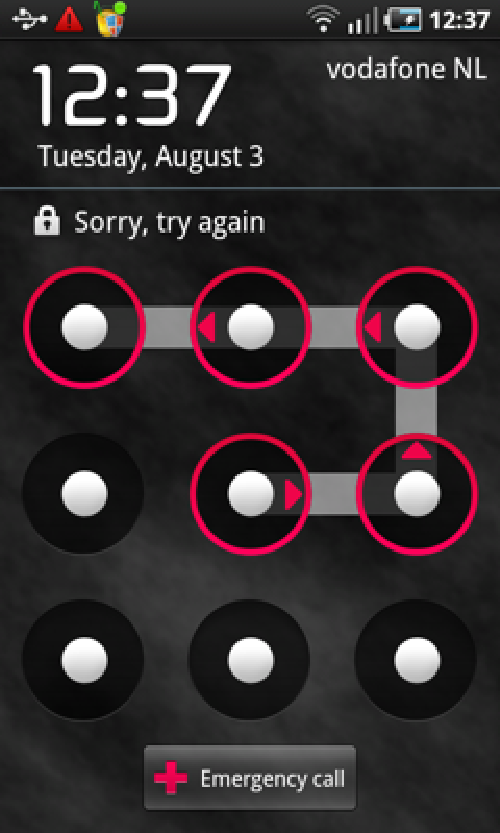
\includegraphics{./phonelock.pdf}
}
\end{center}

Here we will explore how many unique patterns are available
when drawing such patterns to connect ``dots'', such as shown in the
figure.
We assume that people put their finger on one ``dot'' and then only ever move
one position left, right, up or down (but never diagonally) at
a time. You are not allowed to return to a ``dot'' once it has
been visited once. If we number the first position in our path as $1$, the
second as $2$ and so on, then beginning in the top left-hand
corner, some of the possible patterns of 9 moves are~:
\begin{verbatim}

1 2 3      1 2 3      1 2 3
6 5 4      8 9 4      8 7 4
7 8 9      7 6 5      9 6 5

\end{verbatim}

\begin{exercise}
Write a program that computes and outputs all the valid paths.
Use \textbf{recursion} to achieve this.
\begin{itemize}
\item How many different patterns of length $9$ are
    available on a $3 \times 3$ grid, if the user begins in
    the top left corner ?

\item How many different patterns of length $9$ are
    available on a $3 \times 3$ grid, if the user begins in
    the middle left ?

\item How many different patterns of length $7$ are
    available on a $3 \times 3$ grid, if the user begins in
    the top left corner ?

\item How many different patterns of length $25$ are
    available on a $5 \times 5$ grid, if the user begins in
    the top left corner ?
\end{itemize}
\end{exercise}


\nsection{SDL - Intro}

Many programming languages have no inherent graphics capabilities.
To get windows to appear on the screen, or to draw lines and shapes,
you need to make use of an external library. Here we use SDL\footnote{
actually, we are using the most recent version SDL2, which is installed
on all the lab machines}, a cross-platform library providing the user with
(amongst other things) such graphical capabilities.

\wwwurl{https://www.libsdl.org/}

The use of SDL is, unsurprisingly, non-trival, so some simple wrapper
files have been created (\verb^neillsdl2.c^ and \verb^neillsdl2.h^).
These give you some simple functions to initialise a window, draw
rectangles, wait for the user to press a key etc.

An example program using this functionality is
provided in a file \verb^demo_neillsdl2.c^.

This program initialises a window, then sits in a loop, drawing
randomly positioned and coloured squares, until the
user presses the mouse or a key. 

\begin{exercise}
Using the \verb^Makefile^ provided, compile and run this program.

SDL is already installed on lab machines. At home, if you're using a
ubuntu-style linux machine, use: \verb^sudo apt install libsdl2-dev^
to install it.
\end{exercise}


\nsection{Word Ladders}

In this game, made famous by the author Lewis Caroll, and investigated by many Computer Scientists including Donald Knuth,
you find missing words to complete a sequence.
For instance, you might be asked how go from ``WILD'' to ``TAME''
by only changing one character at a time:
\begin{center}
\begin{tikzpicture}
\matrix (wild2tame) [matrix of nodes]
{
W&I&L&D \\
W&I&L&E \\
T&I&L&E \\
T&A&L&E \\
T&A&M&E \\
};
\end{tikzpicture}
\end{center}


\tikzset{word ladder/.style={
  matrix of nodes
  , execute at empty cell={\node[draw=gray,text=gray,fill=white]{0};}
  , nodes in empty cells=false
  , nodes={shape=rectangle, draw=none,fill=none,text=black,minimum width=0.6cm,minimum height=0.35cm,outer sep=0pt,align=center,inner sep=0pt,font=\small}
  , row sep={0.35cm,between origins}
  , column sep={0.6cm,between origins}
},
}

\tikzset{spacehash board/.style={
  matrix of nodes
  , execute at empty cell={\node[draw=gray,text=gray,fill=white]{ };}
  , nodes in empty cells=false
  , nodes={draw=gray,fill=ocre,text=gray,text depth=0.5ex,text height=2ex,text width=1em,outer sep=0pt,align=center,inner sep=0pt}
  , row sep={#1,between origins}
  , column sep={#1,between origins}
},
}

\tikzset{noughtsone board/.style={
  matrix of nodes
  , execute at empty cell={\node[draw=gray,text=gray,fill=white]{0};}
  , nodes in empty cells=false
  , nodes={draw=gray,fill=ocre,text=gray,minimum width=#1,minimum height=#1,outer sep=0pt,align=center,inner sep=0pt}
  , row sep={#1,between origins}
  , column sep={#1,between origins}
},
  noughtsone board/.default=0.5cm
}

\tikzset{twocolour board/.style={
  matrix of nodes
  , execute at empty cell={\node[text=white,fill=white]{+};}
  , nodes in empty cells=false
  , nodes={draw=gray,fill=ocre,minimum width=#1,minimum height=#1,outer sep=0pt,align=center,inner sep=0pt,font=\tiny}
  , text=ocre
  , row sep={#1,between origins}
  , column sep={#1,between origins}
},
  twocolour board/.default=0.5cm
}
\tikzset{twocolour board/.style={
  matrix of nodes
  , execute at empty cell={\node[text=white,fill=white]{+};}
  , nodes in empty cells=false
  , nodes={draw=gray,fill=ocre,minimum width=#1,minimum height=#1,outer sep=0pt,align=center,inner sep=0pt,font=\tiny}
  , text=ocre
  , row sep={#1,between origins}
  , column sep={#1,between origins}
},
  twocolour board/.default=0.5cm
}

%% Candy Crush-style games, colour & label
\tikzset{crushstyle board/.style={
  matrix of nodes
  , nodes={draw=gray,fill=ocre,minimum width=#1,minimum height=#1,outer sep=0pt,align=center,inner sep=0pt,font=\tiny}
  , text=ocre
  , row sep={#1,between origins}
  , column sep={#1,between origins}
},
  crushstyle board/.default=0.5cm
}

%% WaTor-style games, colour & label
\tikzset{watorstyle board/.style={
  matrix of nodes
  , nodes={fill=cyan,minimum width=#1,minimum height=#1,outer sep=0pt,align=center,inner sep=0pt,font=\tiny}
  , text=black
  , row sep={#1,between origins}
  , column sep={#1,between origins}
},
  watorstyle board/.default=0.25cm
}

%% 8-tile style
\tikzset{eighttilestyle board/.style={
  matrix of nodes, ampersand replacement={\&}
  , execute at empty cell={\node[draw=gray,text=gray,fill=gray]{0};}
  , nodes={fill=gray,minimum width=#1,minimum height=#1,outer sep=0pt,align=center,inner sep=0pt,font=\tiny}
  , text=ocre
  , row sep={#1,between origins}
  , column sep={#1,between origins}
},
  eighttilestyle board/.default=0.25cm
}

\tikzset{sixelstyle/.style={
  matrix of nodes, ampersand replacement={\&}
  , nodes={draw=black,fill=gray,text=gray
     %,minimum height=1pt, minimum width=1pt
     %,row sep=1pt, column sep=1pt
}
},
   sixelstyle/.default=0.3em
}

\tikzset{sepsixstyle/.style={
  matrix of nodes, ampersand replacement={\&}
  , nodes={draw=white,fill=gray,text=gray,
     minimum height=1pt, minimum width=1pt,
     row sep=1pt, column sep=1pt}
},
   sixelstyle/.default=0.3em
}


In a heavily constrained version of this game we make some simplifying assumptions:
\begin{itemize}
\item Words are always four letters long.
\item We only seek ladders of five words in total. 
\item Only one letter is changed at a time.
\item A letter is only changed from its initial state, to its target state. This is important, since if you decide to change the second letter then you will always know what it's changing from, to what it's changing to.
\end{itemize}

So, in the example above, it is enough to give the first word, the last word, and the position of the character which changed on each line. On line one, the fourth letter `D' was changed to an `E', on the next line the first character `W' was changed to a `T' and so on. The whole ladder can be defined by ``WILD'', ``TAME'' and the sequence $4,1,2,3$. 

\begin{center}
\begin{tikzpicture}
\matrix (wild2tame) [matrix of nodes]
{
W&I&L&D \\
W&I&L&E \\
T&I&L&E \\
T&A&L&E \\
T&A&M&E \\
};
\node at (wild2tame-1-4) [minimum width=14pt,shape=circle,draw=red,fill=ocre,fill opacity=0.4]{};
\node at (wild2tame-2-1) [minimum width=14pt,shape=circle,draw=red,fill=ocre,fill opacity=0.4]{};
\node at (wild2tame-3-2) [minimum width=14pt,shape=circle,draw=red,fill=ocre,fill opacity=0.4]{};
\node at (wild2tame-4-3) [minimum width=14pt,shape=circle,draw=red,fill=ocre,fill opacity=0.4]{};
\end{tikzpicture}
\end{center}

Since each letter changes exactly once, the order in which this happens is a {\em permutation} of the numbers $1,2,3,4$, which we have looked at elsewhere.
 
\begin{exercise}
For the constrained version of the game, given a file of valid four
letter words, write a program which when given two words on the command
line (\verb^argv[1]^ and \verb^argv[2]^) outputs the correct solution,
if available. Use an exhaustive search over the $24$ permutations until
one leads to no invalid words being required.
Make sure your program works, with amongst others, the following:
\begin{center}
\begin{tikzpicture}
\matrix (wild2tame) [matrix of nodes]
{
C&O&L&D \\
C&O&R&D \\
C&A&R&D \\
W&A&R&D \\
W&A&R&M \\
};
\node at (wild2tame-1-3) [minimum width=14pt,shape=circle,draw=red,fill=ocre,fill opacity=0.4]{};
\node at (wild2tame-2-2) [minimum width=14pt,shape=circle,draw=red,fill=ocre,fill opacity=0.4]{};
\node at (wild2tame-3-1) [minimum width=14pt,shape=circle,draw=red,fill=ocre,fill opacity=0.4]{};
\node at (wild2tame-4-4) [minimum width=14pt,shape=circle,draw=red,fill=ocre,fill opacity=0.4]{};
\end{tikzpicture}
\hspace*{1in}
\begin{tikzpicture}
\matrix (wild2tame) [matrix of nodes]
{
P&O&K&E \\
P&O&L&E \\
P&O&L&L \\
M&O&L&L \\
M&A&L&L \\
};
\node at (wild2tame-1-3) [minimum width=14pt,shape=circle,draw=red,fill=ocre,fill opacity=0.4]{};
\node at (wild2tame-2-4) [minimum width=14pt,shape=circle,draw=red,fill=ocre,fill opacity=0.4]{};
\node at (wild2tame-3-1) [minimum width=14pt,shape=circle,draw=red,fill=ocre,fill opacity=0.4]{};
\node at (wild2tame-4-2) [minimum width=14pt,shape=circle,draw=red,fill=ocre,fill opacity=0.4]{};
\end{tikzpicture}
\hspace*{1in}
\begin{tikzpicture}
\matrix (wild2tame) [matrix of nodes]
{
C&U&B&E \\
C&U&B&S \\
T&U&B&S \\
T&U&N&S \\
T&O&N&S \\
};
\node at (wild2tame-1-4) [minimum width=14pt,shape=circle,draw=red,fill=ocre,fill opacity=0.4]{};
\node at (wild2tame-2-1) [minimum width=14pt,shape=circle,draw=red,fill=ocre,fill opacity=0.4]{};
\node at (wild2tame-3-3) [minimum width=14pt,shape=circle,draw=red,fill=ocre,fill opacity=0.4]{};
\node at (wild2tame-4-2) [minimum width=14pt,shape=circle,draw=red,fill=ocre,fill opacity=0.4]{};
\end{tikzpicture}
\end{center}
\end{exercise}

\begin{exercise}
Adapt the program above so that if the first and last words share a letter (the edit distance is less than $4$), you can find the word ladder required, as in:
\begin{center}
\begin{tikzpicture}
\matrix (wild2tame) [matrix of nodes]
{
W&A&S&P \\
W&A&S&H \\
W&I&S&H \\
F&I&S&H \\
};
\node at (wild2tame-1-4) [minimum width=14pt,shape=circle,draw=red,fill=ocre,fill opacity=0.4]{};
\node at (wild2tame-2-2) [minimum width=14pt,shape=circle,draw=red,fill=ocre,fill opacity=0.4]{};
\node at (wild2tame-3-1) [minimum width=14pt,shape=circle,draw=red,fill=ocre,fill opacity=0.4]{};
\end{tikzpicture}
\end{center}
\end{exercise}

\tikzset{word ladder/.style={
  matrix of nodes
  , execute at empty cell={\node[draw=gray,text=gray,fill=white]{0};}
  , nodes in empty cells=false
  , nodes={shape=rectangle, draw=none,fill=none,text=black,minimum width=0.6cm,minimum height=0.35cm,outer sep=0pt,align=center,inner sep=0pt,font=\small}
  , row sep={0.35cm,between origins}
  , column sep={0.6cm,between origins}
},
}

\tikzset{spacehash board/.style={
  matrix of nodes
  , execute at empty cell={\node[draw=gray,text=gray,fill=white]{ };}
  , nodes in empty cells=false
  , nodes={draw=gray,fill=ocre,text=gray,text depth=0.5ex,text height=2ex,text width=1em,outer sep=0pt,align=center,inner sep=0pt}
  , row sep={#1,between origins}
  , column sep={#1,between origins}
},
}

\tikzset{noughtsone board/.style={
  matrix of nodes
  , execute at empty cell={\node[draw=gray,text=gray,fill=white]{0};}
  , nodes in empty cells=false
  , nodes={draw=gray,fill=ocre,text=gray,minimum width=#1,minimum height=#1,outer sep=0pt,align=center,inner sep=0pt}
  , row sep={#1,between origins}
  , column sep={#1,between origins}
},
  noughtsone board/.default=0.5cm
}

\tikzset{twocolour board/.style={
  matrix of nodes
  , execute at empty cell={\node[text=white,fill=white]{+};}
  , nodes in empty cells=false
  , nodes={draw=gray,fill=ocre,minimum width=#1,minimum height=#1,outer sep=0pt,align=center,inner sep=0pt,font=\tiny}
  , text=ocre
  , row sep={#1,between origins}
  , column sep={#1,between origins}
},
  twocolour board/.default=0.5cm
}
\tikzset{twocolour board/.style={
  matrix of nodes
  , execute at empty cell={\node[text=white,fill=white]{+};}
  , nodes in empty cells=false
  , nodes={draw=gray,fill=ocre,minimum width=#1,minimum height=#1,outer sep=0pt,align=center,inner sep=0pt,font=\tiny}
  , text=ocre
  , row sep={#1,between origins}
  , column sep={#1,between origins}
},
  twocolour board/.default=0.5cm
}

%% Candy Crush-style games, colour & label
\tikzset{crushstyle board/.style={
  matrix of nodes
  , nodes={draw=gray,fill=ocre,minimum width=#1,minimum height=#1,outer sep=0pt,align=center,inner sep=0pt,font=\tiny}
  , text=ocre
  , row sep={#1,between origins}
  , column sep={#1,between origins}
},
  crushstyle board/.default=0.5cm
}

%% WaTor-style games, colour & label
\tikzset{watorstyle board/.style={
  matrix of nodes
  , nodes={fill=cyan,minimum width=#1,minimum height=#1,outer sep=0pt,align=center,inner sep=0pt,font=\tiny}
  , text=black
  , row sep={#1,between origins}
  , column sep={#1,between origins}
},
  watorstyle board/.default=0.25cm
}

%% 8-tile style
\tikzset{eighttilestyle board/.style={
  matrix of nodes, ampersand replacement={\&}
  , execute at empty cell={\node[draw=gray,text=gray,fill=gray]{0};}
  , nodes={fill=gray,minimum width=#1,minimum height=#1,outer sep=0pt,align=center,inner sep=0pt,font=\tiny}
  , text=ocre
  , row sep={#1,between origins}
  , column sep={#1,between origins}
},
  eighttilestyle board/.default=0.25cm
}

\tikzset{sixelstyle/.style={
  matrix of nodes, ampersand replacement={\&}
  , nodes={draw=black,fill=gray,text=gray
     %,minimum height=1pt, minimum width=1pt
     %,row sep=1pt, column sep=1pt
}
},
   sixelstyle/.default=0.3em
}

\tikzset{sepsixstyle/.style={
  matrix of nodes, ampersand replacement={\&}
  , nodes={draw=white,fill=gray,text=gray,
     minimum height=1pt, minimum width=1pt,
     row sep=1pt, column sep=1pt}
},
   sixelstyle/.default=0.3em
}


For the ``full'' version of Wordladder, you make no assumptions
about the number of words that are needed to make the ladder, although
we do assume that all the words in the ladder are the same size.

\begin{exercise}
To achieve this, you could make a
list of all the words, and for all words an \verb^edit distance^ of $1$ away from
the initial word, mark these and store their `parent'. Now, go through
this list, and for all words marked, find words which are distance $1$
from these, and hence distance $2$ from the initial word. Mark these and
retain their parent. Be careful you don't use words
already marked. If the word ladder is possible, you'll eventually find the
solution, and via the record of the parents, have the correct route.
This is shown for the word ladder CAT to DOG in Figure~\ref{wordladder:fig_catdog}
using a very small subset of the possible three letter words.
\end{exercise}

\begin{figure}
\begin{center}
\begin{tikzpicture}
\matrix (catdog) [word ladder]
{
\node (but) {but}; \\
\node (cat) {cat}; \\
\node (cob) {cob}; \\
\node (cod) {cod}; \\
\node (cog) {cog}; \\
\node (con) {con}; \\
\node (con) {con}; \\
\node (cot) {cot}; \\
\node (cow) {cow}; \\
\node (cub) {cub}; \\
\node (cud) {cud}; \\
\node (cue) {cue}; \\
\node (cup) {cup}; \\
\node (cur) {cur}; \\
\node (cut) {cut}; \\
\node (dog) {dog}; \\
\node (dot) {dot}; \\
\node (got) {got}; \\
\node (gut) {gut}; \\
\node (hut) {hut}; \\
\node (jot) {jot}; \\
\node (lot) {lot}; \\
\node (not) {not}; \\
\node (nut) {nut}; \\
\node (pot) {pot}; \\
\node (put) {put}; \\
\node (rot) {rot}; \\
\node (rut) {rut}; \\
\node (tot) {tot}; \\
};
\draw [->,ocre] (cot.west) to [in=0,out=0,bend left=90] (cat.west); 
\draw [->,ocre] (cut.east) to [in=0,out=0,bend right=90] (cat.east); 
\end{tikzpicture}
\begin{tikzpicture}
\matrix (catdog) [word ladder]
{
\node (but) {but}; \\
\node (cat) {cat}; \\
\node (cob) {cob}; \\
\node (cod) {cod}; \\
\node (cog) {cog}; \\
\node (con) {con}; \\
\node (con) {con}; \\
\node (cot) {cot}; \\
\node (cow) {cow}; \\
\node (cub) {cub}; \\
\node (cud) {cud}; \\
\node (cue) {cue}; \\
\node (cup) {cup}; \\
\node (cur) {cur}; \\
\node (cut) {cut}; \\
\node (dog) {dog}; \\
\node (dot) {dot}; \\
\node (got) {got}; \\
\node (gut) {gut}; \\
\node (hut) {hut}; \\
\node (jot) {jot}; \\
\node (lot) {lot}; \\
\node (not) {not}; \\
\node (nut) {nut}; \\
\node (pot) {pot}; \\
\node (put) {put}; \\
\node (rot) {rot}; \\
\node (rut) {rut}; \\
\node (tot) {tot}; \\
};
\draw [->,lightgray,opacity=0.5] (cot.west) to [in=0,out=0,bend left=90] (cat.west); 
\draw [->,lightgray,opacity=0.5] (cut.east) to [in=0,out=0,bend right=90] (cat.east); 

\draw [->,ocre] (but.east) to [in=0,out=0,bend left=90] (cut.east); 
\draw [->,ocre] (nut.east) to [in=0,out=0,bend right=90] (cut.east); 
\draw [->,ocre] (gut.east) to [in=0,out=0,bend right=90] (cut.east); 
\draw [->,ocre] (hut.east) to [in=0,out=0,bend right=90] (cut.east); 
\draw [->,ocre] (put.east) to [in=0,out=0,bend right=90] (cut.east); 
\draw [->,ocre] (cub.east) to [in=0,out=0,bend left=90] (cut.east); 
\draw [->,ocre] (rut.east) to [in=0,out=0,bend right=90] (cut.east); 
\draw [->,ocre] (cud.east) to [in=0,out=0,bend left=90] (cut.east); 
\draw [->,ocre] (cue.east) to [in=0,out=0,bend left=90] (cut.east); 
\draw [->,ocre] (cup.east) to [in=0,out=0,bend left=90] (cut.east); 
\draw [->,ocre] (cur.east) to [in=0,out=0,bend left=90] (cut.east); 

\draw [->,ocre] (cog.west) to [in=0,out=0,bend right=90] (cot.west);
\draw [->,ocre] (cod.west) to [in=0,out=0,bend right=90] (cot.west);
\draw [->,ocre] (cob.west) to [in=0,out=0,bend right=90] (cot.west);
\draw [->,ocre] (con.west) to [in=0,out=0,bend right=90] (cot.west);

\draw [->,ocre] (cow.west) to [in=0,out=0,bend left=90] (cot.west);
\draw [->,ocre] (dot.west) to [in=0,out=0,bend left=90] (cot.west);
\draw [->,ocre] (got.west) to [in=0,out=0,bend left=90] (cot.west);
\draw [->,ocre] (jot.west) to [in=0,out=0,bend left=90] (cot.west);
\draw [->,ocre] (lot.west) to [in=0,out=0,bend left=90] (cot.west);
\draw [->,ocre] (not.west) to [in=0,out=0,bend left=90] (cot.west);
\draw [->,ocre] (pot.west) to [in=0,out=0,bend left=90] (cot.west);
\draw [->,ocre] (rot.west) to [in=0,out=0,bend left=90] (cot.west);
\draw [->,ocre] (tot.west) to [in=0,out=0,bend left=90] (cot.west);
\end{tikzpicture}
\begin{tikzpicture}
\matrix (catdog) [word ladder]
{
\node (but) {but}; \\
\node (cat) {cat}; \\
\node (cob) {cob}; \\
\node (cod) {cod}; \\
\node (cog) {cog}; \\
\node (con) {con}; \\
\node (con) {con}; \\
\node (cot) {cot}; \\
\node (cow) {cow}; \\
\node (cub) {cub}; \\
\node (cud) {cud}; \\
\node (cue) {cue}; \\
\node (cup) {cup}; \\
\node (cur) {cur}; \\
\node (cut) {cut}; \\
\node (dog) {dog}; \\
\node (dot) {dot}; \\
\node (got) {got}; \\
\node (gut) {gut}; \\
\node (hut) {hut}; \\
\node (jot) {jot}; \\
\node (lot) {lot}; \\
\node (not) {not}; \\
\node (nut) {nut}; \\
\node (pot) {pot}; \\
\node (put) {put}; \\
\node (rot) {rot}; \\
\node (rut) {rut}; \\
\node (tot) {tot}; \\
};
\draw [->,lightgray,opacity=0.5] (cot.west) to [in=0,out=0,bend left=90] (cat.west); 
\draw [->,lightgray,opacity=0.5] (cut.east) to [in=0,out=0,bend right=90] (cat.east); 

\draw [->,lightgray,opacity=0.5] (but.east) to [in=0,out=0,bend left=90] (cut.east); 
\draw [->,lightgray,opacity=0.5] (nut.east) to [in=0,out=0,bend right=90] (cut.east); 
\draw [->,lightgray,opacity=0.5] (gut.east) to [in=0,out=0,bend right=90] (cut.east); 
\draw [->,lightgray,opacity=0.5] (hut.east) to [in=0,out=0,bend right=90] (cut.east); 
\draw [->,lightgray,opacity=0.5] (put.east) to [in=0,out=0,bend right=90] (cut.east); 
\draw [->,lightgray,opacity=0.5] (cub.east) to [in=0,out=0,bend left=90] (cut.east); 
\draw [->,lightgray,opacity=0.5] (rut.east) to [in=0,out=0,bend right=90] (cut.east); 
\draw [->,lightgray,opacity=0.5] (cud.east) to [in=0,out=0,bend left=90] (cut.east); 
\draw [->,lightgray,opacity=0.5] (cue.east) to [in=0,out=0,bend left=90] (cut.east); 
\draw [->,lightgray,opacity=0.5] (cup.east) to [in=0,out=0,bend left=90] (cut.east); 
\draw [->,lightgray,opacity=0.5] (cur.east) to [in=0,out=0,bend left=90] (cut.east); 

\draw [->,lightgray,opacity=0.5] (cog.west) to [in=0,out=0,bend right=90] (cot.west);
\draw [->,lightgray,opacity=0.5] (cod.west) to [in=0,out=0,bend right=90] (cot.west);
\draw [->,lightgray,opacity=0.5] (cob.west) to [in=0,out=0,bend right=90] (cot.west);
\draw [->,lightgray,opacity=0.5] (con.west) to [in=0,out=0,bend right=90] (cot.west);

\draw [->,lightgray,opacity=0.5] (cow.west) to [in=0,out=0,bend left=90] (cot.west);
\draw [->,lightgray,opacity=0.5] (dot.west) to [in=0,out=0,bend left=90] (cot.west);
\draw [->,lightgray,opacity=0.5] (got.west) to [in=0,out=0,bend left=90] (cot.west);
\draw [->,lightgray,opacity=0.5] (jot.west) to [in=0,out=0,bend left=90] (cot.west);
\draw [->,lightgray,opacity=0.5] (lot.west) to [in=0,out=0,bend left=90] (cot.west);
\draw [->,lightgray,opacity=0.5] (not.west) to [in=0,out=0,bend left=90] (cot.west);
\draw [->,lightgray,opacity=0.5] (pot.west) to [in=0,out=0,bend left=90] (cot.west);
\draw [->,lightgray,opacity=0.5] (rot.west) to [in=0,out=0,bend left=90] (cot.west);
\draw [->,lightgray,opacity=0.5] (tot.west) to [in=0,out=0,bend left=90] (cot.west);

\draw [->,ocre,thick] (dog.west) to [in=0,out=0,bend right=60] (dot.west);
\end{tikzpicture}
\end{center}
\caption{Word Ladder from CAT to DOG. (Left) Words which are distance one from CAT are COT and CUT. (Middle) Words which are distance one from CUT and COT, which includes amongst others, DOT. (Right) DOG is distance one from DOT. We now have our route, via the pointers, back to CAT.}
\label{wordladder:fig_catdog}
\end{figure}


\nsection{The Devil's Dartboard}

\tikzstyle{wired}=[draw=gray!30, line width=0.15mm]
\tikzstyle{number}=[anchor=center, color=white]
% Sectors are numbered 0-19 counterclockwise from the top.

% \strip{color}{sector}{outer_radius}{inner_radius}
\newcommand{\strip}[4]{
    \filldraw[#1, wired]
      ({18 *  #2}      :                   #3) arc
      ({18 *  #2}      : {18 * (#2 + 1)} : #3) --
      ({18 * (#2 + 1)} :                   #4) arc
      ({18 * (#2 + 1)} : {18 *  #2}      : #4) -- cycle;
}

% \sector{color}{sector}{radius}
\newcommand{\sector}[3]{
    \filldraw[#1, wired]
      (0, 0) --
      ({18 * #2} :                   #3) arc
      ({18 * #2} : {18 * (#2 + 1)} : #3) -- cycle;
}

\newcommand{\dartboard}{
 % These are the official dartboard dimensions as per BDO's regulations.
  % The whole board's background.
  \fill[black] (0, 0) circle (225.5mm);
  % Even sections.
  \foreach\i in {0,2,...,18} {
    \sector{black}{\i}{162mm}
    \strip{red}{\i}{170mm}{162mm} % Double strip.
    \strip{red}{\i}{107mm}{ 99mm} % Treble strip.
  }
  % Odd sections.
  \foreach\i in {1,3,...,19} {
    \sector{white}{\i}{162mm}
    \strip{green}{\i}{170mm}{162mm} % Double strip.
    \strip{green}{\i}{107mm}{ 99mm} % Treble strip.
  }
  % Bull's ring and eye.
  \filldraw[green, wired] (0, 0) circle (15.9mm);
  \filldraw[red,   wired] (0, 0) circle (6.35mm);
 % Labels.
  \foreach \sector/\label in {%
      0/20,  1/ 1,  2/18,  3/ 4,  4/13,
      5/ 6,  6/10,  7/15,  8/ 2,  9/17,
     10/ 3, 11/19, 12/ 7, 13/16, 14/ 8,
     15/11, 16/14, 17/ 9, 18/12, 19/ 5}%
  {
    \node[number] at ({18 * (-\sector + .5)} : 197.75mm) {\sffamily\label};
  }
}


\begin{figure}[h]
\centering
\begin{tikzpicture}[scale=.10]
\begin{scope}[rotate=81]
\dartboard
\end{scope}
\begin{scope}
\node[text=black] (trb) at (-200mm, 300mm) {Treble 20};
\draw [-Circle,ocre] (trb.east) -- (-0mm,100mm);
\node[text=black] (dbl) at (175mm, 300mm) {Double 4};
\draw [-Circle,ocre] (dbl.south) -- (135mm,95mm);
\end{scope}
\end{tikzpicture}
\end{figure}

In the traditional `pub' game, darts, there are 62 different possible scores~:
single 1 - 20 (the white and black areas), double 1 - 20 (the outer red and green segments)
(i.e. 2, 4, 6, 8 $\ldots$), treble 1 - 20 (i.e. 3, 6, 9, 12 $\ldots$) (the inner red or green segments), 25 (small green circle) and 50 (the small red inner circle).


It's not obvious, if you were inventing darts from scratch, how best to
lay out the numbers. The London board shown seems to have small numbers near high numbers,
so that if you just miss the $20$ for example, you'll hit a small number instead.

Here we look at a measure for the `difficulty' of a dartboard.
One approach is to simply sum up the values of adjacent triples, squaring 
this number. So for the London board shown, this would be:
\begin{math}
(20+1+18)^2 + (1+18+4)^2 + (18+4+13)^2 \dots (5+20+1)^2 = 20478
\end{math}

For our purposes a {\bf lower} number is better\footnote{It's beyond
the scope here to explain why!}. For more details see~:
\wwwurl{http://www.mathpages.com/home/kmath025.htm}

\begin{exercise}
Write a program that repeatedly chooses two
positions on the board at random and swaps them. If this leads to a lower cost,
keep the board. If not, unswap them. Repeat this {\it greedy search}
$5000000$ times, and print out the best board found.
Begin with the trivial monotonic sequence.
The output may look something like~:
\begin{terminaloutput}
Total = 19966 :  3 19 11  2 18 12  1 20 10  4 16  8
14  5 13 15  6  7 17  9 
\end{terminaloutput}
or
\begin{terminaloutput}
Total = 19910 :  3 18 10  5 16  9  8 14 11  4 19  6
7 20  2 13 15  1 17 12 
\end{terminaloutput}

Is the score of $19874$ the lowest possible that may be obtained via this technique~?
\end{exercise}

%\begin{exercise}
%You can also argue that the $16$ next to the $8$ is a bad idea. Alternate
%odd-and-even numbers is appealing.
%Is~:
%\begin{terminaloutput}
%Total = 19886 : 20  3 10 19  2 11 18  1 14 13  4 15 12  5 16  9  6 17  8  7 
%\end{terminaloutput}
%the best possible ?
%\end{exercise}
%
%
%\wwwurl{https://cms.math.ca/crux/v26/n4/page215-217.pdf}
%
%Here is a polynomial-time algorithm that, if it does not always produce a
%Devil's Dartboard, seems to come pretty close, especially for large $n$.
%The permutation p is defined by induction. Choose p(k + 1) such that the
%3-sum $p(k-1) + p(k) + p(k + 1)$ is as close as possible to the mean $m =
%3(n + 1)/2$ of the 3-sums. In the case of a tie, select $p(k + 1)$ so that
%consecutive 3-sums (different from $m$) fall on opposite sides of $m$,
%beginning with a 3-sum greater than $m$. To get the induction started,
%set $p(1) = n$ and $p(2) = 1$.
%
%For example, if $n = 6$, we have $m = 3(6+ 1)/2 = 10.5$. The algorithm
%then produces the Devil's Dartboard 6, 1, 4, 5, 2, 3.
%
%For $n = 20$, the algorithm generates the permutation $20, 1, 11, 19,
%2, 10, 18, 4, 9, 17, 6, 8, 16, 7, 12, 13, 5, 14, 15, 3$ which is not as
%good as the traditional London board.






\nsection{Maze}

Escaping from a maze can be done in several ways (ink-blotting, righthand-on-wall etc.)
but here we look at recursion.

\begin{exercise}
Write a program to read in a maze typed by a user via the filename passed to \verb^argv[1]^.
You can assume the maze will be no larger than $20 \times 20$,
walls are designated by with a \verb^#^ and the rest are
spaces. The entrance can be assumed to be the gap in the wall closest to
(but not necessarilty exactly at) the top lefthand corner.
The sizes of the maze are given on the first line of the file (width,height).
Write a program that finds the route through a maze, read from this file,
and prints out the solution (if one exists) using full stops.
If the program succeeds it should exit with a status of \verb^0^,
or if no route exists it should exit with a status of \verb^1^.
\end{exercise}

\newcommand{\W}{|[fill=ocre,text=white]|\#}
\newcommand{\R}{|[fill=white,text=gray]|.}

\begin{tikzpicture}[every node/.style={anchor=base,text depth=.5ex,text height=2ex,text width=1em,outer sep=0pt,align=center,inner sep=0pt}]
\matrix [matrix of nodes,draw=white,nodes in empty cells]
{
\W&\W&\W&\W&\W&\W&\W&\W&\W&\W\\
\R&\R&\W&\R&\R&\R&\R&\R&\R&\W\\
\W&\R&\W&\R&\W&\R&\W&\W&\R&\W\\
\W&\R&\W&\R&\W&\W&\W&\W&\R&\W\\
\W&\R&\W&\R&\R&\R&\R&\W&\R&\W\\
\W&\R&\W&\R&\W&\W&\W&\W&\R&\W\\
\W&\R&\W&\R&\R&\R&\R&\W&\R&\W\\
\W&\R&\W&\W&\W&\W&\R&\W&\R&\W\\
\W&\R&\R&\R&\R&\R&\R&\W&\R&\R\\
\W&\W&\W&\W&\W&\W&\W&\W&\W&\W\\
};
\end{tikzpicture}


\chapterimage{../Pictures/Insertionsort-edited.png}
\chapter{Lists, Insertion Sort \& more Recursion}

\nsection{A Simple Spelling Checker}

Here, we reads words one at a time
from file and carefully place them in the {\bf correct} part of
our data structure. This has a complexty of $O(n^2)$.

For this purpose, a list of valid words (unsorted) is available
from the usual place.

\begin{exercise}
\label{ex:arrayinsertsort}
Write a program which, based on a
list implemented using {\bf arrays}, reads the words in
one at a time, inserting them into the {\bf correct} part of the list
so that the words are alphabetically sorted.
The name of the file should be passed as \verb^argv[1]^,
and you can assume the array is of a fixed-size,
and large enough to hold all words.
How long does it take to build the list~?
\end{exercise}

\begin{exercise}
Now extend Exercise~\ref{ex:arrayinsertsort}
so that when the user is prompted for a word,
they are told whether this word is present in the list or not.
Use a binary search to achieve this.
How much faster is this than a linear search~?
\end{exercise}

\begin{exercise}
Write a program which, based on a
linked list data structure, reads the words in
one at a time, inserting them into the {\bf correct} part of the list
so that the words are alphabetically sorted.
The name of the file should be passed as \verb^argv[1]^.
How long does it take to build the list~?
\end{exercise}



\nsection{Prime Factors}

\wwwurl{en.wikipedia.org/wiki/Prime_factor}

It is well known that any positive integer has a single {\it unique}
prime factorization, e.g.:

$210 = 7 \times 5 \times 3 \times 2$ (the numbers $7,5,3$ and
$2$ are all prime).

$117 = 13 \times 3 \times 3$ (the numbers $13$ and $3$ are all
prime).

$197$ is prime, so has only itself (and $1$, which we ignore)
as a factor.

\begin{exercise}
Write a program that, for any given positive integer input
using \verb^argv[1]^, lists the prime factors, e.g.:

\begin{terminaloutput}
[campbell@icy]% ./primefacts 210
7 5 3 2

[campbell@icy]% ./primefacts 117
13 3 3
\end{terminaloutput}
\end{exercise}

\begin{exercise}
To make the output of the above program briefer,
many prefer to show the factors
expressed by their power, as in~:
\[
768 = 2 \times 2 \times 2 \times 2 \times 2 \times 2 \times 2 \times 3
\]
could be better expressed as~:
\[
768 = 2^8 \times 3
\]
Write a program to show the factorisation of a number
in this more compact style~:
\begin{terminaloutput}
 % ./primefactors 27000
27000 = 1 x 2^3 x 3^3 x 5^3
 % ./primefactors 31          
31 = 1 x 31
 % ./primefactors 38654705664
38654705664 = 1 x 2^32 x 3^2
\end{terminaloutput}
\end{exercise}

\toohard

\begin{exercise}
For a beautiful visualisation of prime factors, see:\\
\wwwurl{www.datapointed.net/visualizations/math/factorization/animated-diagrams}
Adapt the program above to output a
pattern similar to the animated display above, using SDL, but
only for a single number, not an animation.
\begin{center}
\scalebox{0.3}{

\includegraphics{./primevis.pdf}
}
\end{center}
\end{exercise}


\nsection{Sierpinski Carpet}

\wwwurl{en.wikipedia.org/wiki/Sierpinski_carpet}

The square is cut into 9 congruent subsquares in a 3-by-3 grid, and
the central subsquare is removed. The same procedure is then applied
recursively to the remaining 8 subsquares, ad infinitum.


\wwwurl{http://www.evilmadscientist.com/2008/sierpinski-cookies/}

\begin{exercise}
Write a program that, in plain text, produces a Sierpinski Carpet.
\end{exercise}

\begin{exercise}
Write a program that, using \verb^neillsimplescreen^,
produces a Sierpinski Carpet.
\end{exercise}

\begin{exercise}
Write a program that, using SDL, produces a Sierpinski Carpet.
\end{exercise}


\nsection{Sierpinski Squares}

See also~:
\wwwurl{en.wikipedia.org/wiki/Sierpinski_triangle}

The Sierpinski triangle has the overall shape of an equilateral 
triangle, recursively subdivded into four smaller triangles~:
\begin{center}
\centering
\includegraphics[scale=0.30]{./sierpinsky_curve.pdf}
\end{center}

However, we can approximate it by recursively drawing a square
as three smaller squares, as show below~:
\begin{center}
\centering
\includegraphics{./sierpinsky_squares.pdf}
\end{center}

The recursion should terminate when the squares are too small to draw with any more detail (e.g. one pixel, or one character in size).

\begin{exercise}
Write a program that, in plain text, produces a Sierpinski Triangle.
\end{exercise}

\begin{exercise}
Write a program that, using \verb^neillsimplescreen^,
produces a Sierpinski Triangle.
\end{exercise}

\begin{exercise}
Write a program that, using SDL, produces a Sierpinski Triangle.
\end{exercise}



\chapterimage{../Pictures/bookcase.jpg}
\chapter{Searching Boards}

\nsection{Conway's Soldiers}

The one player game, {\it Conway's Soldiers} (sometimes known as {\it
Solitaire Army}), is similar to peg solitaire. For this exercise,
Conway's board is a $7$ (width) $\times$ $8$ (height) board with tiles
on it. The lower half of the board is entirely filled with tiles (pegs),
and the upper half is completely empty.  A tile can move by jumping
another tile, either horizontally or vertically (but never diagonally)
onto an empty square. The jumped tile is then removed from the board.
A few possible moves are shown below:\\

\newcommand{\A}{|[fill=ocre,text=black]|X}
\newcommand{\B}{|[fill=gray,text=black]|.}

\begin{tikzpicture}[every node/.style={anchor=base,text depth=.5ex,text height=2ex,text width=1em,outer sep=0pt,align=center,inner sep=0pt}]
\matrix [matrix of nodes,draw=white,nodes in empty cells]
{
\B&\B&\B&\B&\B&\B&\B\\
\B&\B&\B&\B&\B&\B&\B\\
\B&\B&\B&\B&\B&\B&\B\\
\B&\B&\B&\B&\B&\B&\B\\
\A&\A&\A&\A&\A&\A&\A\\
\A&\A&\A&\A&\A&\A&\A\\
\A&\A&\A&\A&\A&\A&\A\\
\A&\A&\A&\A&\A&\A&\A\\
};
\end{tikzpicture}
\hspace*{0.3in}
\begin{tikzpicture}[every node/.style={anchor=base,text depth=.5ex,text height=2ex,text width=1em,outer sep=0pt,align=center,inner sep=0pt}]
\matrix [matrix of nodes,draw=white,nodes in empty cells]
{
\B&\B&\B&\B&\B&\B&\B\\
\B&\B&\B&\B&\B&\B&\B\\
\B&\B&\B&\B&\B&\B&\B\\
\B&\B&\A&\B&\B&\B&\B\\
\A&\A&\B&\A&\A&\A&\A\\
\A&\A&\B&\A&\A&\A&\A\\
\A&\A&\A&\A&\A&\A&\A\\
\A&\A&\A&\A&\A&\A&\A\\
};
\end{tikzpicture}
\hspace*{0.3in}
\begin{tikzpicture}[every node/.style={anchor=base,text depth=.5ex,text height=2ex,text width=1em,outer sep=0pt,align=center,inner sep=0pt}]
\matrix [matrix of nodes,draw=white,nodes in empty cells]
{
\B&\B&\B&\B&\B&\B&\B\\
\B&\B&\B&\B&\B&\B&\B\\
\B&\B&\B&\B&\B&\B&\B\\
\B&\B&\A&\A&\B&\B&\B\\
\A&\A&\B&\B&\A&\A&\A\\
\A&\A&\B&\B&\A&\A&\A\\
\A&\A&\A&\A&\A&\A&\A\\
\A&\A&\A&\A&\A&\A&\A\\
};
\end{tikzpicture}
\hspace*{0.3in}
\begin{tikzpicture}[every node/.style={anchor=base,text depth=.5ex,text height=2ex,text width=1em,outer sep=0pt,align=center,inner sep=0pt}]
\matrix [matrix of nodes,draw=white,nodes in empty cells]
{
\B&\B&\B&\B&\B&\B&\B\\
\B&\B&\B&\B&\B&\B&\B\\
\B&\B&\B&\B&\B&\B&\B\\
\B&\B&\B&\B&\A&\B&\B\\
\A&\A&\B&\B&\A&\A&\A\\
\A&\A&\B&\B&\A&\A&\A\\
\A&\A&\A&\A&\A&\A&\A\\
\A&\A&\A&\A&\A&\A&\A\\
};
\end{tikzpicture}




The user enters the location of an empty square they'd like to
get a tile into, and the program demonstrates the moves that enables
the tile to reach there (or warns them it's impossible). To do this you
will use a list of boards. The initial board is put into this list.
Each board in the list is, in turn, read from the list and all possible
moves from that board added into the list. The next board is taken, and
all its resulting boards are added, and so on.

%However, one problem
%with is that repeated boards may be put into the queue and cycles
%occur.  This soon creates an explosively large number of boards
%(several million). You can solve this by only adding a board into the
%list if an identical one has never been put into the list before.  A
%linear search is acceptable for this task.
%
Each structure in the list
will contain (amongst other things) a board and a record of its parent
board, i.e. the board that it was created from.

\begin{exercise}
Write a program that:
\begin{itemize}
\item Inputs a target location for a tile to reach (x in argv[1], y in argv[2]).
\item Demonstrates the correct solution (reverse order is fine) using plain text.
\end{itemize}
\end{exercise}

Use the algorithm described above and not anything else.




\tikzset{word ladder/.style={
  matrix of nodes
  , execute at empty cell={\node[draw=gray,text=gray,fill=white]{0};}
  , nodes in empty cells=false
  , nodes={shape=rectangle, draw=none,fill=none,text=black,minimum width=0.6cm,minimum height=0.35cm,outer sep=0pt,align=center,inner sep=0pt,font=\small}
  , row sep={0.35cm,between origins}
  , column sep={0.6cm,between origins}
},
}

\tikzset{spacehash board/.style={
  matrix of nodes
  , execute at empty cell={\node[draw=gray,text=gray,fill=white]{ };}
  , nodes in empty cells=false
  , nodes={draw=gray,fill=ocre,text=gray,text depth=0.5ex,text height=2ex,text width=1em,outer sep=0pt,align=center,inner sep=0pt}
  , row sep={#1,between origins}
  , column sep={#1,between origins}
},
}

\tikzset{noughtsone board/.style={
  matrix of nodes
  , execute at empty cell={\node[draw=gray,text=gray,fill=white]{0};}
  , nodes in empty cells=false
  , nodes={draw=gray,fill=ocre,text=gray,minimum width=#1,minimum height=#1,outer sep=0pt,align=center,inner sep=0pt}
  , row sep={#1,between origins}
  , column sep={#1,between origins}
},
  noughtsone board/.default=0.5cm
}

\tikzset{twocolour board/.style={
  matrix of nodes
  , execute at empty cell={\node[text=white,fill=white]{+};}
  , nodes in empty cells=false
  , nodes={draw=gray,fill=ocre,minimum width=#1,minimum height=#1,outer sep=0pt,align=center,inner sep=0pt,font=\tiny}
  , text=ocre
  , row sep={#1,between origins}
  , column sep={#1,between origins}
},
  twocolour board/.default=0.5cm
}
\tikzset{twocolour board/.style={
  matrix of nodes
  , execute at empty cell={\node[text=white,fill=white]{+};}
  , nodes in empty cells=false
  , nodes={draw=gray,fill=ocre,minimum width=#1,minimum height=#1,outer sep=0pt,align=center,inner sep=0pt,font=\tiny}
  , text=ocre
  , row sep={#1,between origins}
  , column sep={#1,between origins}
},
  twocolour board/.default=0.5cm
}

%% Candy Crush-style games, colour & label
\tikzset{crushstyle board/.style={
  matrix of nodes
  , nodes={draw=gray,fill=ocre,minimum width=#1,minimum height=#1,outer sep=0pt,align=center,inner sep=0pt,font=\tiny}
  , text=ocre
  , row sep={#1,between origins}
  , column sep={#1,between origins}
},
  crushstyle board/.default=0.5cm
}

%% WaTor-style games, colour & label
\tikzset{watorstyle board/.style={
  matrix of nodes
  , nodes={fill=cyan,minimum width=#1,minimum height=#1,outer sep=0pt,align=center,inner sep=0pt,font=\tiny}
  , text=black
  , row sep={#1,between origins}
  , column sep={#1,between origins}
},
  watorstyle board/.default=0.25cm
}

%% 8-tile style
\tikzset{eighttilestyle board/.style={
  matrix of nodes, ampersand replacement={\&}
  , execute at empty cell={\node[draw=gray,text=gray,fill=gray]{0};}
  , nodes={fill=gray,minimum width=#1,minimum height=#1,outer sep=0pt,align=center,inner sep=0pt,font=\tiny}
  , text=ocre
  , row sep={#1,between origins}
  , column sep={#1,between origins}
},
  eighttilestyle board/.default=0.25cm
}

\tikzset{sixelstyle/.style={
  matrix of nodes, ampersand replacement={\&}
  , nodes={draw=black,fill=gray,text=gray
     %,minimum height=1pt, minimum width=1pt
     %,row sep=1pt, column sep=1pt
}
},
   sixelstyle/.default=0.3em
}

\tikzset{sepsixstyle/.style={
  matrix of nodes, ampersand replacement={\&}
  , nodes={draw=white,fill=gray,text=gray,
     minimum height=1pt, minimum width=1pt,
     row sep=1pt, column sep=1pt}
},
   sixelstyle/.default=0.3em
}

\newcommand{\board}[9]{
\begin{tikzpicture}
\matrix [eighttilestyle board]
{
#1 \& #2 \& #3 \\
#4 \& #5 \& #6 \\
#7 \& #8 \& #9 \\
 };
\end{tikzpicture}
}

\nsection{The 8-Tile Puzzle}

The Chinese 8-Tile Puzzle is a $3 \times 3$ board, with $8$ numbered
tiles in it, and a hole into which neighbouring tiles can move:
\begin{tikzpicture}[every node/.style={anchor=base,text depth=.5ex,text height=2ex,text width=1em,outer sep=0pt,align=center,inner sep=0pt}]
\matrix [matrix of nodes,draw=white,nodes in empty cells]
{
|[fill=ocre,text=black]|1&|[fill=ocre,text=black]|2&|[fill=ocre,text=black]|3 \\
|[fill=ocre,text=black]|4&|[fill=ocre,text=black]|5&|[fill=ocre,text=black]|6 \\
|[fill=ocre,text=black]|7&|[fill=ocre,text=black]|8&|[fill=gray,text=black]|  \\
};
\end{tikzpicture}

\noindent After the next move the board could look like:
\begin{tikzpicture}[every node/.style={anchor=base,text depth=.5ex,text height=2ex,text width=1em,outer sep=0pt,align=center,inner sep=0pt}]
\matrix [matrix of nodes,draw=white,nodes in empty cells]
{
|[fill=ocre,text=black]|1&|[fill=ocre,text=black]|2&|[fill=ocre,text=black]|3 \\
|[fill=ocre,text=black]|4&|[fill=ocre,text=black]|5&|[fill=gray,text=black]|  \\
|[fill=ocre,text=black]|7&|[fill=ocre,text=black]|8&|[fill=ocre,text=black]|6 \\
};
\end{tikzpicture}
or
\begin{tikzpicture}[every node/.style={anchor=base,text depth=.5ex,text height=2ex,text width=1em,outer sep=0pt,align=center,inner sep=0pt}]
\matrix [matrix of nodes,draw=white,nodes in empty cells]
{
|[fill=ocre,text=black]|1&|[fill=ocre,text=black]|2&|[fill=ocre,text=black]|3 \\
|[fill=ocre,text=black]|4&|[fill=ocre,text=black]|5&|[fill=ocre,text=black]|6 \\
|[fill=ocre,text=black]|7&|[fill=gray,text=black]| &|[fill=ocre,text=black]|8  \\
};
\end{tikzpicture}
The problem generally involves the board starting in a random state, and the user
returning the board to the `ordered' $"12345678"$ state.

In this problem, a solution could be found in many different ways; the solution could be recursive,
or you could implement a queue to perform a breadth-first seach, or something more complex allowing
a depth-first search to measure `how close' (in some sense) it is to the correct solution. 

\begin{exercise}
\label{ex:basic8tile}
Read in a board using \verb^argv[1]^, e.g.:
\begin{codesnippet}
$ 8tile "513276 48"
\end{codesnippet}

To do this you will use a list of boards. The initial board is
put into this list. Each board in the list is, in turn, read from the
list and all possible moves from that board added into the list. The
next board is taken, and all its resulting boards are added, and so
on.  This is, essentially, a queue.

However, one problem with is that repeated boards may be put into the queue and
`cycles' occur.  This soon creates an explosively large number of
boards (several million).  You can solve this by only adding a board
into the queue if an identical one does not already exisit in the queue.
A linear search is acceptable for this task of identifying duplicates.
Each structure in the queue will contain (amongst other things)
a board and a record of its parent board, i.e. the board that it was
created from.

Be advised that a solution requiring as `few' as $20$ moves may take
$10$'s of minutes to compute. If the search is successful, display the solution
to the screen using plain-text.

Use the method described above and only this one. Use a static data structure to acheive
this (arrays) and {\bf not} a dynamic method such as linked-lists; a (large) $1D$ array
of structures is acceptable. Because this array needs to be
so large, it's best to declare it in \verb^main()^ using something like:
\begin{codesnippet}
static boards[NUMBOARDS];
\end{codesnippet}

\end{exercise}

\begin{exercise}
Repeat Exercise~\ref{ex:basic8tile}, but use SDL for the ouput rather than plain-text.
\end{exercise}

\begin{exercise}
\label{ex:ll8tile}
Repeat Exercise~\ref{ex:basic8tile}, but using a dynamic (linked-list), so that you never have to make any assumptions about the maximum numbers of boards stored.
\end{exercise}

\begin{exercise}
Repeat Exercise~\ref{ex:ll8tile}, but using a $5 \times 5$ board instead.
\end{exercise}


  \newcommand{\K}{|[fill=white,text=black]|K}
\renewcommand{\R}{|[fill=black,text=red]|R}
\renewcommand{\G}{|[fill=black,text=green]|G}
  \newcommand{\Y}{|[fill=black,text=yellow]|Y}
\renewcommand{\B}{|[fill=black,text=blue]|B}
  \newcommand{\M}{|[fill=black,text=magenta]|M}
  \newcommand{\C}{|[fill=black,text=cyan]|C}
\renewcommand{\W}{|[fill=black,text=white]|W}
  \newcommand{\X}{|[fill=black,text=white]|.}

\nsection{Happy Bookcases}

In a quiet part of our building, there are some rather strange bookcases.
They are (like most bookcases) generally happy, but they become unhappy when their books are not arranged correctly (which,
even in a Computer Science Department, is somewhat unusual).  After years
of dedicated research, a team of scientists led by Simon Lock and Sion
Hannuna came to understand the trick to making the bookcases happy again.
It turned out that a bookcase is only happy if~:
\begin{itemize}
\item Each shelf only has books of one colour (or is empty).
\item All books of the same colour are on the same shelf.
\item The only books that exists are black(K), red(R), green(G),
yellow(Y), blue(B), magenta(M), cyan(C) or white(W).
\end{itemize}

\noindent
However, to make things worse, there are some complex rules about how
books may be rearranged~:
\begin{enumerate}
\item You can only move one book at a time.
\item The only book that can move is the rightmost one from each shelf.
\item The book must move to become the rightmost book on its new shelf.
\item You can't put more books on a shelf than its maximum size.
\end{enumerate}

\noindent
So, for instance, the bookcase below has three shelves,
each of which can fit three books;
the first contains only one book, the second has three books,
and the third shelf has two books on it.

\begin{tikzpicture}[every node/.style={anchor=base,text depth=.5ex,text height=2ex,text width=1em,outer sep=0pt,align=center,inner sep=0pt}] \matrix [matrix of nodes,draw=white,nodes in empty cells] {
\Y&\X&\X\\
\B&\B&\Y\\
\Y&\B&\X\\
};
\end{tikzpicture}

\noindent
By following the rules, highly-trained librarians can
rearrange the books to make the bookcase happy again.
One such way of re-arranging the books correctly is shown below~:

\begin{tikzpicture}[every node/.style={anchor=base,text depth=.5ex,text height=2ex,text width=1em,outer sep=0pt,align=center,inner sep=0pt}] \matrix [matrix of nodes,draw=white,nodes in empty cells] {
\Y&\Y&\X\\
\B&\B&\X\\
\Y&\B&\X\\
};
\end{tikzpicture}
\hspace{2em}
\begin{tikzpicture}[every node/.style={anchor=base,text depth=.5ex,text height=2ex,text width=1em,outer sep=0pt,align=center,inner sep=0pt}] \matrix [matrix of nodes,draw=white,nodes in empty cells] {
\Y&\Y&\X\\
\B&\B&\B\\
\Y&\X&\X\\
};
\end{tikzpicture}
\hspace{2em}
\begin{tikzpicture}[every node/.style={anchor=base,text depth=.5ex,text height=2ex,text width=1em,outer sep=0pt,align=center,inner sep=0pt}] \matrix [matrix of nodes,draw=white,nodes in empty cells] {
\Y&\Y&\Y\\
\B&\B&\B\\
\X&\X&\X\\
};
\end{tikzpicture}

\noindent
Here's another example of an unhappy bookcase, and how to reaarange the
books to make it happy~:

\begin{tikzpicture}[every node/.style={anchor=base,text depth=.5ex,text height=2ex,text width=1em,outer sep=0pt,align=center,inner sep=0pt}] \matrix [matrix of nodes,draw=white,nodes in empty cells] {
\R&\G&\X&\X\\
\G&\R&\X&\X\\
\K&\K&\X&\X\\
\K&\K&\X&\X\\
};
\end{tikzpicture}
\hspace*{2em}
\begin{tikzpicture}[every node/.style={anchor=base,text depth=.5ex,text height=2ex,text width=1em,outer sep=0pt,align=center,inner sep=0pt}] \matrix [matrix of nodes,draw=white,nodes in empty cells] {
\R&\X&\X&\X\\
\G&\R&\X&\X\\
\K&\K&\G&\X\\
\K&\K&\X&\X\\
};
\end{tikzpicture}
\hspace*{2em}
\begin{tikzpicture}[every node/.style={anchor=base,text depth=.5ex,text height=2ex,text width=1em,outer sep=0pt,align=center,inner sep=0pt}] \matrix [matrix of nodes,draw=white,nodes in empty cells] {
\R&\R&\X&\X\\
\G&\X&\X&\X\\
\K&\K&\G&\X\\
\K&\K&\X&\X\\
};
\end{tikzpicture}
\hspace*{2em}
\begin{tikzpicture}[every node/.style={anchor=base,text depth=.5ex,text height=2ex,text width=1em,outer sep=0pt,align=center,inner sep=0pt}] \matrix [matrix of nodes,draw=white,nodes in empty cells] {
\R&\R&\X&\X\\
\G&\G&\X&\X\\
\K&\K&\X&\X\\
\K&\K&\X&\X\\
};
\end{tikzpicture}
\hspace*{2em}
\begin{tikzpicture}[every node/.style={anchor=base,text depth=.5ex,text height=2ex,text width=1em,outer sep=0pt,align=center,inner sep=0pt}] \matrix [matrix of nodes,draw=white,nodes in empty cells] {
\R&\R&\X&\X\\
\G&\G&\X&\X\\
\K&\X&\X&\X\\
\K&\K&\K&\X\\
};
\end{tikzpicture}
\hspace*{2em}
\begin{tikzpicture}[every node/.style={anchor=base,text depth=.5ex,text height=2ex,text width=1em,outer sep=0pt,align=center,inner sep=0pt}] \matrix [matrix of nodes,draw=white,nodes in empty cells] {
\R&\R&\X&\X\\
\G&\G&\X&\X\\
\X&\X&\X&\X\\
\K&\K&\K&\K\\
};
\end{tikzpicture}


\begin{exercise}
Write a program that reads in a bookcase definition file (specified on the command line), and shows the `moves' to make the bookcase happy. Such a file looks something like~:
\begin{terminaloutput}
4 3 7
RG.
GR.
CY.
YC.
\end{terminaloutput}

\noindent The first line has two or three numbers on it; the height of
the bookcase (number of shelves), the width (maximum books per shelf)
and an {\bf optional} hint as to the minimum number of bookcases
involved when `solving' this bookcase. (This number
is meaningless for a bookcase that cannot be made happy.) The number
includes the original bookcase, and the final `happy' one in the count.
For the bookcase shown in this file, one possible solution is~:

\begin{tikzpicture}[every node/.style={anchor=base,text depth=.5ex,text height=2ex,text width=1em,outer sep=0pt,align=center,inner sep=0pt}] \matrix [matrix of nodes,draw=white,nodes in empty cells] {
\R&\G&\X\\
\G&\R&\X\\
\C&\Y&\X\\
\Y&\C&\X\\
};
\end{tikzpicture}
\hspace*{2em}
\begin{tikzpicture}[every node/.style={anchor=base,text depth=.5ex,text height=2ex,text width=1em,outer sep=0pt,align=center,inner sep=0pt}] \matrix [matrix of nodes,draw=white,nodes in empty cells] {
\R&\X&\X\\
\G&\R&\X\\
\C&\Y&\G\\
\Y&\C&\X\\
};
\end{tikzpicture}
\hspace*{2em}
\begin{tikzpicture}[every node/.style={anchor=base,text depth=.5ex,text height=2ex,text width=1em,outer sep=0pt,align=center,inner sep=0pt}] \matrix [matrix of nodes,draw=white,nodes in empty cells] {
\R&\R&\X\\
\G&\X&\X\\
\C&\Y&\G\\
\Y&\C&\X\\
};
\end{tikzpicture}
\hspace*{2em}
\begin{tikzpicture}[every node/.style={anchor=base,text depth=.5ex,text height=2ex,text width=1em,outer  sep=0pt,align=center,inner sep=0pt}] \matrix [matrix of nodes,draw=white,nodes in empty cells] {
\R&\R&\X\\
\G&\G&\X\\
\C&\Y&\X\\
\Y&\C&\X\\
};
\end{tikzpicture}
\hspace*{2em}
\begin{tikzpicture}[every node/.style={anchor=base,text depth=.5ex,text height=2ex,text width=1em,outer  sep=0pt,align=center,inner sep=0pt}] \matrix [matrix of nodes,draw=white,nodes in empty cells] {
\R&\R&\Y\\
\G&\G&\X\\
\C&\X&\X\\
\Y&\C&\X\\
};
\end{tikzpicture}
\hspace*{2em}
\begin{tikzpicture}[every node/.style={anchor=base,text depth=.5ex,text height=2ex,text width=1em,outer  sep=0pt,align=center,inner sep=0pt}] \matrix [matrix of nodes,draw=white,nodes in empty cells] {
\R&\R&\Y\\
\G&\G&\X\\
\C&\C&\X\\
\Y&\X&\X\\
};
\end{tikzpicture}
\hspace*{2em}
\begin{tikzpicture}[every node/.style={anchor=base,text depth=.5ex,text height=2ex,text width=1em,outer  sep=0pt,align=center,inner sep=0pt}] \matrix [matrix of nodes,draw=white,nodes in empty cells] {
\R&\R&\X\\
\G&\G&\X\\
\C&\C&\X\\
\Y&\Y&\X\\
};
\end{tikzpicture}

\noindent
In the file, an empty space is defined by a full-stop character.
You may assume that the maximum height and width of a bookcase is $9$.

\noindent
The brute-force algorithm for searching over all moves to make
the bookcase happy goes like this~:
\begin{enumerate}
\item You will use a list of bookcases (here list could either be an array, or a linked list).
\item The initial bookcase is put into the front of this list.
\item Take a bookcase from the {\bf front} of the list.
\item For this (parent) bookcase, find the resulting (child) bookcases
which can be created from all the valid possible single book moves. Put
each of these bookcases into the {\bf end} of the list. There may be
as many as $height \times (height-1)$ of these. If you have found a
happy bookcase, stop. Else, go to $3$.
\end{enumerate}

\noindent
To help with printing out the correct moves when a solution has been
found, each structure in the list will need to contain (amongst other
things) a bookcase and a record of its parent bookcase, i.e. the bookcase
that it was created from. For an array, this could simply be which element 
of the array was the parent, or for a linked list, this will be a pointer.

\noindent
The program reads the name of the bookcase definition file from \verb^argv[1]^.
If it finds a successful way to make the bookcase happy, it prints out
the number of bookcases that would be printed in the solution and {\bf nothing else}, or else exactly the phrase `No Solution?'' if none can be found~:
\begin{terminaloutput}
$ ./bookcase rrggccyy-437.bc
7
$ ./bookcase rrrr-22.bc
No Solution?
$ ./bookcase ccbb-23.bc
1
\end{terminaloutput}

If the `verbose' flag is used (argv[2]), your program will additionally print out the solution (reverse order is fine)~:
\begin{terminaloutput}
$ ./bookcase ccbb-23.bc verbose
1

CC.
BB.

$ ./bookcase rgbrmrykwrrr-3521.bc verbose
No Solution?

$ ./bookcase yby-222.bc verbose
2

Y.
BY

YY
B.

\end{terminaloutput}

\noindent
Your program~:
\begin{itemize}
\item {\bf Must} use the algorithm detailed above (which is similar to a queue and therefore a breadth-first search). Other search algorithms are possible (e.g. best-first, guided, recursive etc.) but the quality of coding is being assessed, not the quality of the algorithm used!
\item {\bf Should} check for invalid bookcase definition files, and report in a graceful way if there is a problem, aborting with \verb^exit(EXIT_FAILURE)^ if so.
\item {\bf May} display the bookcases in colour if you wish - if so use
\verb^neillsimplescreen^ to do so.
\item {\bf Should not} print anything else out to screen after successfully
completing the search, except that which is shown above. Automated checking
may be used, and therefore the ouput must be precise.
\item {\bf Should} call the function \verb^test()^ to perform any assertion
testing etc.
\end{itemize}

\subsection*{Extension}

Basic assignment = {\Large $90\%$}.
Extension = {\Large $10\%$}.

\noindent
If you'd like to try an extension, make sure to submit {\it extension.c}
and a brief description in a {\it extension.txt} file. This could
involve a faster search technique, better graphical display, user input
or something else of your choosing. The extension will be
marked in the same way as the main assignment.


\end{exercise}



\setcounter{chapter}{8}
\chapterimage{../Pictures/btree.png}
\chapter{Huffman, Trees \& Bitwise}

\nsection{Depth}
\label{ex:randtree}

The following program builds a binary tree at random:
\begin{codesnippet}
#include <stdio.h>
#include <stdlib.h>
#include <assert.h>
#include <time.h>

#define STRSIZE 5000

struct node{
	char c;
	struct node *left;
	struct node *right;
};
typedef struct node Node;

Node *MakeNode(char c);
void InsertRandom(Node *t, Node *n);
char *PrintTree(Node *t);

int main(void)
{

   char c;
   Node *head = MakeNode('A');
   Node *n;

   srand(time(NULL));
   for(c = 'B'; c < 'G'; c++){
      n = MakeNode(c);
      InsertRandom(head, n);
   }
   printf("%s\n", PrintTree(head));
   return 0;
}

Node *MakeNode(char c)
{

   Node *n = (Node *)calloc(1, sizeof(Node));
   assert(n != NULL);
   n->c = c;
   return n;

}

void InsertRandom(Node *t, Node *n)
{

   if((rand()%2) == 0){ /* Left */
      if(t->left == NULL){
         t->left = n;
      }
      else{
         InsertRandom(t->left, n);
      }
   }
   else{ /* Right */
      if(t->right == NULL){
         t->right = n;
      }
      else{
         InsertRandom(t->right, n);
      }
   }

}

char *PrintTree(Node *t)
{

   char *str;

   assert((str = calloc(STRSIZE, sizeof(char))) != NULL);
   if(t == NULL){
      strcpy(str, "*");
      return str;
   }
   sprintf(str, "%c (%s) (%s)", t->c, PrintTree(t->left), PrintTree(t->right));
   return str;

}
\end{codesnippet}

Each node of the tree contains one of the characters 'A' $\ldots$ 'F'.
At the end, the tree is printed out in the manner described in the
course lectures.

\begin{exercise}
Adapt the code so that the maximum depth of the tree is computed using a recursive function.
The maximum depth of the tree is
the longest path from the root to a leaf. The depth of a tree
containing one node is $1$.

\end{exercise}


\nsection{Two Trees}
Adapt the code shown in Exercise~\ref{ex:randtree}, so that two random trees are generated.
\begin{exercise}
Write a Boolean function that checks whether two trees are identical or not.
\end{exercise}

\nsection{Huffman Encoding}
Huffman encoding is commonly used for data compression.
Based on the frequency of occurence of characters, you build
a tree where rare characters appear at the bottom of the tree, and
commonly occuring characters are near the top of the tree.

For an example input text file, a Huffman tree might look something like:

{\small
\begin{verbatim}
010 :        00101 (   5 *  125)
` ' :          110 (   3 *  792)
`"' :    111001010 (   9 *   12)
`'' :     00100000 (   8 *   15)
`(' :  01100000100 (  11 *    2)
`)' :  01100001101 (  11 *    2)
`,' :      1001001 (   7 *   39)
`-' :      0010010 (   7 *   31)
`.' :      1001100 (   7 *   40)
`/' :  00100110000 (  11 *    1)
`0' :  11100110010 (  11 *    3)
`1' :     00100010 (   8 *   15)
`3' :  01100000101 (  11 *    2)
`4' :  01100001001 (  11 *    2)
`5' :  11100110011 (  11 *    3)
`6' :  01100001000 (  11 *    2)
`7' :  01100001100 (  11 *    2)
`8' :    001001101 (   9 *    8)
`9' :     10010000 (   8 *   18)
`:' :  01100001011 (  11 *    2)
`A' :     00100111 (   8 *   16)
`B' :    111001101 (   9 *   13)
`C' :     10011011 (   8 *   22)
`D' :    111001110 (   9 *   13)
`E' :     10011010 (   8 *   19)
`F' :    111001000 (   9 *   11)
`G' :   0110000000 (  10 *    4)
`H' :   1110011111 (  10 *    7)
`I' :   1110010011 (  10 *    6)
`J' :  11100111101 (  11 *    3)
`K' :   1110010111 (  10 *    6)
`L' :     00100011 (   8 *   15)
`M' :  11100111100 (  11 *    3)
`N' :  01100001010 (  11 *    2)
`O' :  01100000111 (  11 *    2)
`P' :   1110011000 (  10 *    6)
`R' :   0110000111 (  10 *    5)
`S' :     10010001 (   8 *   19)
`T' :   0010011001 (  10 *    4)
`U' :   1110010010 (  10 *    5)
`W' :   0110000001 (  10 *    4)
`a' :         1010 (   4 *  339)
`b' :      1111110 (   7 *   60)
`c' :       100101 (   6 *   77)
`d' :        01101 (   5 *  143)
`e' :          000 (   3 *  473)
`f' :       100111 (   6 *   84)
`g' :       111000 (   6 *   94)
`h' :        11110 (   5 *  223)
`i' :         0100 (   4 *  266)
`j' :  01100000110 (  11 *    2)
`k' :     00100001 (   8 *   15)
`l' :        10110 (   5 *  176)
`m' :       101111 (   6 *   92)
`n' :         0111 (   4 *  288)
`o' :         0101 (   4 *  269)
`p' :       101110 (   6 *   89)
`q' :  00100110001 (  11 *    2)
`r' :        11101 (   5 *  214)
`s' :         0011 (   4 *  260)
`t' :         1000 (   4 *  305)
`u' :       111110 (   6 *  108)
`v' :      0110001 (   7 *   37)
`w' :      1111111 (   7 *   60)
`x' :   1110010110 (  10 *    6)
`y' :       011001 (   6 *   72)
2916 bytes
\end{verbatim}
}

Each character is shown, along with its Huffman bit-pattern, the length
of the bit-pattern and the frequency of occurrence. At the bottom, the total
number of bytes required to compress the file is displayed.

\begin{exercise}
Write a program that reads in a file (argv[1]) and, based on the characters
it contains, computes the Huffman tree, displaying it as above. 
\end{exercise}


\nsection{Binary Tree Visualisation}

The course notes showed a simple way to print out integer binary trees in
this form~:
\begin{terminaloutput}
20(10(5(*)(*))(17(*)(*)))(30(21(*)(*))(*))
\end{terminaloutput}

You could also imagine doing the reverse operation, that is reading in a tree in the form above and 
displaying it in a `friendlier' style~:
\begin{terminaloutput}

20----30
|     |
10-17 21
|
5

\end{terminaloutput}
The tree has left branches vertically down the page and right branches
horizontally right.
Another example is~:
\begin{terminaloutput}
17(2(*)(3(*)(4(*)(*))))(6(8(*)(*))(*))
\end{terminaloutput}
which is displayed as:
\begin{terminaloutput}
17----6
|     |
2-3-4 8

\end{terminaloutput}

The above examples show the most `compact' form of displaying the
trees, but you can use simplifying assumptions if you wish: 
\begin{itemize}
\item The integers stored in the tree are always $\geq 0$.
\item The integers stored in the tree are 5 characters (or less) in length.
\item It is just as valid to print the tree in either of these ways~:
\begin{terminaloutput}
1-6       00001-00006          00001-------------00006
| |         |     |              |                 |
2 7       00002 00008          00002             00007
|           |                    |                 
3-4-5     00003-00004-00005    00003-00004-00005                 
\end{terminaloutput}
\end{itemize}

\begin{exercise}
Write a program that reads in a tree using \verb^argv[1]^
and the tree displayed to \verb^stdout^ with no other printing if no error
has occurred.
\end{exercise}

\begin{exercise}
Write a program that reads in a tree using \verb^argv[1]^
and displays the tree using SDL.
\end{exercise}


\nsection{Boolean Arrays}

Here we create an ADT for Boolean Arrays, allowing logical operations to be performed on an entire array.

\noindent
This will involve manipulation of the bits of the data
using the C bitwise logical operators `xor' (\verb#^#), `or' (\verb^|^) and `and' (\verb^&^).
\wwwurl{https://en.wikipedia.org/wiki/Bitwise\_operation}

\begin{exercise}
Given the files \verb^testboolarr.c^ and \verb^boolarr.h^, complete the Boolean Array ADT using
a reallocating array of unsigned chars. You will need to write both \verb^realloc.c^, which will define the 
functions in boolarr.h, and \verb^specific.h^, which will contain your header information. 
Ignoring the overhead of the main structure, 
which might store the capacity of the underlying array, and the number of valid bits in use, 
the array should be around $~$\verb^nbits^$/8$ bytes in length.
\end{exercise}


\nsection{Advent of Code}
Have a look through the archives of the rather wonderful `Advent of Code' website,
which is a good place to begin your lifelong love of recreational programming.
\wwwurl{https://adventofcode.com} and find a simple puzzle to solve.

\begin{exercise}
Choose one of the simpler puzzles and solve it.
\end{exercise}


\nsection{Movember}

This year I'll once again be growing a moustache to show my support
for a charity called `Movember' that, amongst other things,
raises awareness of mental health issues. There's some information
on staying connected with people and lending your support at:
\wwwurl{https://uk.movember.com/mens-health/mental-health}

\begin{exercise}
Phone a friend you haven't spoken to in over six months and check that they are doing OK.
\end{exercise}


\chapterimage{../Pictures/hash.jpg}
\chapter{ADTs and Algorithms I}

\nsection{Indexed Arrays}

In the usual places are the files \verb^arr.h^, \verb^arr.c^, \verb^testarr.c^
and a makefile. These files enable you to build, and test, the
ADT for a 1D Indexed Array. This simple replacement for C arrays is
`safe' in the sense that if you write the array out-of-bounds, it
will be automatically resized correctly (using \verb^realloc()^). The
interface to this ADT is in \verb^arr.h^ and its implementation is in
\verb^arr.c^. Typing \verb^make testarr^, compiles these files together with the test
file \verb^testarr.c^. Executing \verb^./testarr^ should result in all
tests passing correctly.

\begin{terminaloutput}
% make -f 1d_adt.mk run
Basic Array Tests ... Start
Basic Array Tests ... Stop
\end{terminaloutput}

\begin{exercise}
\label{ex:indarray}
Build \verb^testarr^, and check that you understand the use of the functions,
including initialization, reading, writing and freeing. Use the makefile provided to
run the code, and do some memory-leak checking etc.
\end{exercise}

\nsection{Sets}

Sets are an important concept in Computer Science. They enable the
storage of elements (members), guaranteeing that no element appears more than
once. Operations on sets include initializing them, copying them,
inserting an element, returning their size (cardinality), finding if
they contain a particular element, removing an element if it exists, and
removing one element from a random position (since sets have no particular
ordering, this could be the first element). Other set operations include
union (combining two sets to include all elements), and intersection
(the set containing elements common to both sets).

\wwwurl{https://www.mathsisfun.com/sets/sets-introduction.html}
\wwwurl{https://en.wikipedia.org/wiki/Set_(mathematics)}

The definition of a Set ADT is given in \verb^set.h^, and a file to test it is given
in \verb^testset.c^.

\begin{exercise}
Write \verb^set.c^, so that:
{\small
\begin{terminaloutput}
% make -f set_adt.mk run
./testset
Basic Set Tests ... Start
Basic Set Tests ... Stop
\end{terminaloutput}
}
\noindent works correctly. Your Set ADT will build on top of the Indexed Array ADT introduced in
Exercise~\ref{ex:indarray}.
Only write \verb^set.c^. Alter no other files, including \verb^arr.c^, \verb^arr.h^,
\verb^set.h^ or the Makefile.
\end{exercise}

\nsection{Towards Polymorphism}

Polymorphism is the concept of writing functions (or ADTs), without
needing to specify which particular type is being used/stored. To
understand the quicksort algorithm, for instance, doesn't really require
you to know whether you're using integers, doubles or some other type. C
is not very good at dealing with polymorphism - you'd need something
like Python, Java or C++ for that. However, it does allow the use of
\verb^void*^ pointers for us to approximate it.

\begin{exercise}
Extend the array ADT discussed in
Exercise~\ref{ex:indarray}, so that any type can be used - files
\verb^varr.h^ and \verb^testvarr.c^ are available in the usual place -
use the Makefile used there, simply swapping \verb^arr^ for \verb^varr^
at the top.
\end{exercise}

\nsection{Double Hashing}
Here we use double hashing, a technique for resolving collisions in a
hash table.

\begin{exercise}
\label{ex:dblhash}
Use double hashing to create a spelling checker, which reads in a dictionary file
from \verb^argv[1]^, and stores the words.

Make sure the program:
\begin{itemize}
\item Use double hashing to achieve this.
\item Makes no assumptions about the maximum size of the dictionary files. Choose
an initial (prime) array size, created via malloc(). If this gets more than $60\%$ full,
creates a new array, roughly twice the size (but still prime). Rehash all the words into this
new array from the old one. This may need to be done many times as more and more words
are added.
\item Uses a hash, and double hash, function of your choosing.
\item Once the hash table is built, reads another list of words from \verb^argv[2]^
and reports on the {\em average} number of  look-ups required. A {\em perfect} hash
will require exactly $1.0$ look-up. Assuming the program works correctly,
this number is the only output required from the program.
\end{itemize}
\end{exercise}

\nsection{Separate Chaining}
Separate chaining deals with collisions by forming (hopefully small) linked lists
out from a base array.
\begin{exercise}
Adapt Exercise~\ref{ex:dblhash} so that:
\begin{itemize}
\item A linked-list style approach is used.
\item No assumptions about the maximum size of the dictionary file is made.
\item The same hash function as before is used.
\item Once the hash table is built, reads another list of words from \verb^argv[2]^
and reports on the {\em average} number of  look-ups required. A {\em perfect} hash
will require exactly $1.0$ look-up, on average. Assuming the program works correctly,
this number is the only output required from the program.
\end{itemize}
\end{exercise}

\chapterimage{../Pictures/nursery-rhymes.jpg}
\chapter{ADTs and Algorithms II}

\nsection{Sudoku}

This concerns the automated solving of one of the world's most famous puzzles, Sudoku:
\wwwurl{https://en.wikipedia.org/wiki/Sudoku}
\begin{center}
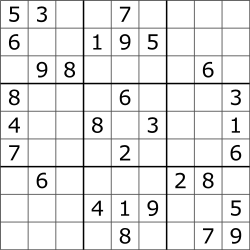
\includegraphics[width=2.5in]{../Pictures/wiki_sudoku.png}
\end{center}

There are many ways to solve such puzzles, some of which are described in:
\wwwurl{https://norvig.com/sudoku.html}


\begin{exercise}
\label{ex:sudoku1}

Using the simple ADT framework provided and the constraint propagation
approach described above, write a program that can solve ``easy'' puzzles.
The constraint propagation approach cannot completely solve ``hard''
puzzles.  A basic ADT is provided for you
in \verb^sudoku.h^, along with a simple test file
\verb^testsudoku.c^.
Write \verb^Fixed/fixed.c^
and \verb^Fixed/specific.h^, so that:

{\small
\begin{terminaloutput}
% make run
Basic Sudoku Tests ... Start
Basic Sudoku Tests ... Stop
Basic Sudoku Tests ... Start
Basic Sudoku Tests ... Stop
\end{terminaloutput}
}
\noindent works correctly. 

\noindent The code will hardwire the grid to be a fixed size $2D$~array,
and be capable of reading in the different files present in \verb^Data/Sudoku^.
Submit a single \verb^.zip^ file which contains your entire submission,
including \verb^Fixed/fixed.c^ and \verb^Fixed/specific.h^.
\end{exercise}

\begin{exercise}
\label{ex:sudoku2}

Extend your program so that all grids are solvable, even the ``hard''
examples given. One typical way to do this is to make a guess for a
square, and then backtrack to undo this if it leads to an incorrect
solution when using constraint propagation.
Efficiency of your solution is not a concern here - focus on creating
beautifully crafted (and tested) code.

\noindent Submit a single \verb^.zip^ file which contains your entire
submission, including the updated versions of \verb^Fixed/fixed.c^
and \verb^Fixed/specific.h^ in addition to \verb^solution.txt^ which
briefly describes the algorithm used.

\end{exercise}

\begin{exercise}
\label{ex:sudoku3}

Extend your program in a manner of your own choosing - this could be a
faster approach to solving all grids (but maybe at the expense of code
readability), exploring Sudokus larger than $9x9$, or allowing better
I/O or user-interaction.

\noindent Submit a single \verb^.zip^ file which contains your entire
submission, including the updated versions of \verb^Fixed/fixed.c^ and
\verb^Fixed/specific.h^ in addition to \verb^extend.txt^ which briefly
describes what you have done.

\end{exercise}



\nsection{Polymorphic Hashing}

Polymorphism is the concept of writing functions (or ADTs), without
needing to specify which particular type is being used/stored. To
understand the quicksort algorithm, for instance, doesn't really require
you to know whether you're using integers, doubles or some other type. C
is not very good at dealing with polymorphism - you'd need something
like Java or C++ for that. However, it does allow the use of
\verb^void*^ pointers for us to approximate it.

\begin{exercise}
\label{ex:hahspoly}
Here we write an implementation of a polymorphic associative array using
hashing, see \verb^assoc.h^. Both the key \& data to be used by the hash
function are of
unknown types, so we will simply store void pointers to
both of these, and the user of the associative array (and {\bf not} the
ADT itself) will be responsible for creating and maintaining such memory,
and also ensuring it doesn't change when in use by the associative array.
In the \verb^testassoc.c^ file we show two uses for such a type :
a simple string example (to find the longest word in English that is
also a valid (but different) word when spelled backwards), and a simple
integer example where we keep a record of how many unique random numbers
in a range are chosen.

Since we do not know {\bf what} the type of the key is, we
need to be careful when comparing or copying keys. Therefore, in the
\verb^assoc_init(int keysize)^ function, the user has to pass the size of the
key used (e.g. \verb^sizeof(int)^) or in the case or strings, the special value $0$.
Now we can use \verb^memcmp()^ and \verb^memcpy()^, or in the case of strings, \verb^strcmp()^
and \verb^strcpy()^ for dealing with the keys. In the case of data, the ADT only ever needs
to return a pointer to the data (not process it) via
\verb^assoc_lookup()^, so its size is not important.

Your hash table used to implement the ADT should be resizeable, and you may use
open-addressing/double-hashing or separate chaining to deal with collisions. Make no assumptions about
the maximum size of the array, and make the initial size of the array small e.g. $16$ or $17$
(a prime is useful if you're double hashing)..
You can use any hash function you wish, but if it's off the internet (etc.) cite
the source in a comment..

Submit a single \verb^assoc.zip^ file containing your code.
Your standard submission will contain the directory structure, including the two files:\\
\verb^Realloc/specific.h^ and \verb^Realloc/realloc.c^.
I will use my \verb^assoc.mk^ Makefile to compile your code,
so check that it works correctly.
\end{exercise}

Hint : when you do a resize you cannot simply
copy the old table, but must rehash your data, one entry at a time,
into the new table.  This is because your hash function is based on the
table size, and if the table size has changed you will be hashing keys
into different locations.


\nsection{MultiValue Maps}

Many data types concern a single value (e.g. a hash table), so that
a string (say) acts as both the key (by which we search for the data)
and also as the object we need to store (the value). An example of this a spelling checker,
where one word is stored (and searched for) at a time.  However, sometimes
there is a need to store a value based on a particular key - for instance
an associative array in Python allows you to perform operations such as :
\begin{codesnippet} 
population["Bristol"] = 536000
\end{codesnippet} 
where a value (the number 536000) is stored using the key (the string "Bristol").
One decision you need to make when designing such a data type is whether
multiple values are allowed for the same key; in the above example this
would make no sense - Bristol can only have one population size. But if
you wanted to store people as the key, with their salary as the value,
you might need to use a MultiValue Map (MVM) since people can have more than
one job.

Here we write the abstract type for a MultiValueMap that stores key-value pairs,
where both the key and the value are strings.

\begin{exercise}
\label{ex:mvm}
The definition of an MVM ADT is given in \verb^mvm.h^, and a file to test it is given
in \verb^testmvm.c^.  Write \verb^mvm.c^, so that:
{\small
\begin{terminaloutput}
% make -f mvm_adt.mk 
./testmvm
Basic MVM Tests ... Start
Basic MVM Tests ... Stop
\end{terminaloutput}
}
\noindent works correctly. Use a simple linked list for this, inserting
new items at the head of the list.
Make no changes to any of my files.

Submit : \verb^mvm.c^.
\end{exercise}

\nsection{Rhymes}

In the usual place is a dictionary which, for every word, lists the
phonemes (a code for a distinct unit of sound) used to pronounce that word
in American English. In this file the word itself, and its phonemes,
are separated by a `\#').  For instance:
\begin{codesnippet}
BOY#B OY1
\end{codesnippet}
shows that the word \verb^BOY^ has two phonemes : \verb^B^ and \verb^OY1^.

A simple attempt at finding rhymes for boy would match every word that has \verb^OY1^
as its final phoneme. This gives you:
\begin{terminaloutput}
POLLOI MCVOY LAFOY ALROY ILLINOIS CROIX DECOY REDEPLOY CLOY
LAVOY MOYE LOYE STOY PLOY KNOY EMPLOY ELROY JOY COY LACROIX
DEVROY ENJOY LOY COYE FOYE MOY DOI BROY TOY LABOY ROI HOY
ROYE NEU CROY SOY YOY MCCOY CHOY GOY ROY BOLSHOI MALLOY JOYE
DESTROY DELACROIX(1) DEBOY MCROY CHOI UNDEREMPLOY FLOY MCKOY
TOYE AHOY BOY OYE SGROI FOIE(1) TROY DEPLOY SAVOY UNEMPLOY
SCHEU WOY BOYE HOYE FOY OI HOI KROY EMPLOY(1) FLOURNOY OIE
MCCLOY ANNOY OY DEJOY
\end{terminaloutput}

Using two phonemes to do the matching is too many,
since the only matches are for words that have exactly the same pronunciation: 
\begin{terminaloutput}
LABOY DEBOY BOY BOYE
\end{terminaloutput}
which are not really rhymes, but homophones. Therefore, using
the {\bf correct} number of phonemes will be key to finding
`good' rhyming words.

Here we will use the MutliValue Map written in Exercise~\ref{ex:mvm} to
create two maps.  An MVM \verb^map1^ stores the word (as the key) and its final
$n$ phonemes as a single string (the value).  Now \verb^map2^ stores the
word (value), keyed by its final $n$ phonemes as a single string.
Looking up the phonemes associated with a word can be done using
the word as a key
\footnote{Strictly speaking, we don't need the
$map1$ to be capable of storing multiple values, since every word
in the dictionary is unique. We'll use it here though for simplicity.}
(via \verb^map1^), and looking up a word given its phonemes can be
achieved using \verb^map2^.

\begin{exercise}
\label{ex:rhymes}
Read in the dictionary, and for each line
in turn, store the data in the two maps.  Now for a requested word to be
`rhymed', search for its phonemes using \verb^map1^ and then search for
matching words using \verb^map2^. The number of phonemes specified for
this rhyming is given via the command line, as are the words to be rhymed:
\begin{terminaloutput}
$ ./homophones -n 3 RHYME
RHYME (R AY1 M): PRIME RHYME ANTICRIME(1) CRIME ANTICRIME
GRIME RIME
\end{terminaloutput}
The \verb^-n^ flag specifies the number of phonemes to use (you may
assume the number associated with it always is always separated from
the flag by a space).  If no \verb^-n^ flag is given then the value $3$
is assumed.  It only makes sense to use a value of $n \leq$ the number of
phonemes in the two words being checked. If you use a value greater than this,
the results are undefined.

The list of words to be matched may be found on the command line:
\begin{terminaloutput}
$ ./homophones -n 4 CHRISTMAS PROGRAM PASSING
CHRISTMAS (S M AH0 S): ISTHMUS CHRISTMAS CHRISTMAS'
PROGRAM (G R AE2 M): CENTIGRAM ENGRAM HISTOGRAM WOLFGRAM
MONOGRAM LOGOGRAM HOLOGRAM MICROGRAM SONOGRAM ANGIOGRAM
TELEGRAM PROGRAMME ELECTROCARDIOGRAM ELECTROPHORETOGRAM
REPROGRAM MILLIGRAM ANAGRAM PEGRAM POLYGRAM DIAGRAM
EPIGRAM PROGRAM MAILGRAM MILGRAM INGHRAM CABLEGRAM
MAMMOGRAM KILOGRAM
PASSING (AE1 S IH0 NG): GASSING MASENG SURPASSING KASSING
HASSING PASSING AMASSING MASSING CLASSING HARASSING
\end{terminaloutput}
Use the Makefile supplied for this task. Make the output as similar to that shown above as possible.

Submit : \verb^homophones.c^.
\end{exercise}

\nsection{Faster MVMs}
The ADT for MVMs used in Exercise~\ref{ex:mvm} is a simple linked list -
insertion is fast, but searching is slow.

\begin{exercise}
Write a new version of this MVM ADT called \verb^fmvm.c^ that
implements exactly the same functionality but has a faster search time.
The file \verb^fmvm.h^ will change very little from \verb^mvm.h^, with maybe
only the structures changing, but not the function prototypes.  A similar
testing file to that used previously, now called \verb^testfmvm.c^
should also be written.  Note that any ordering of data when using
the \verb^mvm_print^ and \verb^mvm_multisearch^ functions is acceptable,
so these can't be tested in exactly the same manner.

By simply changing the \verb^#include^ from \verb^<mvm.h>^ to \verb^<fmvm.h>^
in your \verb^homephones.c^ file from Exercise~\ref{ex:rhymes}, and compiling it against
\verb^fmvm.c^, I can test that program works identically.

Make it clear what you have done to speed up your searching (and how)
using comments at the top of \verb^fmvm.h^

Submit : \verb^fmvm.c^, \verb^fmvm.h^ and \verb^testfmvm.c^
\end{exercise}


\newcommand{\bb}{white}
\newcommand{\ff}{black}

\newcommand{\sixel}[6]{%
\begin{tikzpicture}[scale=0.333, every node/.style={scale=0.333}]
\matrix[sixelstyle]
{
|[fill=#1]| \& |[fill=#2]| \\
|[fill=#3]| \& |[fill=#4]| \\
|[fill=#5]| \& |[fill=#6]| \\
};
\end{tikzpicture}%
}

\newcommand{\sepsix}[6]{%
\begin{tikzpicture}[scale=0.333, every node/.style={scale=0.333}]
\matrix[sepsixstyle]
{
|[fill=#1]| \& |[fill=#2]| \\
|[fill=#3]| \& |[fill=#4]| \\
|[fill=#5]| \& |[fill=#6]| \\
};
\end{tikzpicture}%
}

%\chapterimage{../Pictures/teletext_wk12.pdf}
\chapterimage{../Pictures/ttl2.jpg}
\chapter{Parsing Data}

\tikzset{word ladder/.style={
  matrix of nodes
  , execute at empty cell={\node[draw=gray,text=gray,fill=white]{0};}
  , nodes in empty cells=false
  , nodes={shape=rectangle, draw=none,fill=none,text=black,minimum width=0.6cm,minimum height=0.35cm,outer sep=0pt,align=center,inner sep=0pt,font=\small}
  , row sep={0.35cm,between origins}
  , column sep={0.6cm,between origins}
},
}

\tikzset{spacehash board/.style={
  matrix of nodes
  , execute at empty cell={\node[draw=gray,text=gray,fill=white]{ };}
  , nodes in empty cells=false
  , nodes={draw=gray,fill=ocre,text=gray,text depth=0.5ex,text height=2ex,text width=1em,outer sep=0pt,align=center,inner sep=0pt}
  , row sep={#1,between origins}
  , column sep={#1,between origins}
},
}

\tikzset{noughtsone board/.style={
  matrix of nodes
  , execute at empty cell={\node[draw=gray,text=gray,fill=white]{0};}
  , nodes in empty cells=false
  , nodes={draw=gray,fill=ocre,text=gray,minimum width=#1,minimum height=#1,outer sep=0pt,align=center,inner sep=0pt}
  , row sep={#1,between origins}
  , column sep={#1,between origins}
},
  noughtsone board/.default=0.5cm
}

\tikzset{twocolour board/.style={
  matrix of nodes
  , execute at empty cell={\node[text=white,fill=white]{+};}
  , nodes in empty cells=false
  , nodes={draw=gray,fill=ocre,minimum width=#1,minimum height=#1,outer sep=0pt,align=center,inner sep=0pt,font=\tiny}
  , text=ocre
  , row sep={#1,between origins}
  , column sep={#1,between origins}
},
  twocolour board/.default=0.5cm
}
\tikzset{twocolour board/.style={
  matrix of nodes
  , execute at empty cell={\node[text=white,fill=white]{+};}
  , nodes in empty cells=false
  , nodes={draw=gray,fill=ocre,minimum width=#1,minimum height=#1,outer sep=0pt,align=center,inner sep=0pt,font=\tiny}
  , text=ocre
  , row sep={#1,between origins}
  , column sep={#1,between origins}
},
  twocolour board/.default=0.5cm
}

%% Candy Crush-style games, colour & label
\tikzset{crushstyle board/.style={
  matrix of nodes
  , nodes={draw=gray,fill=ocre,minimum width=#1,minimum height=#1,outer sep=0pt,align=center,inner sep=0pt,font=\tiny}
  , text=ocre
  , row sep={#1,between origins}
  , column sep={#1,between origins}
},
  crushstyle board/.default=0.5cm
}

%% WaTor-style games, colour & label
\tikzset{watorstyle board/.style={
  matrix of nodes
  , nodes={fill=cyan,minimum width=#1,minimum height=#1,outer sep=0pt,align=center,inner sep=0pt,font=\tiny}
  , text=black
  , row sep={#1,between origins}
  , column sep={#1,between origins}
},
  watorstyle board/.default=0.25cm
}

%% 8-tile style
\tikzset{eighttilestyle board/.style={
  matrix of nodes, ampersand replacement={\&}
  , execute at empty cell={\node[draw=gray,text=gray,fill=gray]{0};}
  , nodes={fill=gray,minimum width=#1,minimum height=#1,outer sep=0pt,align=center,inner sep=0pt,font=\tiny}
  , text=ocre
  , row sep={#1,between origins}
  , column sep={#1,between origins}
},
  eighttilestyle board/.default=0.25cm
}

\tikzset{sixelstyle/.style={
  matrix of nodes, ampersand replacement={\&}
  , nodes={draw=black,fill=gray,text=gray
     %,minimum height=1pt, minimum width=1pt
     %,row sep=1pt, column sep=1pt
}
},
   sixelstyle/.default=0.3em
}

\tikzset{sepsixstyle/.style={
  matrix of nodes, ampersand replacement={\&}
  , nodes={draw=white,fill=gray,text=gray,
     minimum height=1pt, minimum width=1pt,
     row sep=1pt, column sep=1pt}
},
   sixelstyle/.default=0.3em
}


\nsection{Teletext}

In the early 1970s, Phillips Labs began work on transmitting digital
information across the television network. The aim was to
provide up-to-date news and weather information via a television set. 
This system was trialled first by the BBC in a system that eventually became
known as ``Ceefax'' and then on other independant British terrestrial stations as ``Oracle''.
A very similar system was implemented on the BBC microcomputer, known as {\it Mode 7}.
\begin{figure}[ht]
\centering{
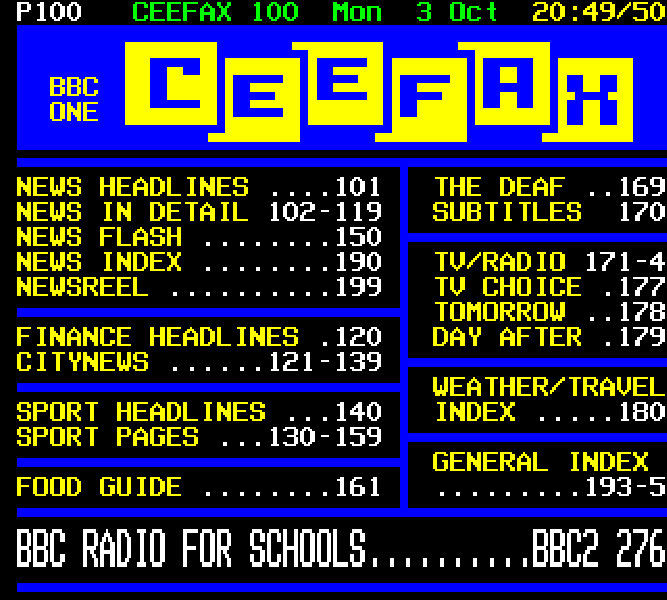
\includegraphics{../Pictures/teletext100.pdf}
}
\caption{An example Ceefax page circa 1983. Taken from {\tt http://teletext.mb21.co.uk/gallery/ceefax/main1.shtml}}
\label{fig:tt100}
\end{figure}
An example of such a Ceefax screen is shown in Figure~\ref{fig:tt100}.

This project, inspired by such teletext systems, will allow a $40 \times 25$ ($1000$) character
file to be rendered to the screen, using similar control codes. However, some control
codes are not implemented, including those to do with flashing or hidden text, and transparent backgrounds. In particular, our definition of the {\it double height} control code differs from that of
the traditional one.

\subsection*{The Control Codes}

This section is based to a large extent to Richard Russell's description of
Mode 7 on the BBC Micro:
\verb^http://www.bbcbasic.co.uk/tccgen/manual/tcgen2.html^.

\begin{table}
\begin{tabular}{|c|c|c|c|c|c|c|c|c|}\hline
   &0x8            & 0x9               & 0xA&0xB&0xC& 0xD         &0xE& 0xF         \\
 0 &Unused/Reserved&Unused/Reserved    &    & 0 & @ & P           & - & p           \\
 1 &Red Alphanumeric       &Red Graphics       & !  & 1 & A & Q           & a & q           \\
 2 &Green Alphanumeric     &Green Graphics     & "  & 2 & B & R           & b & r           \\
 3 &Yellow Alphanumeric    &Yellow Graphics    & $\pounds$  & 3 & C & S           & c & s           \\
 4 &Blue   Alphanumeric    &Blue   Graphics    & \$ & 4 & D & T           & d & t           \\
 5 &Magenta Alphanumeric   &Magenta Graphics   & \% & 5 & E & U           & e & u           \\
 6 &Cyan Alphanumeric      &Cyan Graphics      & \& & 6 & F & V           & f & v           \\
 7 &White Alphanumeric     &White Graphics     &  ' & 7 & G & W           & g & w           \\
 8 &Unused/Reserved&Unused/Reserved    &  ( & 8 & H & X           & h & x           \\
 9 &Unused/Reserved&Contiguous Graphics&  ) & 9 & I & Y           & i & y           \\
 A &Unused/Reserved&Separated Graphics &  * & : & J & Z           & j & z           \\
 B &Unused/Reserved&Unused/Reserved    &  + & ; & K & $\leftarrow$& k &$\sfrac{1}{4}$\\
 C &Single Height  &Black Background   &  , & < & L &$\sfrac{1}{2}$& l & $||$           \\
 D &Double Height  &New Background     &  - & = & M &$\rightarrow$ & m &$\sfrac{3}{4}$\\
 E &Unused/Reserved&Hold Graphics      &  . & > & N & $\uparrow$  & n &$\div$    \\
 F &Unused/Reserved&Release Graphics   &  / & ? & O & \#           & o & \textblock           \\ \hline
\end{tabular}
\caption{The control codes and characters for alphanumeric mode. Note here (because we're using white paper) foreground is shown in black and background in white. On a teletext screen we use white on a black background.}
\label{tab:normgraph}
\end{table}

\begin{table}
\begin{tabular}{|c|c|c|c|c|c|c|c|c|}\hline
   &0x8            & 0x9               		& 0xA&0xB&0xC& 0xD         &0xE& 0xF         \\
 0 &Unused/Reserved&Unused/Reserved    		& \sixel{\bb}{\bb}{\bb}{\bb}{\bb}{\bb} & \sixel{\bb}{\bb}{\bb}{\bb}{\ff}{\bb} & @ & P           & \sixel{\bb}{\bb}{\bb}{\bb}{\bb}{\ff} & \sixel{\bb}{\bb}{\bb}{\bb}{\ff}{\ff}\\
 1 &Red Alphanumeric       &Red Graphics	& \sixel{\ff}{\bb}{\bb}{\bb}{\bb}{\bb} & \sixel{\ff}{\bb}{\bb}{\bb}{\ff}{\bb} & A & Q           & \sixel{\ff}{\bb}{\bb}{\bb}{\bb}{\ff} & \sixel{\ff}{\bb}{\bb}{\bb}{\ff}{\ff}\\
 2 &Green Alphanumeric     &Green Graphics	& \sixel{\bb}{\ff}{\bb}{\bb}{\bb}{\bb} & \sixel{\bb}{\ff}{\bb}{\bb}{\ff}{\bb} & B & R           & \sixel{\bb}{\ff}{\bb}{\bb}{\bb}{\ff} & \sixel{\bb}{\ff}{\bb}{\bb}{\ff}{\ff}\\
 3 &Yellow Alphanumeric    &Yellow Graphics	& \sixel{\ff}{\ff}{\bb}{\bb}{\bb}{\bb} & \sixel{\ff}{\ff}{\bb}{\bb}{\ff}{\bb} & C & S           & \sixel{\ff}{\ff}{\bb}{\bb}{\bb}{\ff} & \sixel{\ff}{\ff}{\bb}{\bb}{\ff}{\ff}\\
 4 &Blue   Alphanumeric    &Blue   Graphics	& \sixel{\bb}{\bb}{\ff}{\bb}{\bb}{\bb} & \sixel{\bb}{\bb}{\ff}{\bb}{\ff}{\bb} & D & T           & \sixel{\bb}{\bb}{\ff}{\bb}{\bb}{\ff} & \sixel{\bb}{\bb}{\ff}{\bb}{\ff}{\ff}\\
 5 &Magenta Alphanumeric   &Magenta Graphics	& \sixel{\ff}{\bb}{\ff}{\bb}{\bb}{\bb} & \sixel{\ff}{\bb}{\ff}{\bb}{\ff}{\bb} & E & U           & \sixel{\ff}{\bb}{\ff}{\bb}{\bb}{\ff} & \sixel{\ff}{\bb}{\ff}{\bb}{\ff}{\ff}\\
 6 &Cyan Alphanumeric      &Cyan Graphics	& \sixel{\bb}{\ff}{\ff}{\bb}{\bb}{\bb} & \sixel{\bb}{\ff}{\ff}{\bb}{\ff}{\bb} & F & V           & \sixel{\bb}{\ff}{\ff}{\bb}{\bb}{\ff} & \sixel{\bb}{\ff}{\ff}{\bb}{\ff}{\ff}\\
 7 &White Alphanumeric     &White Graphics	& \sixel{\ff}{\ff}{\ff}{\bb}{\bb}{\bb} & \sixel{\ff}{\ff}{\ff}{\bb}{\ff}{\bb} & G & W           & \sixel{\ff}{\ff}{\ff}{\bb}{\bb}{\ff} & \sixel{\ff}{\ff}{\ff}{\bb}{\ff}{\ff}\\
 8 &Unused/Reserved&Unused/Reserved		& \sixel{\bb}{\bb}{\bb}{\ff}{\bb}{\bb} & \sixel{\bb}{\bb}{\bb}{\ff}{\ff}{\bb} & H & X           & \sixel{\bb}{\bb}{\bb}{\ff}{\bb}{\ff} & \sixel{\bb}{\bb}{\bb}{\ff}{\ff}{\ff}\\
 9 &Unused/Reserved&Contiguous Graphics		& \sixel{\ff}{\bb}{\bb}{\ff}{\bb}{\bb} & \sixel{\ff}{\bb}{\bb}{\ff}{\ff}{\bb} & I & Y           & \sixel{\ff}{\bb}{\bb}{\ff}{\bb}{\ff} & \sixel{\ff}{\bb}{\bb}{\ff}{\ff}{\ff}\\
 A &Unused/Reserved&Separated Graphics		& \sixel{\bb}{\ff}{\bb}{\ff}{\bb}{\bb} & \sixel{\bb}{\ff}{\bb}{\ff}{\ff}{\bb} & J & Z           & \sixel{\bb}{\ff}{\bb}{\ff}{\bb}{\ff} & \sixel{\bb}{\ff}{\bb}{\ff}{\ff}{\ff}\\
 B &Unused/Reserved&Unused/Reserved		& \sixel{\ff}{\ff}{\bb}{\ff}{\bb}{\bb} & \sixel{\ff}{\ff}{\bb}{\ff}{\ff}{\bb} & K & $\leftarrow$& \sixel{\ff}{\ff}{\bb}{\ff}{\bb}{\ff} & \sixel{\ff}{\ff}{\bb}{\ff}{\ff}{\ff}\\
 C &Single Height  &Black Background		& \sixel{\bb}{\bb}{\ff}{\ff}{\bb}{\bb} & \sixel{\bb}{\bb}{\ff}{\ff}{\ff}{\bb} & L &$\sfrac{1}{2}$& \sixel{\bb}{\bb}{\ff}{\ff}{\bb}{\ff} & \sixel{\bb}{\bb}{\ff}{\ff}{\ff}{\ff}\\
 D &Double Height  &New Background		& \sixel{\ff}{\bb}{\ff}{\ff}{\bb}{\bb} & \sixel{\ff}{\bb}{\ff}{\ff}{\ff}{\bb} & M &$\rightarrow$ & \sixel{\ff}{\bb}{\ff}{\ff}{\bb}{\ff} & \sixel{\ff}{\bb}{\ff}{\ff}{\ff}{\ff}\\
 E &Unused/Reserved&Hold Graphics		& \sixel{\bb}{\ff}{\ff}{\ff}{\bb}{\bb} & \sixel{\bb}{\ff}{\ff}{\ff}{\ff}{\bb} & N & $\uparrow$  & \sixel{\bb}{\ff}{\ff}{\ff}{\bb}{\ff} & \sixel{\bb}{\ff}{\ff}{\ff}{\ff}{\ff}\\
 F &Unused/Reserved&Release Graphics		& \sixel{\ff}{\ff}{\ff}{\ff}{\bb}{\bb} & \sixel{\ff}{\ff}{\ff}{\ff}{\ff}{\bb} & O & \#           & \sixel{\ff}{\ff}{\ff}{\ff}{\bb}{\ff} & \sixel{\ff}{\ff}{\ff}{\ff}{\ff}{\ff}\\ \hline
\end{tabular}
\caption{The control codes and characters for contiguous graphics mode.}
\label{tab:contgraph}
\end{table}

\begin{table}
\begin{tabular}{|c|c|c|c|c|c|c|c|c|}\hline
   &0x8            & 0x9               		& 0xA&0xB&0xC& 0xD         &0xE& 0xF         \\
 0 &Unused/Reserved&Unused/Reserved    		& \sepsix{\bb}{\bb}{\bb}{\bb}{\bb}{\bb} & \sepsix{\bb}{\bb}{\bb}{\bb}{\ff}{\bb} & @ & P           & \sepsix{\bb}{\bb}{\bb}{\bb}{\bb}{\ff} & \sepsix{\bb}{\bb}{\bb}{\bb}{\ff}{\ff}\\
 1 &Red Alphanumeric       &Red Graphics	& \sepsix{\ff}{\bb}{\bb}{\bb}{\bb}{\bb} & \sepsix{\ff}{\bb}{\bb}{\bb}{\ff}{\bb} & A & Q           & \sepsix{\ff}{\bb}{\bb}{\bb}{\bb}{\ff} & \sepsix{\ff}{\bb}{\bb}{\bb}{\ff}{\ff}\\
 2 &Green Alphanumeric     &Green Graphics	& \sepsix{\bb}{\ff}{\bb}{\bb}{\bb}{\bb} & \sepsix{\bb}{\ff}{\bb}{\bb}{\ff}{\bb} & B & R           & \sepsix{\bb}{\ff}{\bb}{\bb}{\bb}{\ff} & \sepsix{\bb}{\ff}{\bb}{\bb}{\ff}{\ff}\\
 3 &Yellow Alphanumeric    &Yellow Graphics	& \sepsix{\ff}{\ff}{\bb}{\bb}{\bb}{\bb} & \sepsix{\ff}{\ff}{\bb}{\bb}{\ff}{\bb} & C & S           & \sepsix{\ff}{\ff}{\bb}{\bb}{\bb}{\ff} & \sepsix{\ff}{\ff}{\bb}{\bb}{\ff}{\ff}\\
 4 &Blue   Alphanumeric    &Blue   Graphics	& \sepsix{\bb}{\bb}{\ff}{\bb}{\bb}{\bb} & \sepsix{\bb}{\bb}{\ff}{\bb}{\ff}{\bb} & D & T           & \sepsix{\bb}{\bb}{\ff}{\bb}{\bb}{\ff} & \sepsix{\bb}{\bb}{\ff}{\bb}{\ff}{\ff}\\
 5 &Magenta Alphanumeric   &Magenta Graphics	& \sepsix{\ff}{\bb}{\ff}{\bb}{\bb}{\bb} & \sepsix{\ff}{\bb}{\ff}{\bb}{\ff}{\bb} & E & U           & \sepsix{\ff}{\bb}{\ff}{\bb}{\bb}{\ff} & \sepsix{\ff}{\bb}{\ff}{\bb}{\ff}{\ff}\\
 6 &Cyan Alphanumeric      &Cyan Graphics	& \sepsix{\bb}{\ff}{\ff}{\bb}{\bb}{\bb} & \sepsix{\bb}{\ff}{\ff}{\bb}{\ff}{\bb} & F & V           & \sepsix{\bb}{\ff}{\ff}{\bb}{\bb}{\ff} & \sepsix{\bb}{\ff}{\ff}{\bb}{\ff}{\ff}\\
 7 &White Alphanumeric     &White Graphics	& \sepsix{\ff}{\ff}{\ff}{\bb}{\bb}{\bb} & \sepsix{\ff}{\ff}{\ff}{\bb}{\ff}{\bb} & G & W           & \sepsix{\ff}{\ff}{\ff}{\bb}{\bb}{\ff} & \sepsix{\ff}{\ff}{\ff}{\bb}{\ff}{\ff}\\
 8 &Unused/Reserved&Unused/Reserved		& \sepsix{\bb}{\bb}{\bb}{\ff}{\bb}{\bb} & \sepsix{\bb}{\bb}{\bb}{\ff}{\ff}{\bb} & H & X           & \sepsix{\bb}{\bb}{\bb}{\ff}{\bb}{\ff} & \sepsix{\bb}{\bb}{\bb}{\ff}{\ff}{\ff}\\
 9 &Unused/Reserved&Contiguous Graphics		& \sepsix{\ff}{\bb}{\bb}{\ff}{\bb}{\bb} & \sepsix{\ff}{\bb}{\bb}{\ff}{\ff}{\bb} & I & Y           & \sepsix{\ff}{\bb}{\bb}{\ff}{\bb}{\ff} & \sepsix{\ff}{\bb}{\bb}{\ff}{\ff}{\ff}\\
 A &Unused/Reserved&Separated Graphics		& \sepsix{\bb}{\ff}{\bb}{\ff}{\bb}{\bb} & \sepsix{\bb}{\ff}{\bb}{\ff}{\ff}{\bb} & J & Z           & \sepsix{\bb}{\ff}{\bb}{\ff}{\bb}{\ff} & \sepsix{\bb}{\ff}{\bb}{\ff}{\ff}{\ff}\\
 B &Unused/Reserved&Unused/Reserved		& \sepsix{\ff}{\ff}{\bb}{\ff}{\bb}{\bb} & \sepsix{\ff}{\ff}{\bb}{\ff}{\ff}{\bb} & K & $\leftarrow$& \sepsix{\ff}{\ff}{\bb}{\ff}{\bb}{\ff} & \sepsix{\ff}{\ff}{\bb}{\ff}{\ff}{\ff}\\
 C &Single Height  &Black Background		& \sepsix{\bb}{\bb}{\ff}{\ff}{\bb}{\bb} & \sepsix{\bb}{\bb}{\ff}{\ff}{\ff}{\bb} & L &$\sfrac{1}{2}$& \sepsix{\bb}{\bb}{\ff}{\ff}{\bb}{\ff} & \sepsix{\bb}{\bb}{\ff}{\ff}{\ff}{\ff}\\
 D &Double Height  &New Background		& \sepsix{\ff}{\bb}{\ff}{\ff}{\bb}{\bb} & \sepsix{\ff}{\bb}{\ff}{\ff}{\ff}{\bb} & M &$\rightarrow$ & \sepsix{\ff}{\bb}{\ff}{\ff}{\bb}{\ff} & \sepsix{\ff}{\bb}{\ff}{\ff}{\ff}{\ff}\\
 E &Unused/Reserved&Hold Graphics		& \sepsix{\bb}{\ff}{\ff}{\ff}{\bb}{\bb} & \sepsix{\bb}{\ff}{\ff}{\ff}{\ff}{\bb} & N & $\uparrow$  & \sepsix{\bb}{\ff}{\ff}{\ff}{\bb}{\ff} & \sepsix{\bb}{\ff}{\ff}{\ff}{\ff}{\ff}\\
 F &Unused/Reserved&Release Graphics		& \sepsix{\ff}{\ff}{\ff}{\ff}{\bb}{\bb} & \sepsix{\ff}{\ff}{\ff}{\ff}{\ff}{\bb} & O & \#           & \sepsix{\ff}{\ff}{\ff}{\ff}{\bb}{\ff} & \sepsix{\ff}{\ff}{\ff}{\ff}{\ff}{\ff}\\ \hline
\end{tabular}
\caption{The control codes and characters for separated graphics mode.}
\label{tab:sepgraph}
\end{table}

\subsubsection*{Coloured Text}
By using the control codes $129 - 135$ ($0x81 - 0x87$ in hexadecimal) the rest of the line will
have text in the selected foreground colour.

To change the background colour, you issue a foreground colour code first, and then the "New Background" character. All the following line will now have the appropriate background colour.
You'll typically then need to choose a new foreground text colour.

\subsubsection*{Block Graphics}

Teletext has a very limited ability to output low-resolution block graphics. These
shapes take the place of other characters in the font and are enabled by issuing one
of the coloured graphics codes e.g. {\it red graphics}. At this point the characters
available for printing are as displayed in Table~\ref{tab:contgraph}. These new graphics
characters are made up of six smaller boxes, known as {\it sixels}. Each individual sixel has
a code, either, $1,2,4,8,16$ or $64$ as shown in Figure~\ref{fig:graphcodes}.
\begin{figure}[ht]
\begin{center}
\begin{tabular}{|c|c|}\hline
1 & 2 \\ \hline
4 & 8 \\ \hline
16 & {\bf 64} \\ \hline
\end{tabular}
\end{center}
\caption{Values for computing graphics codes, as added to the base code $160$ ($0xA0$ in hexadecimal).}
\label{fig:graphcodes}
\end{figure}
By adding these values together we can define which
of these sixels are `lit' or not. If we wish the three left-hand
ones to be lit we'd use the base code ($160$) plus $1, 4$ and $16 = 181$ ($0xB5$ in
hexadecimal).
Therefore issuing the coding {\it green graphics} and then code $181$ puts
a green vertical bar on the screen.

Notice in Table~\ref{tab:contgraph} that some other characters are still available,
particularly all capital letters. This allow simple printing of capitals, even
when in graphics mode, and is know as {\it blast-through Text}.

There is another set of block graphics, as shown in Table~\ref{tab:sepgraph}. For these,
each sixel is separated from others by thin vertical and horizontal lines. This mode is known
as {\it separated graphics} mode.

\subsubsection*{Held Graphics}

Generally all control codes are displayed as spaces, in the current
background colour. In the held graphics mode, control code $158$ ($0x9E$
in hexadecimal), control codes are instead displayed as a copy of the most
recently displayed graphics symbol. This permits a limited range of abrupt
display colour changes.  The held graphics character is displayed in the
same contiguous/separated mode as when it was first displayed. If there
has been a change in the text/graphics mode or the normal/double-height
mode since the last graphics character was displayed, the held graphics
character is cleared and control codes once again display as spaces.

To switch held graphics mode off, use the {\it release graphics} control code.

\subsubsection*{Double Height}

By using the {\it double height} control code, characters are displayed as twice their
normal size. Since they span two lines, the control codes and characters
have to be repeated on the next line too, for them to be correctly displayed.
The rule here, is that if a character is to be displayed as double height, the top half
of the character is displayed on the first line, and the bottom half on the next line.
The bottom half is only displayed as double height if the character vertically above it was
also displayed in {\it double height} mode. The character in question need not be the same one.

Note: here we deviate from other definitions of this control code.

\subsubsection*{Some General Guidelines}

\begin{itemize}
\item Characters are considered 7-bit (the 8th bit was typically used for parity
checking over the noisy television signal). Therefore any character less
than $128 (0x80)$ should have $128$ added to it. For, example if you
read in character  $32$ (space), it should be `converted' to character $160$.
\item Each newline on the Teletext page automatically begins with
White text, single height, contiguous graphics, black background, release graphics.
\item With the the exception of {\it hold graphics} (see above), control characters are generally rendered in the same manner as a space would
be. If the background is currently red and text colour yellow, say, then the control code would show as an empty red background.
\end{itemize}


\begin{exercise}
Implement a teletext rendering system. The $1000$ character input
file should be read in using \verb^argv[1]^.

There are many ambiguities
as to how various sequences of codes should be rendered. To help with
this, several example files have been posted on the unit web page. 
If there is still doubt, make a best-guess and state your assumptions
in the code.

Submit the testing you have undertaken, including examples and a description
of your strategies. This should convince us that you have tested every line
of code, and that it works correctly. If there are still issues/bugs state
them clearly. Also, point out any bugs that you have successfully found using
these approaches. Submit a file named \verb^testing.txt^, along with any other
files you feel necessary in the appropriate directory.

No particular strategy is mandated. You may wish to explore a couple and briefly
discuss strengths and weaknesses. 

Undertake an extension of your choosing. Examples of these include:
\begin{itemize}
\item A system that allows you to quickly author teletext pages (perhaps
using a recursive-descent parser?)
\item Automatic image to teletext conversion.
\item Automatic (simple) html to teletext conversion (and/or vice-versa).
\end{itemize}
Remember, that the assessment is based on the quality of your coding, so choose
something to demonstrate an aspect of programming or software engineering
that you haven't had a chance to use in the main assignment. Submit a file named
\verb^extension.txt^ outlining, in brief, your contribution. 

\subsection*{Hints}

\begin{itemize}
\item Don't add graphics too early - the
code is easier to test and debug with textual output to begin with.
\item I advise you to use SDL for your graphics output. The library provided previously contained
two functions to deal with printing characters~: \verb^Neill_SDL_ReadFont()^ and
\verb^Neill_SDL_DrawString()^. The font file \verb^m7fixed.fnt^ provides the basic
characters required here, but not the sixels. By understanding how the font data
is rendered, the double height version of the characters should be relatively simple.
\item Don't try to do all aspects of this at once - begin with coloured characters only. Add more
advanced functionality later.
\item Plan how you are going to store your data early in the design process.
Does each character need its own data structure? Does each line? Can this be abstracted?
\end{itemize}

Please create a directory structure, so that I can easily find the
different subsections.  Your testing strategy will be explained in
\verb^testing.txt^, and your extension as \verb^extension.txt^. For
the source and extension sections, make sure there's a
\verb^Makefile^, so that I can easily build the code.

\begin{verbatim}
            ------Top Directory------
            |            |          |           
            |            |          |           
            |            |          |            
            |            |          |             
          source      testing    extension   
            |            |          |
           ...          ...   extension.txt
           ...          ...       ...
         Makefile     Makefile    ...  
                    testing.txt
\end{verbatim}

Bundle all of these up as one {\bf single} \verb^.zip^ submission -
not one for each subsection.
\end{exercise}

\nsection{Guido van Robot}

\begin{center}
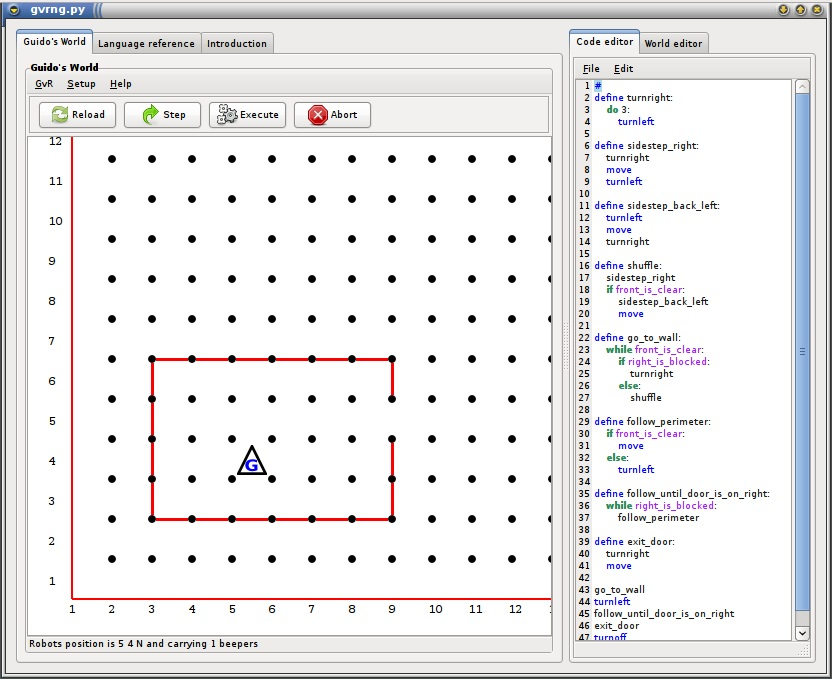
\includegraphics[scale=0.75]{./gnuLinuxGvR.jpg}
\end{center}

From \wwwurl{http://gvr.sourceforge.net/}
{\small
\begin{quote}
Guido van Robot can face in one of four directions, north, east, south, and west. He turns only 90 degrees at a time, so he can't face northeast, for instance. In Guido's world, streets run east-west, and are numbered starting at 1. There are no zero or negative street numbers. Avenues run north-south, and are also numbered starting at 1, with no zero or negative avenue numbers. At the intersection of a street and avenue is a corner. Guido moves from one corner to to the next in a single movement. Because he can only face in one of four directions, when he moves he changes his location by one avenue, or by one street, but not both!
\end{quote}
}

\subsection*{Simple .wld File}

\begin{verbatim}
Robot 5 4 N 1
Wall 3 2 N 6
Wall 2 3 E 4
Wall 3 6 N 6
Wall 8 3 E 2
Wall 8 6 E
\end{verbatim}
\begin{center}
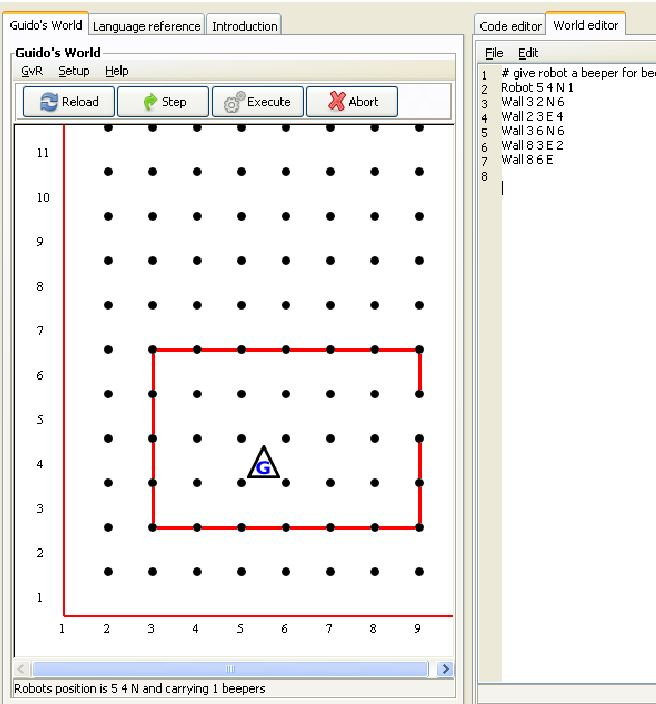
\includegraphics[scale=0.5]{../Pictures/GvRsimple1.jpg}
\end{center}

\subsection*{\bf Simple .gvr File}
\begin{verbatim}
move
move
move
move
turnoff
\end{verbatim}
\begin{center}
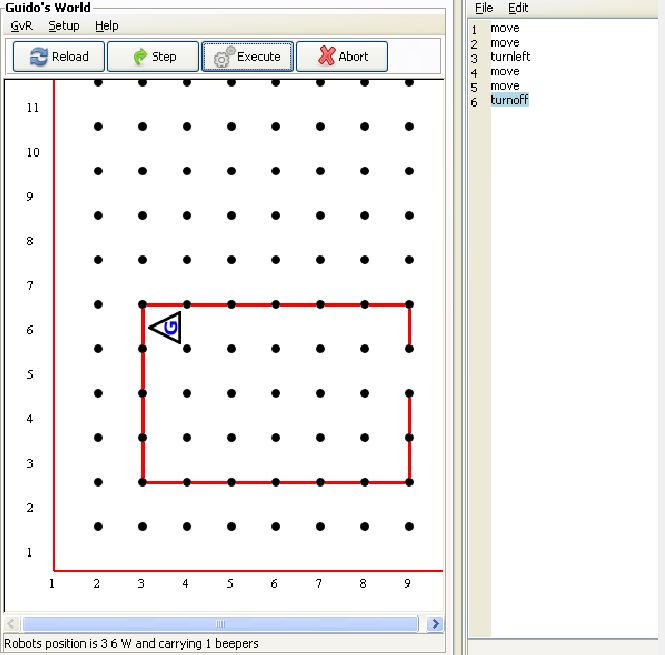
\includegraphics[scale=0.5]{./GvRsimple2.jpg}
\end{center}


\subsection*{Do Loops}
\begin{verbatim}
do 2 :
   putbeeper
   move
turnoff
\end{verbatim}

\subsection*{Conditional Loop}
\begin{verbatim}
while front_is_clear :
   putbeeper
   move
turnoff
\end{verbatim}

\subsection*{Branching}
\begin{verbatim}
do 13 :
   if front_is_clear :
      putbeeper
      move
   else :
      turnleft
turnoff
\end{verbatim}

\subsection*{The Formal Grammar}
{\small
\begin{verbatim}
<PROGRAM>   ::= <BLOCK>
<BLOCK>     ::= "turnoff" |
                "move" <BLOCK> |
                "turnleft" <BLOCK> |
                "pickbeeper" <BLOCK> |
                "putbeeper" <BLOCK> |
                <DO> <BLOCK> |
                <WHILE> <BLOCK> |
                <IF> <BLOCK>
<DO>        ::= "do" <num> ":"
                   <BLOCK>
<WHILE>     ::= "while" <TEST> ":"
                   <BLOCK>
<IF>        ::= "if" <TEST> ":"
                   <BLOCK> |
              "if" <TEST> ":"
                   <BLOCK>
              "else" ":"
                   <BLOCK>
<TEST>      ::= <WALL> | <BEEP> | <COMPASS>
\end{verbatim}
}

{\small
\begin{verbatim}
<WALL>      ::= "front_is_clear" |
                "front_is_blocked" |
                "left_is_clear" |
                "left_is_blocked" |
                "right_is_clear" |
                "right_is_blocked"
<BEEP>      ::= "next_to_a_beeper" |
                "not_next_to_a_beeper" |
                "any_beepers_in_beeper_bag" |
                "no_beepers_in_beeper_bag"
<COMPASS>   ::= "facing_north" |
                "not_facing_north" |
                "facing_south" |
                "not_facing_south" |
                "facing_east" |
                "not_facing_east" |
                "facing_west" |
                "not_facing_west"
\end{verbatim}
}

This ignores some Guido instructions, e.g. \verb^elseif^
and \verb^define^. It also doesn't well explain how to spot
the end of a \verb^DO^ etc. which is marked by a reduction in
indentation.
The definition of \verb^.wld^ files is so simple a recursive
descent parser (and hence grammar) is not required.

\begin{exercise}
\begin{itemize}

\item (25\%) To implement a recursive descent parser - this says
whether or not the given \verb^.gvr^ and \verb^.wld^ follow the formal grammar or not.
The input files are specified via \verb^argv[1]^ (\verb^.gvr^) and \verb^argv[2]^ (\verb^.wld^) .

\item (25\%) To implement an interpreter, so that the instructions are
executed. Printing the world and robot to screen
using simple characters is fine, but many will wish to use SDL.

\item (25\%) To show a testing strategy on the above -
you should give details of
white-box and black-box testing done on your code. Describe any
test-harnesses used. Give examples of the output of many different
programs. Convince me that every line of your C code
has been tested.

\item (25\%) To show an extension to the project in a direction of
your choice. It should demonstrate your understanding of some aspect
of programming or S/W engineering. If you extend the formal grammar
make sure that you show the new, full grammar.

Submit the program(s) and a Makefile so that I can:

\item Compile the parser by typing `make parse'.
\item Compile the interpreter by typing `make interp'.
\item Compile the extension by typing `make extension'.
\item Submit a test strategy report called test.txt. This will include
sample outputs, any code written especially for testing etc.
\item Submit an extension report called `extend.txt'. This is quite
brief and explains the extension attempted.

\item You need to be able to load a world file and a \verb^.gvr^
and say if they are valid of not.
\item Don't try to write the entire program in one go. Try a cut
down version of the grammar first, e.g.:
{\small
\begin{verbatim}
<PROGRAM>   ::= <BLOCK>
<BLOCK>     ::= "turnoff" |
                "move" <BLOCK> |
                "turnleft" <BLOCK> |
                "pickbeeper" <BLOCK> |
                "putbeeper" <BLOCK>
<DO>        ::= "do" <num> ":"
                   <BLOCK>
\end{verbatim}
}
\item Some issues, such as what happens if you hit a wall
are not clear from the formal grammar. In this case, use your
common sense, or do what the real program does.
\end{itemize}
\end{exercise}

\nsection{Turtle Graphics}

\subsection*{History}
Many attempts have been made to create programming languages
which are intuitive and easy to learn.
One of the best of these was {\it LOGO} which allowed
children as young as 3 to learn a computer language.
A subset of this language involved a ``turtle'' which
could be driven around the screen using simple instructions.

\subsection*{An Example}
At its most basic, the turtle is driven by simple instructions 
such as \verb^FORWARD^ to move the turtle and leave a trail behind it,
and \verb^RIGHT^ which rotates the turtle clockwise~:
\begin{codesnippet}
START
  FORWARD 5
  RIGHT 45
  FORWARD 5
  RIGHT 45
  FORWARD 5
  RIGHT 45
  FORWARD 5
  RIGHT 45
  FORWARD 5
  RIGHT 45
  FORWARD 5
  RIGHT 45
  FORWARD 5
  RIGHT 45
  FORWARD 5
  RIGHT 45
END
\end{codesnippet}
\begin{center}

\includegraphics[clip,trim=10cm 11cm 5cm 11cm,scale=1.25]{../Pictures/out_octagon1.pdf}
\end{center}

\noindent This may be simplified by using a loop to repeat an operation
several times.  Here our grammar allows a variable to iterate over each
item in a list~:

% octagon
\begin{codesnippet}
START
  LOOP A OVER { 1 2 3 4 5 6 7 8 }
    FORWARD 5
    RIGHT 45
  END
END
\end{codesnippet}

Here the actual values of the variable \verb^A^ weren't really important since
the variable wasn't used directly inside the loop itself.
Colours can be set by using string constants such as \verb^"RED"^ or \verb^"CYAN"^~:

% tunnel
\begin{codesnippet}
START
  LOOP D OVER { 1 2 3 4 5 6 7 8 }
    LOOP C OVER { "RED" "GREEN" "YELLOW" "BLUE" }
      COLOUR $C
      FORWARD $D
      RIGHT 90
    END
  END
END
\end{codesnippet}
\begin{center}
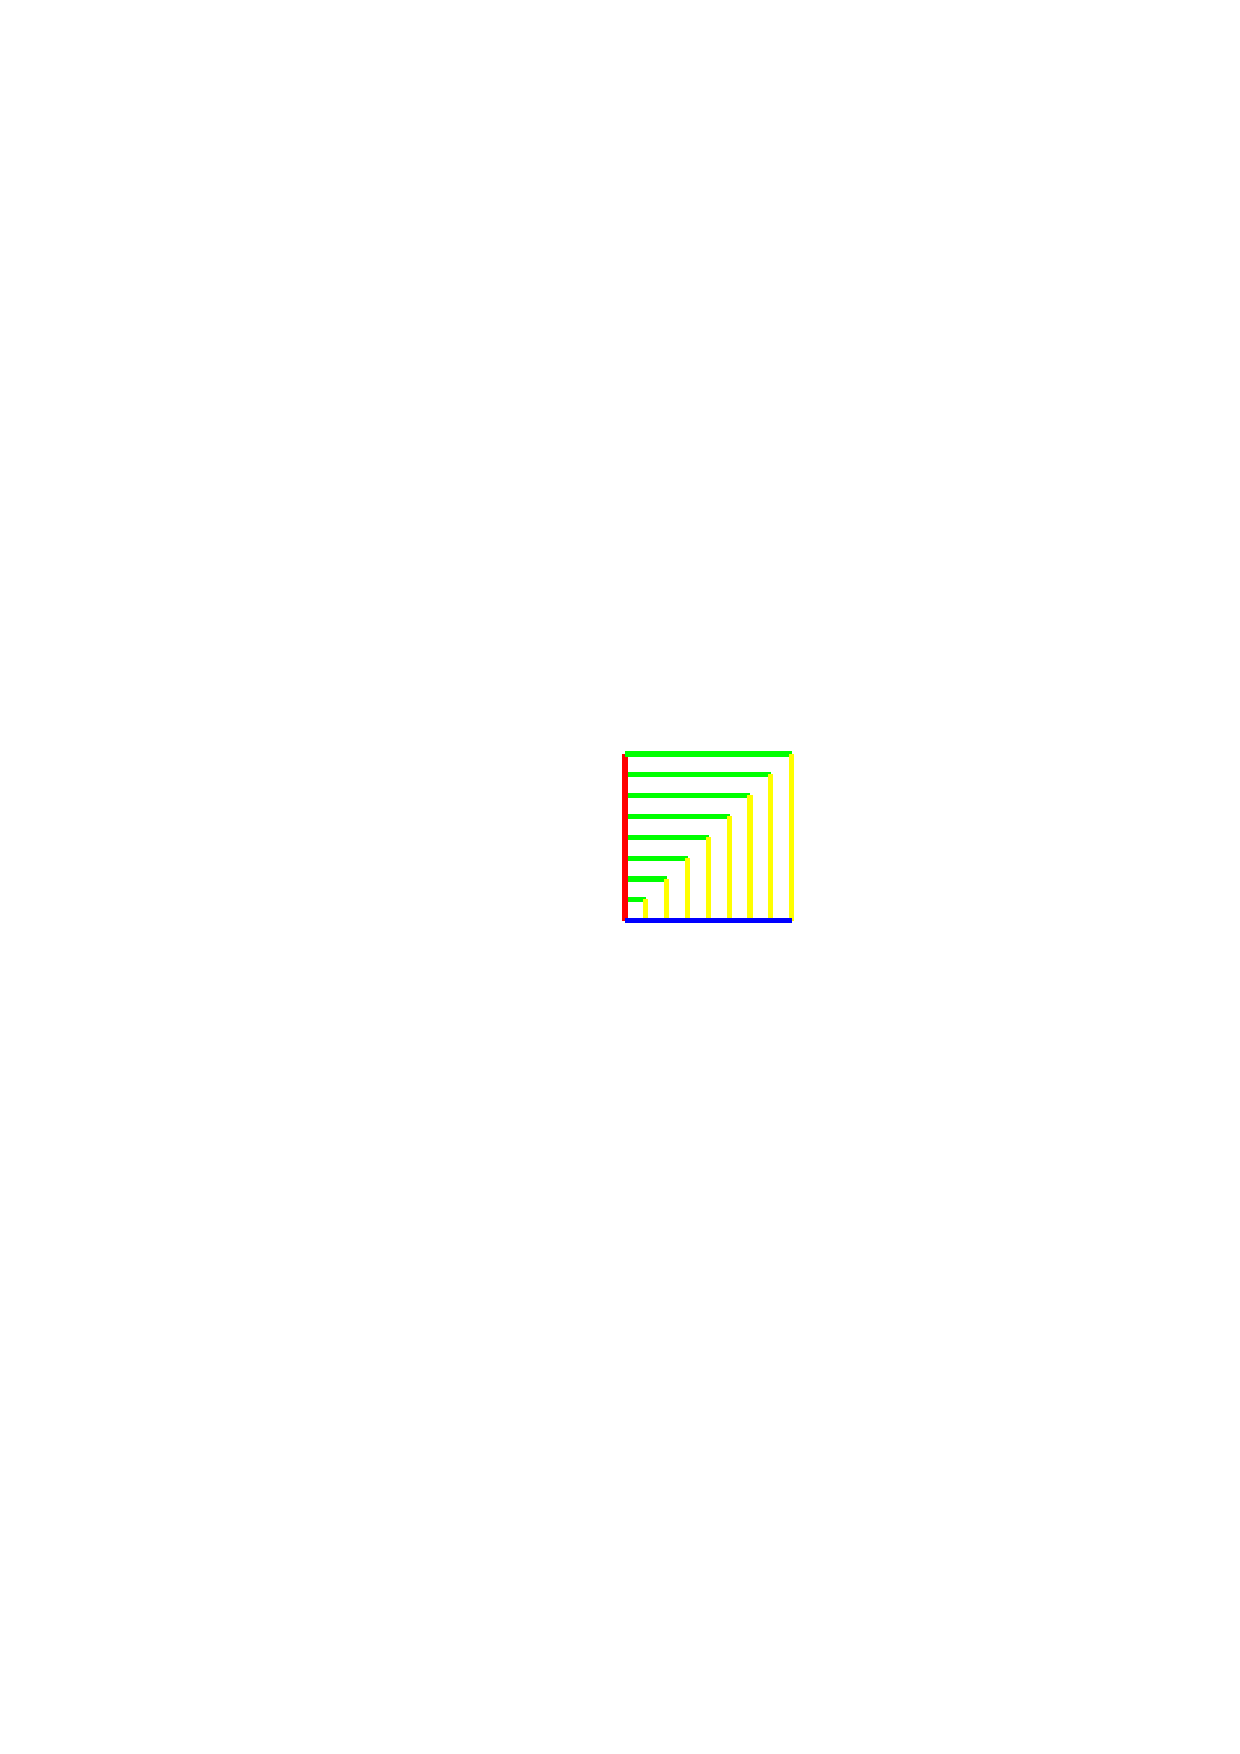
\includegraphics[clip,trim=10cm 11cm 6cm 11cm,scale=1.25]{../Pictures/out_tunnel.pdf}
\end{center}

\noindent Variables can be set using a postfix notation, e.g.~:
\begin{codesnippet}
START
   SET A ( 0 )
   SET B ( $A 1 + )
   SET C ( $B 2 * )
END
\end{codesnippet}

\subsection*{The Formal Grammar}
{\samepage
\begin{verbatim}
<PROG>   ::= "START" <INSLST>

<INSLST> ::= "END" | <INS> <INSLST>
<INS>    ::= <FWD> | <RGT> | <COL> | <LOOP> | <SET>

<FWD>    ::= "FORWARD" <VARNUM>
<RGT>    ::= "RIGHT" <VARNUM>
<COL>    ::= "COLOUR" <VAR> | "COLOUR" <WORD>
<LOOP>   ::= "LOOP" <LTR> "OVER" <LST> <INSLST>
<SET>    ::= "SET" <LTR> "(" <PFIX>

<VARNUM> ::= <VAR> | <NUM>
% Variables e.g. $A, $B, $Z etc.
<VAR>    ::= $<LTR>
% One Uppercase letter
<LTR>    ::= A, B ... Z
% Any valid double (as defined by scanf("%lf"...)
<NUM>    ::= 10 or -17.99 etc.

% A single word (as defined by scanf("%s"...) with double-quotes around it
% Valid colours include "BLACK", "RED", "GREEN", "BLUE",
% "YELLOW", "CYAN", "MAGENTA", "WHITE"
<WORD>   ::=  "RED", "BLUE", "HELLO!" or  "178"

<LST>    ::= "{" <ITEMS>
<ITEMS>  ::= "}" | <ITEM> <ITEMS>
<ITEM>   ::= <VARNUM> | <WORD>

<PFIX>   ::= ")" | <OP> <PFIX> | <VARNUM> <PFIX>
% A single mathematical operation character
<OP>     ::= + - / *
\end{verbatim}
}

\begin{exercise}

\strut\\[1em]
\vspace*{1ex}
\noindent{\bf\large Parser (35\%)}

\noindent Implement a recursive descent parser - this will report
whether or not a given turtle program follows the formal grammar or not.
The input file is specified via \verb^argv[1]^ - there is {\bf no}
output if the input file is {\bf valid}. Elsewise, a graceful non-zero
\verb^exit^ is made.  You should use the techniques described in the
lecture for this - writing code that carefully follows the grammar. For
instance, it won't use a tokenzier.

\noindent All source code will be in the \verb^Parse/^ sub-directory.

\vspace*{1em}
\noindent {\bf\large Interpreter (25\%)}

\noindent Extend the parser, so it becomes an interpreter. The
instructions are now `executed'. Do not begin a new program for this,
simply copy and then extend your existing parser. Output is to a text
file if the users specifies an \verb^argv[2]^, in the form of a 2D array
of characters where colours are represented by blac(K), (R)ed, (G)reen,
(Y)ellow, (B)lue, (M)agenta, (C)yan and (W)hite, via a $51$ wide $\times$
$33$ height array of characters e.g.:

\begin{verbatim}





                         GGGGGY
                         R    Y
                         R    Y
                         R    Y
                         R    Y
                      WWWWWWWWWWWW
                       W        W
                       W        W
                        W      W
                        W      W
                         W    W
                         W   W
                          W  W
                          W W
                           WW
                           W





\end{verbatim}

\noindent If no \verb^argv[2]^ is specified, then output is to the
screen using ANSI colour characters in same style as that used in
Section~\ref{sec:ansi}, with a $1$ second pause after each \verb^FORWARD^
instruction. 

\noindent Note that some files that successfully parse will not
successfully interpret (and vice versa) - there are example \verb^.ttl^
files provided to demonstrate this.

\noindent All interpreter source code will be in the \verb^Interp/^ sub-directory.

\vspace*{1em}
\noindent {\bf\large Postscript (5\%)}

\noindent Extend the output functionality of the
interpreter such that if \verb^argv[2]^ has a \verb^.ps^
extension, then the correct postscript instructions are written to that file.
\wwwurl{https://paulbourke.net/dataformats/postscript} Since PDFs are a
more common file format, then at the end, your program should also convert the \verb^.ps^
file to a \verb^.pdf^ file using a \verb^system()^ call in your C code
to \verb^ps2pdf^ which is installed on the lab machines. 
My implementation uses the postscript commands \verb^showpage^,
\verb^newpath^, \verb^moveto^, \verb^lineto^, \verb^setrgbcolour^, \verb^scale^
and \verb^stroke^.

If you get this to work, add it to the interpreter above - it will be tested
using both \verb^.txt^ and \verb^.ps^ output modes.

\vspace*{1ex}
\noindent {\bf\large Extension (15\%)}

\noindent Extend the project in a direction of
your choice. It should demonstrate your {\bf understanding} of some aspect
of programming or S/W engineering. If you extend the formal grammar
make sure that you give us the new, full grammar, along with the code in
the \verb^Extension/^ sub-directory named \verb^grammar.txt^, in addition to
a $300$ word (max) description of what you've achieve in \verb^extension.txt^.
Please do not submit ideas for future work, only functionality you've got working.

\vspace*{1ex}
\noindent {\bf\large Testing (20\%)}

\noindent Show the testing strategy on your code -
you should give details of any
unit testing or white/black-box testing done on your code. Describe any
test-harnesses used. Convince us that every line of your C code has
been tested, explaining the process, lessons learned and bugs found.
Submit a file \verb^testing.txt^ in the sub-directory \verb^Testing/^.

\subsection*{Hints}
\begin{itemize}

\item Understand the noughts and ones example given in the notes.

\item Don't try to write the entire program in one go. Try a cut
down version of the grammar first, e.g.:
{\small
\begin{verbatim}
<PROG>   ::= "START" <INSLST>

<INSLST> ::= "END" | <INS> <INSLST>
<INS>    ::= <FWD> | <RGT>

<FWD>    ::= "FORWARD" <NUM>
<RGT>    ::= "RIGHT" <NUM>

<NUM>    ::= 10 or -17.99 etc.
\end{verbatim}
}

\item The language is simply a sequence of words (even the braces),
so use \verb^fscanf()^.

\item Some issues, (e.g. drawing out-of-bounds), incorrect postfix
expressions cannot explained by the formal grammar. Use your own
common-sense to decide how to reconcile these, and explain what you
have done.

\item Once your parser works, extend it to become an interpreter. DO
NOT aim to parse the program first and then interpret it
separately. Interpreting and parsing are inseparably bound together. Use
our lectures notes for this and not those from other units such as
Architecture which take a very slightly different approach.

\item For the simple trigonometry required to compute the turtles
destination, bear in mind that the \verb^cos()^ and \verb^sin()^ functions
in C require parameters in radians and not degrees.

\item The turtle always begins in the centre of the screen facing due
north (upwards) and having a default white colour.  For the postscript/PDF
part, since white ink is hard to see on white paper, I've redefined
white ink to be slightly grey.

\item Start testing very early - this is a complex program to test and
trying to do it (or explain it) near the end won't work.

\end{itemize}

\subsection*{Submission}
Adapt the given Makefile if necessary to allow the parser, interpreter and extension to 
be built.
Submit your extension via text files \verb^extension.txt^ in \verb^Extension/^ along with  \verb^grammar.txt^ and your source code.

Your testing strategy will be explained in \verb^testing.txt^ along with any other files you'd like to bring our attention to in \verb^Testing/^.

Bundle this all up into a single \verb^turtle.zip file^ that contains {\bf everything} required
for us to compile and understand your code.

\end{exercise}


\begin{exercise}
Implement a recursive descent parser - this will report
whether or not a given turtle program follows the formal grammar or not.
The input file is specified via \verb^argv[1]^ - there is {\bf no} output if
the input file is {\bf valid}. Elsewise, a non-zero \verb^exit^ is made.

{\bf Extend} the parser, so it becomes an interpreter. The instructions are
now `executed'. Do not write a new program for this, simply extend your
existing parser. Output is via SDL. You may find the function call
\verb^SDL_RenderDrawLine^ useful.

Show a testing strategy on the above -
you should give details of
unit testing, white/black-box testing done on your code. Describe any
test-harnesses used. In addition, give examples of the output of many different
turtle programs. Convince me that every line of your C code
has been tested.

Show an extension to the project in a direction of
your choice. It should demonstrate your {\bf understanding} of some aspect
of programming or S/W engineering. If you extend the formal grammar
make sure that you show the new, full grammar.

\subsection*{Hints}
\begin{itemize}
\item All four sections above are equally weighted.
\item Don't try to write the entire program in one go. Try a cut
down version of the grammar first, e.g.:
{\small
\begin{verbatim}
<MAIN>        ::= "{" <INSTRCTLST>
<INSTRCTLST>  ::= <INSTRUCTION><INSTRCTLST> |
                  "}"
<INSTRUCTION> ::= <FD> | <LT> | <RT>
<FD>          ::= "FD" <VARNUM>
<LT>          ::= "LT" <VARNUM>
<RT>          ::= "RT" <VARNUM>
<VARNUM>      ::= number
\end{verbatim}
}
\item The language is simply a sequence of words (even the semi-colons),
so use \verb^fscanf()^.
\item Some issues, such as what happens if you use an undefined variable,
or if you use a variable before it is set, are not explained by the formal
grammar. Use your own common-sense, and explain what you have done.
\item Once your parser works, extend it to become an interpreter. DO NOT
aim to parse the program first and then interpret it separately. Interpreting
and parsing are inseparably bound together.
\item Start testing very early - this is a complex beast to test and trying to
do it near the end won't work.
\end{itemize}

\subsection*{Submission}
Your testing strategy will be explained in \verb^testing.txt^, and your extension
as \verb^extension.txt^. For the parser, interpreter and extension sections, make
sure there's a \verb^Makefile^, so that I can easily build the code using \verb^make parse^,
\verb^make interp^ and \verb^make extension^. Submit a single \verb^turtle.zip^ file.

\end{exercise}


\nsection{The UNIX awk program}

Sometimes handling files containing numerical data in C
may be somewhat arduous. A `simple' program to swap the first
and second columns of a file is quite long in C.

For this reason, there is a simple language called awk which
allows simple manipulation to be done on a line by line basis.
For example:
\begin{verbatim}
{
print $2, $1;
}
\end{verbatim}
swaps the first and second fields in a file.
The whole program is applied to every line of the input file in turn.

Other examples of awk would include printing fields in reverse order:
\begin{verbatim}
{ for (i = NF; i > 0; --i) print $i }
\end{verbatim}

\noindent Adding up first column, print sum and average
\begin{verbatim}
{ s += $1 }
END{print "sum is",s," average is",s/NR}
\end{verbatim}

\noindent Notice the `special' variables \verb^NR^ and \verb^NF^.
Other special variables include \verb^FS^ which defines how
fields are separated (default space and tab).
See `man awk' for more information.

\subsection*{The CAWK formal grammar}

This assignment involves writing a recursive descent parser
for a simple, cut-down version of awk called `cawk'. It is based
on the following formal grammar:

{\small
\begin{verbatim}
<PROG>       := "{" <ILST> |
                "{" <ILST> "END" "{" <ILST>
<ILST>       := <INSTR> <ILST> | "}"
<INSTR>      := <LET> | <IF> | <PRINT> | <FOR>
<LET>        := "LET" <USER> "=" <POLISH> 
<USER>       : = "$A" | .. | "$Z"
<RD>         := <USER> | "$[" <INDEX> "]" | <SPEC>
<INDEX>      := number | <USER> | <SPEC>
<SPEC>       := "$#" | "$@"
<NUMVAR>     := number | <RD>
<POLISH>     := <OPER><POLISH> | ";"
<OPER>       := <NUMVAR> | <OPERATOR>
<OPERATOR>   := "+" | "-" | "*" | "/"
<IF>         := "IF" "(" <TEST> ")" "{" <ILST>
<TEST>       := <NUMVAR> <COND> <NUMVAR>
<COND>       := "<" | ">" | "==" | "!="
<PRINT>      := "PRINT" <NUMVAR> | "PRINT" string
<FOR>        := "FOR" <USER> "=" <NUMVAR> "TO"
                <NUMVAR> "STEP" <NUMVAR> "{" <ILST>
\end{verbatim}

\noindent Note, you may assume that the program consists of
a list of words separated by white-space.
\begin{verbatim}
$# is the number of records.
$@ is the number of fields in the current record.
$[ 0 ] is the entire line
$[ i ] is the ith field of the record 
\end{verbatim}
}

\section*{Examples of CAWK}
\begin{verbatim}
{
PRINT $[ 2 ]
PRINT $[ 1 ]
PRINT "\n"
}
\end{verbatim}

\noindent Print fields in reverse order:
\begin{verbatim}
{
   FOR $I = $@ TO 1 STEP -1 {
      PRINT $[ $I ]
   }
   PRINT "\n"
}
\end{verbatim}


\begin{exercise}
Write a C program to implement the above formal grammar. Your program
should read in a cawk program (argv[1]) and expect the data
file to be read from standard input (or from argv[2] if specified).

The marks are split as follows:
\begin{itemize}
\item (25\%) To implement a recursive descent parser - this says
whether or not a given CAWK program follows the formal grammar or not.

\item (25\%) To implement an interpreter, so that the instructions are
executed.

\item (25\%) To show a testing strategy on the above -
you should give details of
white-box and black-box testing done on your code. Describe any
test-harnesses used. Give examples of the output of many different
cawk programs.

\item (25\%) To show an extension to the project in a direction of
your choice. It should demonstrate your understanding of some aspect
of programming or S/W engineering. If you extend the formal grammar
make sure that you show the new, full grammar.
\end{itemize}

Submit the program(s) and a Makefile so that I can:

\begin{itemize}
\item Compile the parser by typing `make parse'.
\item Compile the interpreter by typing `make interp'.
\item Compile the extension by typing `make extension'.
\end{itemize}

In addition:
\begin{itemize}
\item Submit a test strategy report called test.txt. This will include
sample outputs, any code written especially for testing etc.
\item Submit an extension report called `extend.txt'. This is quite
brief and explains the extension attempted.
\end{itemize}

\end{exercise}

\nsection{Neill's Adventure Language}

Some of the very earliest computer games were text-based adventures e.g.
Colossal Cave \wwwurl{https://en.wikipedia.org/wiki/Colossal_Cave_Adventure}

Here we write a simple language (NAL) which allows us to write (simplified) versions of such games, focussing on setting variables and printing.
The grammar is as follows:
\begin{codesnippet}
<PROGRAM>   := "{" <INSTRS>
<INSTRS>    := "}" | <INSTRUCT> <INSTRS>
<INSTRUCT>  := <FILE> | <ABORT> | <INPUT> | <IFCOND> | <INC> | <SET> |
               <JUMP> | <PRINT> | <RND>

% Execute the instructions in file, then return here e.g. :
% FILE "test1.nal"
<FILE>      := "FILE" <STRCON>

% Halt/abort all execution right now !
<ABORT>     := "ABORT"

% Fill a number-variable with a number, or 2 string-variables with string :
% IN2STR ( $C, $ZER )  or  INNUM ( %NV ) 
<INPUT>     := "IN2STR" "(" <STRVAR> "," <STRVAR> ")" | "INNUM" "(" <NUMVAR> ")"

% Jump to the nth word in this file (the first word is number zero!)
% Brackets count as one word, "things in quotes" count as one word, e.g. :
% JUMP 5
<JUMP>      := "JUMP" <NUMCON> 

% Output the value of variable, or constant, to screen with (without a linefeed)
<PRINT>     := "PRINT" <VARCON>
<PRINTN>    := "PRINTN" <VARCON>

% Set a variable to a random number in the range 0 - 99 e.g. :
% RND ( %N )
% Number should be seeded via the clock to be different on successive executions
<RND>      := "RND" "(" <NUMVAR> ")"

% If condition/test is true, execute INSTRS after brace, else skip braces
<IFCOND>    := <IFEQUAL> "{" <INSTRS> | <IFGREATER> "{" <INSTRS>
<IFEQUAL>   := "IFEQUAL" "(" <VARCON> "," <VARCON> ")"
<IFGREATER> := "IFGREATER" "(" <VARCON> "," <VARCON> ")"

% Add 1 to a number-variable e.g. :
% INC ( %ABC )
<INC>       := "INC" "(" <NUMVAR> ")"

% Set a variable. All variables are GLOBAL, and persist across the use of FILE etc.
% $A = "Hello"  or  %B = 17.6
<SET>       := <VAR> "=" <VARCON>

% Some helpful variable/constant rules
% (Here ROT18 is ROT13 for letters and rot5 for digits)
<VARCON>    := <VAR> | <CON>
<VAR>       := <STRVAR> | <NUMVAR>
<CON>       := <STRCON> | <NUMCON>
<STRVAR>    := $[A-Z]+
<NUMVAR>    := %[A-Z]+
<STRCON>    := A plain-text string in double-quotes, e.g. "HELLO.TXT",
               or a ROT18 string in hashes e.g. #URYYB.GKG#
<NUMCON>    := A number e.g. 14.301
\end{codesnippet}

Note that string constants can be entered via the use of double quotes, or using hashes to encode strings using ROT18 \wwwurl{https://en.wikipedia.org/wiki/ROT13}
in which characters are encoded/decoded according to:
\begin{terminaloutput}
Plain: ABCDEFGHIJKLMNOPQRSTUVWXYZ
ROT13: NOPQRSTUVWXYZABCDEFGHIJKLM
Plain: abcdefghijklmnopqrstuvwxyz
ROT13: nopqrstuvwxyzabcdefghijklm
Plain: 0123456789
ROT5 : 5678901234
\end{terminaloutput}
the algorithm allows obvious `spoilers' to be hidden from users
browsing through \verb^.nal^ files, but is simple to apply.

A simple program showing the use of assignment, conditionals and ROT18 is shown:
\begin{codesnippet}
{
   $A = "Neill"
   %E = 12.4
   IFEQUAL ( $A , #Arvyy# ) {
      PRINT #Uryyb Jbeyq!#
   }
}
\end{codesnippet}
Here string-variables \verb^($)^ and number-variables \verb^(%)^ are
initialised.

The use of `JUMP' is shown next - this allows execution to move a chosen word in the program. Strings inside quotes count as one word, so the following contains six words:
\begin{codesnippet}
{
   PRINT "Warning : Infinite Loop !"
   JUMP 1
}
\end{codesnippet}
`FILE' allows another file to be executed (as <PROG>) and then execution returns to the original when finished. All variables are shared across files and are global:
\begin{codesnippet}
{
   PRINT "In test4, before"
   FILE "test1.nal"
   PRINT "In test4, after"
}
\end{codesnippet}
`RND' sets a variable to a number in the range $0 - 99$, while `INC' adds one to a number-variable.
\begin{codesnippet}
{
   %C = 0
   RND ( %A )
   PRINT %A
   INC ( %C )
   IFGREATER ( %C , 9 ) {
      ABORT
   }
   JUMP 4
}
\end{codesnippet}
`ABORT' halts execution instantly.

A simple guessing game is shown below:
\begin{codesnippet}
{

   PRINT "I'm thinking of a number (0-99).\nCan you guess it?"
   RND ( %MINE )
   %CNT = 0

   INC ( %CNT )
   PRINT "Type in your guess"
   INNUM ( %GUESS )
   IFGREATER ( %CNT , 7 ) {
      PRINT #Gbb znal gevrf :-(#
      ABORT
   }
   IFGREATER ( %GUESS , %MINE ) {
      PRINT "Too Big ! Try again ... "
      JUMP 10
   }
   IFGREATER ( %MINE , %GUESS ) {
      PRINT "Too Small ! Try again ... "
      JUMP 10
   }
   IFEQUAL ( %MINE , %GUESS ) {
      PRINT #Lbh thrffrq pbeerpgyl, lbh jva :-)#
      PRINTN "Number of goes = "
      PRINT %CNT
      ABORT
   }

}
\end{codesnippet}
`INNUM' gets a number (float) from the user, and the use of `PRINT' (with a newline after), and `PRINTN' (without a newline after) is demonstrated.

\begin{exercise}
\begin{itemize}

\strut

\item {\bf (40\%)}
Implement a parser. The \verb^.nal^ file should be read in using
\verb^argv[1]^.  If the file is parsed correctly, the only output should
be:
\begin{terminaloutput}
Parsed OK
\end{terminaloutput}

\item {\bf (30\%)}
Implement an interpreter, building on top of the parser in the
manner described in the lectures. Do not write a brand new program -
interpretation will be done alongside parsing.

\item {\bf (20\%)}
Submit the testing you have undertaken, including examples and a
description of your strategies. This should convince us that you have
tested every line of code, and that it works correctly. If there are
still issues/bugs state them clearly. Also, point out any bugs that
you have successfully found using these approaches. Submit a file named
\verb^testing.txt^, along with any other files you feel necessary. Due
to the recursive nature of this assignment testing is non-trivial -
simply submitting many \verb^.nal^ files that `work' is not sufficient.
No particular strategy is mandated. You may wish to explore a couple
and briefly discuss strengths and weaknesses.

\item {\bf (10\%)}
Undertake an extension of your choosing.  Remember, that the assessment is
based on the quality of your coding, so choose something to demonstrate
an aspect of programming or software engineering that you haven't
had a chance to use in the main assignment. Submit a file named
\verb^extension.txt^ outlining, in brief, your contribution.
\end{itemize}

\subsection*{Hints}
\begin{itemize}
\item Don't try to write the entire program in one go. Try a cut
down version of the grammar first. Build-up from the \verb^01s^
example given in lectures.
\item Some issues, such as what happens if you use an undefined variable,
or if you use a variable before it is set, are not explained by the formal
grammar. Use your own common-sense, and explain what you have done.
\item Once your parser works, extend it to become an interpreter. DO NOT
aim to parse the program first and then interpret it separately.
Interpreting and parsing are inseparably bound together.
\end{itemize}
 
\subsection*{Submission}

Your testing strategy will be explained in \verb^testing.txt^, and
your extension as \verb^extension.txt^. For the parser, interpreter
and extension sections , make sure there's one \verb^Makefile^, so that I
can easily build the code using \verb^make parse^, \verb^make interp^
and \verb^make extension^. I've given an example \verb^makefile^ in the
usual place, but this is an example only - yours may be different.
I wrote only one program \verb^nal.c^ and built the two
different version by setting a \verb^#define^ {\bf via the makefile with}
\verb^-DINTERP^. Inside the code itself \verb^#ifdef INTERP^ and \verb^#endif^ are used.
Also make sure that basic testing is available using \verb^make testparse^ and \verb^make testinterp^.

\noindent Place all the files required for your submission in a single \verb^.zip^ file called \verb^nal.zip^ - this file will not contain other zipped files.

\end{exercise}


\appendix
\begin{appendices}

\chapterimage{../Pictures/style.jpg}
\chapter{House Style}
\nsection{Correctness}

These style rules ensure your code is as-correct-as-can-be with the aid
of the compiler and other tools:
\begin{description}
\item[FLAGS] Having no warnings (or errors!) when compiling and executing with the flags:\\
For array bounds checking, \verb^NULL^ pointers being dereferenced etc:
\begin{terminaloutput}
-Wall -Wextra -Wfloat-equal -Wvla -pedantic -std=c99
-fsanitize=undefined -fsanitize=address -g3
\end{terminaloutput}
For memory leaks:
\begin{terminaloutput}
-Wall -Wextra -Wfloat-equal -Wvla -pedantic -std=c99
-g3
\end{terminaloutput}
then run:
\begin{terminaloutput}
valgrind --leak-check=full ./myexec
\end{terminaloutput}
For `final' production-ready code:
\begin{terminaloutput}
-Wall -Wextra -Wfloat-equal -Wvla -pedantic -std=c99
-O3
\end{terminaloutput}

You can use more flags than this, obviously, but these will
make sure a few of the essential warnings that commonly indicate
the presence of bugs and leaks are checked. These guidelines are meant to
be independent of the particular compiler used though. Sometimes it is helpful to use many compilers too, e.g. \verb^gcc^ and \verb^clang^.

If you have unused variables (for example) in your code, it doesn't matter whether your compiler happened to tell you about it or not - it's still wrong !

\item[BRACE] Always brace all functions, \verb^for^s, \verb^while^s, \verb^if/else^ etc.
Somewhat contraversial, this ensures that `extra' lines tagged onto loops are
dealt with correctly. For instance:
\begin{codesnippet}
while(i < 10)
   printf("%i\n", i);
   i++;
\end{codesnippet}
looks like it should print out \verb^i^ $10$ times, but instead runs infinitely.
The programmer probably meant:
\begin{codesnippet}
while(i < 10){
   printf("%i\n", i);
   i++;
}
\end{codesnippet}

\item[GOTO] You do not use any of the keywords \verb^continue^, \verb^goto^ or \verb^break^. The one exception is inside \verb^switch^, where \verb^break^ is allowed because it is essential !
These keywords usually lead to tangled and complex `spaghetti' coding style.
I often recommend that you rewrite the offending code uing functions, which {\bf can} have multiple \verb^return^s
in them.

\item[NAMES] Meaningful identifiers. Make sure that functions names and variables having meaningful, but succinct,  names.

\item[REPC] Repetitive code. If you've cut-and-paste large chunks of code, and made minor changes to it, you've done it wrong. Make it a function, and pass parameters that make the changes required.
\begin{codesnippet}
int inbounds1(int i){
   if(i >=0 && i < MAX){
      return 1;
   }
   else{ 
      return 0;
   }
}

int inbounds2(int i){
   if(i >=0 && i < LEN){
      return 1;
   }
   else{ 
      return 0;
   }
}
\end{codesnippet}
might make more sense as:
\begin{codesnippet}
int inbounds2(int i, int mx){
   if(i >=0 && i < mx){
      return 1;
   }
   else{ 
      return 0;
   }
}
\end{codesnippet}

\item[GLOB] No global variables. Global variables are declared `above' \verb^main()^, are in scope of all functions, and can be altered {\bf anywhere} in the code. This makes it rather unclear {\bf which} functions should be reading or writing them. You can make a case for saying that occasionally they could be useful (or better) than the alternatives, but for now, they are banned !

\item[RETV] Any functions that returns a value, should have it used:
\begin{codesnippet}
scanf("%i", &i);
\end{codesnippet}
is incorrect. It returns a value that is ignored. Instead do:
\begin{codesnippet}
	if(scanf("%i", &i) != 1{
	   /* PANIC */
\end{codesnippet}

The only exceptions are \verb^printf^ and \verb^putchar^ which do return values but
which are typically ignored.

\item[MATCH] For every \verb^fopen^ there should be a matching \verb^fclose^.
For every \verb^malloc^ there should be a \verb^free^.
This helps avoid memory leaks, when your program or functions are later used
in a larger project.

\item[STDERR] When exiting your program in an error state, make sure that you \verb^fprintf^ the error on \verb^stderr^ and not \verb^stdout^. Use \verb^exit^, e.g.
\begin{codesnippet}
if(argc != 2){
   fprintf(stderr, "Usage : %s <filename>\n", argv[0]);
   exit(EXIT_FAILURE);
}
\end{codesnippet}


\end{description}

\nsection{Prettifying}

These rules are about making your code easier to read and having a consistent
style in a form that others are expecting to see.

\begin{description}

\item[LLEN] Line length. Many people use terminal and editors that are
of a fixed-width. Having excessively long lines may cause the viewer to scroll to
off the screen. Keep lines short, perhaps $< 60$ characters. However, in a similar way
to the {\bf FLEN} rule below, it's really about the complexity of the line that's the issue,
not its absolute length. A programmer would generally find:
{\small
\begin{codesnippet}
bool arrcleanse(cell oldarr[HEIGHT][WIDTH], cell newarr[HEIGHT][WIDTH], int h, int w)
\end{codesnippet}
}
a great deal easier to read than:
\begin{codesnippet}
if(a < b && j++ >= szpar(e ? true : false) || h==4){
\end{codesnippet}
despite it being twice as long.

\item[TABS] Don't use tabs to indent your code. Every editor views these differently, so you have no guarentee that I'm seeing the same layout as you do. Use spaces. This also prevents issues when cuttig-and-pasting from one source to another.

\item[INDENT] Indentation: choose a style for indentation
and keep to it. I happen to use $3$ spaces, put opening braces
for functions on a new line, but at the end of \verb^if^,\verb^else^, \verb^for^, \verb^while^ etc, then close them on a new line, underneath the `i' of the \verb^if^:
\begin{codesnippet}
int smallest(int a, int b)
{
   if(a < b){
      return a;
   }
   else{
      return b;
   }
}
\end{codesnippet}
You can use any style you like, as long as it's consistent.

\item[MAIN] The code should have function prototypes/definitions first, then \verb^main()^, followed by the function implementation. This means the reader always know where to find \verb^main()^, since it will be near the top of the file.


\item[CAPS] Constants are \verb^#define^d, and use all CAPITALS. For instance:
\begin{codesnippet}
#define WEEKS 52
#define MAX(a,b) (a < b ? b:a)
\end{codesnippet}


\item[FLEN] Short functions. All functions are short. It's quite
difficult to put a maximum number of lines on this, but use $20$ as a
starting point. Exceptions include a function that simply prints a list
of instructions. There would be no benefit in splitting it into smaller
functions. Short functions are easier to plan, write and test.

I find it more useful to think about how hard the function is to
understand, rather than its length. Therefore, a $30$ line, simple
function is fine, but an extremely complex and dense $15$ line function
might need to be split up, or more self-documentation added.


\end{description}

\nsection{Readability}

Your code should be self-documenting. Comments will be written when there
is something complex to explain, and only read when something has gone
catastrophically wrong. In many cases clever use of coding will avoid the
need for them.  The compiler never sees them, so cannot check them. If you
change your code, but not your comments, they can be highly misleading.

As Kevlin Henney said~:
\begin{quote}
A common fallacy is to assume authors of incomprehensible code will somehow
be able to express themselves lucidly and clearly in comments. 
\end{quote}

\begin{description}
\item[MAGIC] No magic numbers. There should be no inexplicable numbers in your code, such
as:
\begin{codesnippet}
	if(i < 36){
\end{codesnippet}

It's probably unclear to the reader where the $36$ has come from, or what it means,
even if it is obvious to the programmer at the time of writing the code. Instead,
\verb^#define^ them with a meaningful name.
Array overruns are often cured by being consistent with \verb^#define^s.

\item[BRIEF] Comments are brief, and non-trivial. Worthless commenting often
looks something like:
\begin{codesnippet}
// Set the variable i to zero
int i = 0;
\end{codesnippet}
The programmer extracts no additional information from it. However, for more
difficult edge cases, a comment might be useful.
\begin{codesnippet}
// Have we reached the end of the list ?
if(t1->h == NULL){ 
\end{codesnippet}

\noindent To prevent lines from becoming too long, it is good practice to put comments above
the line it refers to, not at the end of the same line.

\item[TYPE] You should use \verb^typedef^s, \verb^enum^s and \verb^struct^s to
increase readability. 

\item[INFIN] No loops should be infinite. I'll never ask you to write a program that is meant to run forever. Therefore statements such as
\begin{codesnippet}
while(1){
\end{codesnippet}
or
\begin{codesnippet}
for(;;;){
\end{codesnippet}
are to be avoided.

\item[2DINDEX] 2D Arrays in C are indexed \verb^[row][col]^.  Sometimes
it may still work correctly, especially if you've consistently confused
the two.  Therefore, if you write code that indexes it \verb^[col][row]^,
or \verb^[x][y]^ it will confuse anyone else trying to understand (or
reuse) your code. If you were to sketch a graph using \verb^(i,j)^ you'd
almost certainly make $i$ the horizontal axis, and $j$ the vertical.
Therfore, for any two variables it makes more sense to write \verb^[b][a]^
or \verb^[j][i]^.

\end{description}



\chapterimage{../Pictures/exam.jpg}
\chapter{Lab Tests}

\section*{Examination Rules}
This is an exam. Please:
\begin{itemize}
\item Wait to be seated by a Lab.\ supervisor.
\item Do not talk to anyone else.
\item Do not use a Web browser, unless instructed to do so (e.g. to submit files).
\item Do not use an email connection.
\item Do not use other electronic devices such as laptops, tablets or phones.
\item Do not look in other peoples directories.
\item Do not use code written in `groups' with others students.
\item {\bf DO} use text books, lecture notes, man pages etc.
\end{itemize}
If you do not obey the above rules you will be asked to leave.

People arriving late may not be allowed into the Lab.

You have one hour. There is additional time in case a
server crashes or some other problem occurs.

\section*{Submitting Your Work}
As you complete each part, submit it online using the Blackboard
submission system. Do not submit files that don't work.

For multi-part questions, if you complete Part~1, submit a file called \verb^part1.c^.\\
If you complete Part~2, submit a file called \verb^part2.c^ and so on.

No partial marks are available.
The only possible scores for each sub-part are pass (100\%) or fail (0\%).

\section*{Code Style}
\begin{itemize}
\item Your code {bf must} compile without warnings using the gcc flags:
\begin{verbatim}
-pedantic -Wall -Wextra -Wfloat-equal -ansi -O2
\end{verbatim}
\item Do {\bf NOT} use any global variables.
%\item {\bf If} you need to use \verb^rand()^ in your code, feel free to set
%the seed of the random number generator to give different outputs
%each time your program is run, for instance using~:
%\begin{verbatim}
%srand(time(NULL));
%\end{verbatim}
%remembering to \verb^#include <time.h>^
\end{itemize}


\newpage
\nsection{Anagrams}
\subsection*{Part 1 (60\%)}

An anagram is a rearrangement of a word, using all the letters.
Two words are said to be anagrams if they have the same characters,
but in a different order.
For instance the words `parsley', `players' and `replays'
are all anagrams of each other.

Since you need to rearrange the words, two identical words, by definition, are not anagrams.

Using the following template, fill in the function \verb^anagram()^,
so that the program runs successfully~:
\begin{verbatim}
#include <stdio.h>
#include <string.h>
#include <ctype.h>
#include <assert.h>

int anagram(char s1[], char s2[]);

int main(void)
{
   assert(anagram("elvis", "lives") == 1);
   assert(anagram("dreads", "sadder") == 1);
   assert(anagram("replays", "parsley") == 1);
   assert(anagram("listen", "silent") == 1);
   assert(anagram("orchestra", "carthorse") == 1);

   /* Two identical words are not anagrams */
   assert(anagram("elvis", "elvis") == 0);

   assert(anagram("neill", "neil") == 0);
   assert(anagram("neil", "neill") == 0);
   assert(anagram("horse", "short") == 0);

   return 0;
}

int anagram(char s1[], char s2[])
{


}
\end{verbatim} 

Obviously, your program will need to run for other, unseen but similar, test cases. 

\subsection*{Part 2 (40\%)}

A deranged anagram has two words with the same characters, but the same
character does not appear in the same position.

The words `elvis' and `lives' are not a derangement since the `s' is
in the same position in both words.
However, `dreads' and `sadder' are, since no letter appears in the
same position between the two words.

Extend the program above so that the following assertions, inside \verb^main()^
are correct:
\begin{verbatim}
   assert(derange("elvis", "lives") == 0);
   assert(derange("dreads", "sadder") == 1);
   assert(derange("replays", "parsley") == 1);
   assert(derange("listen", "silent") == 0);
   assert(derange("orchestra", "carthorse") == 1);
\end{verbatim}



\nsection{Isograms}
\subsection*{Part 1 (60\%)}

An isogram is a word that has no repeating letters. For instance the words `graciously', `disgraceful' and
`productively' are all isograms. However, the word `dazzlingly' is not (it contains the letters `z' and `l'
twice).

Using the following template, fill in the function \verb^isogram()^, so that the program runs
successfully~:
\begin{verbatim}
#include <stdio.h>
#include <string.h>
#include <ctype.h>
#include <assert.h>

int isogram(char *s);

int main(void)
{
   assert(isogram("programming") == 0);
   assert(isogram("housewarmings") == 0);
   assert(isogram("abductions") == 1);
   assert(isogram("housewarming") == 1);
   assert(isogram("hydromagnetics") == 1);
   assert(isogram("uncopyrightable") == 1);
   return 0;
}

int isogram(char *s)
{


}
\end{verbatim} 

\subsection*{Part 2 (40\%)}
Using the \verb^isogram()^ function written above, write a program which finds the {\it longest} isogram in a
file of words. The name of the file is provided via the use of \verb^argv^.
On success, the program simply outputs the longest word and its length, nothing else. For
example~:
\begin{verbatim}
$ ./parttwo eowl_shuffle.txt
waveringly (10)
\end{verbatim}

The file may contain many isograms of (equal) longest length. In this case,
outputting any one of them will do. 

\nsection{Mutating Boards}
\subsection*{Part 1 (60\%)}

Write a {\bf function} that fills up a square board, randomly,
with an integer $0 \dots 9$. Use a:\\
\verb^#define N 20^\\
to define the size of the board.  Write another function to print the board.
The board may look something like:

{\small
\begin{verbatim}
36753562912709360626
18792023759228973612
93194784503610632061
55476569374525474430
78688431492068926649
50487172722610615949
09177115977673656394
81293908850963856115
98481030444476317596
21785741859753883189
64333860488897764303
09254059469224775481
28936802105110850646
25862847240629908131
10340391969338056640
04626756987282996027
61321599149107587048
04296104222055290283
80409196254499360502
94351743146942264128
\end{verbatim}
}

Write a
function to `mutate' the board. Mutating is done like this:
\begin{itemize}
\item Choose two random locations which are {\bf horizontally adjacent} (next to each other left-right).
\item Swap these two numbers on the board if the left one is greater than the right one, numerically.
\item Choose two random locations which are {\bf vertically adjacent} (next to each other up-down).
\item Swap these two numbers on the board if the upper one is greater than the lower one, numerically.
\item Repeat the above steps (N*N*N) times.
\end{itemize}

Now print out the board. It should look something like :
{\small
\begin{verbatim}
00000000000001111224
00000001111111233456
00000111112222244456
00001122222333445666
00112222223333555667
01112223333334556678
01112223334445556779
01122333344445556789
01223334444455666789
01223344445556666789
01223344455666667789
01224444456666777889
01234455566677777889
01234555666677788899
01234555666778888899
12234566677788888999
12345567777888889999
12445677788888899999
34446678889999999999
46678899999999999999
\end{verbatim}
}

Ensure that if you change the size of your array, by changing your \verb^#define^
that the program still operates correctly.

\subsection*{Part 2 (40\%)}
Adapt the code above, so that the algorithm is:
\begin{itemize}
\item Choose two numbers at random locations on the board.
\item Check that of these two numbers, the one closest to the centre of the array
is numerically less than the number furthest away from the centre. If not, swap them.
\item Repeat the above steps (N*N*N*N) times.
\end{itemize}

Once again randomise the array initially, and ensure that after changing your \verb^#define^
the program still works correctly.

When $N=21$, the array may look something like:
{\samepage
{\small
\begin{verbatim}
999998887777788899999
999987666656666788999
998876554444555678899
998665443333444566889
987654333222233456789
876543322112223345678
865443211111112334568
765432111000011234568
765422100000001234567
764321100000001223467
764321100000001123457
764322100000001223467
765422100000001224567
865432110000011234568
865432211111122334568
876543322212223345678
987654333222233456789
988665444333344567889
998876555444455678899
999887666656666789999
999998887777788899999
\end{verbatim}
}
}

\end{appendices}
\end{document}
